% This file was created (at least in part) by the script ParseMdtoLatex by Louis du Plessis
% (Available from https://github.com/taming-the-beast)

\documentclass[11pt]{article}
%%%%%%%%%%%%%%%%%%%%%%%%%%%%%%%%%%%%%%%%%%%%%%%%%%%%%%%%%%%%%%%
% DO NOT EDIT THIS FILE UNLESS YOU KNOW WHAT YOU ARE DOING!!! %
%%%%%%%%%%%%%%%%%%%%%%%%%%%%%%%%%%%%%%%%%%%%%%%%%%%%%%%%%%%%%%%

% Useful packages
\usepackage[]{authblk}
\usepackage{graphicx}
\usepackage{color}
\usepackage{longtable}
\usepackage{hanging}
\usepackage{indentfirst}
\usepackage{setspace}
\usepackage{enumitem}
\usepackage{verbatim}
\usepackage{upgreek}
\usepackage{framed}
\usepackage{textcomp}
\usepackage{url}
\usepackage{soul}
\usepackage{amsmath,amsfonts,amssymb,mathrsfs}
\usepackage{fancyhdr}
\usepackage[compact]{titlesec}
\usepackage[T1]{fontenc}
\usepackage{lmodern}
\usepackage[utf8]{inputenc}
\usepackage[]{listings}
%\usepackage{fontspec}
\usepackage{placeins}
\usepackage{epstopdf}
\usepackage[export]{adjustbox}
\usepackage{tikz}
\usepackage[breaklinks]{hyperref}
\usepackage[all]{hypcap}


% References
\usepackage[backend=bibtex,hyperref=true,citestyle=authoryear,bibstyle=authortitle,firstinits=true,terseinits=true,doi=false,url=false,eprint=false,maxbibnames=10,maxcitenames=2]{biblatex}
\DeclareCiteCommand{\cite}
  {\usebibmacro{prenote}}
  {\usebibmacro{citeindex}%
   \printtext[bibhyperref]{\usebibmacro{cite}}}
  {\multicitedelim}
  {\usebibmacro{postnote}}

\DeclareCiteCommand*{\cite}
  {\usebibmacro{prenote}}
  {\usebibmacro{citeindex}%
   \printtext[bibhyperref]{\usebibmacro{citeyear}}}
  {\multicitedelim}
  {\usebibmacro{postnote}}

\DeclareCiteCommand{\parencite}[\mkbibparens]
  {\usebibmacro{prenote}}
  {\usebibmacro{citeindex}%
    \printtext[bibhyperref]{\usebibmacro{cite}}}
  {\multicitedelim}
  {\usebibmacro{postnote}}

\DeclareCiteCommand*{\parencite}[\mkbibparens]
  {\usebibmacro{prenote}}
  {\usebibmacro{citeindex}%
    \printtext[bibhyperref]{\usebibmacro{citeyear}}}
  {\multicitedelim}
  {\usebibmacro{postnote}}

\DeclareCiteCommand{\footcite}[\mkbibfootnote]
  {\usebibmacro{prenote}}
  {\usebibmacro{citeindex}%
  \printtext[bibhyperref]{ \usebibmacro{cite}}}
  {\multicitedelim}
  {\usebibmacro{postnote}}

\DeclareCiteCommand{\footcitetext}[\mkbibfootnotetext]
  {\usebibmacro{prenote}}
  {\usebibmacro{citeindex}%
   \printtext[bibhyperref]{\usebibmacro{cite}}}
  {\multicitedelim}
  {\usebibmacro{postnote}}

\DeclareCiteCommand{\textcite}
  {\boolfalse{cbx:parens}}
  {\usebibmacro{citeindex}%
   \printtext[bibhyperref]{\usebibmacro{textcite}}}
  {\ifbool{cbx:parens}
     {\bibcloseparen\global\boolfalse{cbx:parens}}
     {}%
   \multicitedelim}
  {\usebibmacro{textcite:postnote}}

\newcommand{\citep}{\parencite}
\newcommand{\citet}{\textcite}
\defbibheading{relevref}[\refname]{\section*{Relevant References}}

\renewcommand{\postnotedelim}{\iffieldpages{postnote}{\addcolon}{\addcomma\space}} 
\DeclareFieldFormat{postnote}{#1} 

\DeclareFieldFormat[article, inbook, incollection, inproceedings, patent, thesis, unpublished]{title}{#1}
\DeclareFieldFormat[article, inbook, incollection, inproceedings, patent, thesis, unpublished]{journaltitle}{\mkbibemph{#1}\nopunct}
\DeclareFieldFormat[article, inbook, incollection, inproceedings, patent, thesis, unpublished]{volume}{{#1}\addcolon} %puts volume number in parens
%\DeclareFieldFormat[article, inbook, incollection, inproceedings, patent, thesis, unpublished]{year}{\mkbibparens{#1}\nopunct} %puts year in parens

\DeclareFieldFormat[article, incollection, patent, thesis, unpublished]{pages}{{\nopp#1}}

\DeclareFieldFormat{sentencecase}{\MakeSentenceCase{#1}}

\renewbibmacro*{title}{%
  \ifthenelse{\iffieldundef{title}\AND\iffieldundef{subtitle}}
    {}
    {\ifthenelse{\ifentrytype{article}\OR\ifentrytype{inbook}%
      \OR\ifentrytype{incollection}\OR\ifentrytype{inproceedings}%
      \OR\ifentrytype{inreference}}
      {\printtext[title]{%
        \printfield[sentencecase]{title}%
        \setunit{\subtitlepunct}%
        \printfield[sentencecase]{subtitle}}}%
      {\printtext[title]{%
        \printfield[titlecase]{title}%
        \setunit{\subtitlepunct}%
        \printfield[titlecase]{subtitle}}}%
     \newunit}%
  \printfield{titleaddon}}

\DefineBibliographyStrings{english}{% various adjustments to common bib entry strings
urlseen = {Accessed:},% What goes in front of the date a URL was accessed/retrieved etc.
editor = {(Ed)},%Ed – no dot, in brackets
editors = {(Eds)},% Eds – no dot, in brackets
byeditor = {(Ed.)}}% ‘Edited by’ for edited works

\DeclareNameAlias{default}{last-first}

\renewbibmacro{in:}{}

\renewbibmacro{publisher+location+date}{
  \iflistundef{publisher}
    {}
    {\printlist{publisher}%
       {\addcomma\space}%
      \iflistundef{location}
        {}
        {\printlist{location}}%
    }
}

\DeclareBibliographyDriver{article}{%
\usebibmacro{bibindex}%
\usebibmacro{begentry}%
\usebibmacro{author/translator+others}%
\newunit\newblock
\printfield{year}%
\setunit{\labelnamepunct}\newblock
\usebibmacro{title}%
\newunit
\printlist{language}%
\newunit\newblock
\usebibmacro{byauthor}%
\newunit\newblock
\usebibmacro{bytranslator+others}%
\newunit\newblock
\printfield{version}%
\newunit\newblock
%\usebibmacro{in:}% %mit in:
\usebibmacro{journal}%
\newunit\newblock
\printfield{volume}%
\newunit\newblock
\usebibmacro{byeditor+others}%
\newunit\newblock
\usebibmacro{note+pages}%
\newunit\newblock
\iftoggle{bbx:isbn}
{}%
\newunit\newblock
\usebibmacro{doi+eprint+url}%
\newunit\newblock
\usebibmacro{addendum+pubstate}%
\newunit\newblock
\usebibmacro{pageref}%
\usebibmacro{finentry}}

\DeclareBibliographyDriver{inproceedings}{%
\usebibmacro{bibindex}%
\usebibmacro{begentry}%
\usebibmacro{author/translator+others}%
\newunit\newblock
\printfield{year}%
\setunit{\labelnamepunct}\newblock
\usebibmacro{title}%
\newunit
\printlist{language}%
\newunit\newblock
\usebibmacro{byauthor}%
\newunit\newblock
\usebibmacro{bytranslator+others}%
\newunit\newblock
\printfield{version}%
\newunit\newblock
%\usebibmacro{in:}% %mit in:
\usebibmacro{booktitle}%
\newunit\newblock
\printfield{volume}%
\newunit\newblock
\usebibmacro{byeditor+others}%
\newunit\newblock
\usebibmacro{publisher+location+date}%
\newunit\newblock
\usebibmacro{note+pages}%
\newunit\newblock
\usebibmacro{pageref}%
\usebibmacro{finentry}}

\DeclareBibliographyDriver{book}{%
\usebibmacro{bibindex}%
\usebibmacro{begentry}%
\usebibmacro{author/translator+others}%
\newunit\newblock
\printfield{year}%
\setunit{\labelnamepunct}\newblock
\usebibmacro{title}%
\newunit
\printlist{language}%
\newunit\newblock
\usebibmacro{byauthor}%
\newunit\newblock
\usebibmacro{bytranslator+others}%
\newunit\newblock
%\usebibmacro{in:}% %mit in:
\usebibmacro{booktitle}%
\newunit\newblock
\printfield{volume}%
\newunit\newblock
\usebibmacro{publisher+location+date}%
\newunit\newblock
\usebibmacro{note+pages}%
\newunit\newblock
\usebibmacro{pageref}%
\usebibmacro{finentry}}




% Page margins
\setlength{\evensidemargin}{0in}
\setlength{\headheight}{0in}
\setlength{\headsep}{0in}
\setlength{\oddsidemargin}{-0.25in}
\setlength{\paperheight}{11in}
\setlength{\paperwidth}{8.5in}
\setlength{\tabcolsep}{0in}
\setlength{\textheight}{9in}
\setlength{\textwidth}{7in}
\setlength{\topmargin}{0in}
\setlength{\topskip}{0in}
\setlength{\voffset}{0in}
\parskip = 0.15in
\pagestyle{plain}
\setlength{\parindent}{0cm}

% No white space between list items
\setlist{nolistsep}

% Hyperlink setup
\hypersetup{colorlinks=true,linkcolor=linkscol,citecolor=citescol,urlcolor=urlscol}

% Settings for code blocks
\lstset{backgroundcolor=\color[rgb]{0.972,0.972,0.972},
    tabsize=4,
    rulecolor=,
        basicstyle=\scriptsize,
        upquote=true,
        aboveskip={1.5\baselineskip},
        columns=fixed,
        showstringspaces=false,
        extendedchars=true,
        breaklines=true,
        prebreak = \raisebox{0ex}[0ex][0ex]{\ensuremath{\hookleftarrow}},
        frame=single,
        showtabs=false,
        showspaces=false,
        showstringspaces=false,
        identifierstyle=\ttfamily,
        keywordstyle=\color[rgb]{0,0,1},
        commentstyle=\color[rgb]{0.133,0.545,0.133},
        stringstyle=\color[rgb]{0.627,0.126,0.941}
}

% Colour definitions
\definecolor{citescol}{RGB}{194,101,1}
\definecolor{urlscol}{RGB}{0,150,206}
\definecolor{linkscol}{RGB}{149,0,207}
\definecolor{mycol}{RGB}{25,23,191}
\definecolor{outputcol}{RGB}{34,139,34}
\definecolor{tcol}{RGB}{165,0,14}







% TODO: The rest of the file needs to be cleaned up!
%       Past this point I am not sure what is necessary or not - Louis


\DeclareMathAlphabet{\msfsl}{T1}{cmr}{m}{it}
\DeclareMathAlphabet{\msyf}{OMX}{pcr}{m}{it}
\newcommand{\alf}{\upalpha}
\newcommand{\hilight}[1]{\colorbox{yellow}{#1}}

\newcommand{\levelone}[1]{
\bigskip
\noindent{\LARGE{\textsc{#1}}}
\vspace {0.05in}
}

\newcommand{\leveltwo}[1]{
\bigskip
\noindent{\Large{\textit{#1}}}
\vspace {-1mm}
}

\newcommand{\descriptionhead}[1]{
\noindent{\textcolor{mycol}{\textbf{\textit{#1}}}}\\ \vspace{-7mm}
}

\newcommand{\dhead}[1]{
\noindent{\textbf{\textit{#1 --}}}
}

\newcommand{\exs}[1]{
\vspace{-4mm}
\begin{itemize}
\item #1 \\ \vspace{-8mm}
\end{itemize}
}


\newcommand{\nbo}[1]{{\color{red}{#1}}}


\newcommand{\stepbullet}{\noindent \textbullet \ }
\newcommand{\mi}[1]{\textbf{\textit{#1}}}


\newcommand{\levelthree}[1]{\textit{#1 --}}


%\bibliographystyle{apalike}
%\bibpunct[; ]{(}{)}{;}{a}{,}{;}


\usepackage[breaklinks]{hyperref}
\usepackage[all]{hypcap}
\hypersetup{colorlinks=true,linkcolor=linkscol,citecolor=citescol,urlcolor=urlscol}

% Some macros for software packages
\newcommand{\R}{\texttt{R} }
\newcommand{\TESS}{\texttt{TESS}}
\newcommand{\PBD}{\texttt{PBD}}
\newcommand{\DDD}{\texttt{DDD}}
\newcommand{\Laser}{\texttt{laser}}
\newcommand{\TreePar}{\texttt{TreePar}}
\newcommand{\diversitree}{\texttt{diversitree}}
\newcommand{\RevBayes}{\texttt{RevBayes}}
\newcommand{\Rev}{\texttt{Rev}}
\newcommand{\MrBayes}{\texttt{MrBayes}}
\newcommand{\BEAST}{\texttt{BEAST}}
\newcommand{\PhyloBayes}{\texttt{PhyloBayes}}
\newcommand{\PAML}{\texttt{PAML}}

\let\otheriint\iint
\let\iint\relax
\usepackage{ wasysym }







\definecolor{shadecolor}{RGB}{194,225,255}

\setlength{\tabcolsep}{5pt}
\setlength{\topmargin}{-0.4in}
\setlength{\headheight}{14.5pt}
\pagestyle{fancy}

\newcommand{\taha}[1]{{\textcolor{red}{[TAH comment: #1]}}} % TAH comment

\titlespacing{\section}{0pt}{*0}{*0}
\titlespacing{\subsection}{0pt}{*0}{*0}
\titlespacing{\subsubsection}{0pt}{*0}{*0}

\titleformat{\section}
  {\normalfont\Large\bfseries\color{mycol}}
  {\thesection}{1em}{}

\titleformat{\subsection}
  {\normalfont\large\bfseries\color{mycol}}
  {\thesubsection}{1em}{}

\titleformat{\subsubsection}
  {\normalfont\bfseries\color{mycol}}
  {\thesubsubsection}{1em}{}

% command for MrBayes command-line step
\newcommand{\cl}[1]{{\texttt{\textbf{#1}}}}
\newcommand{\colx}[1]{{\textcolor{tcol}{#1}}}
\newcommand{\mbcl}[1]{\exs{\cl{MrBayes > {#1}}}}

\newcommand{\rbprmt}{RevBayes > } 
\newcommand{\rbcl}[1]{\exs{\cl{\rbprmt{#1}}}}
\newcommand{\rbout}[1]{\exs{\cl{\textcolor{outputcol}{#1}}}}
\newcommand{\rbdn}{{\Large \symbol{126}}} % This makes a copy/pasteable tilde
\newcommand{\rbclml}[1]{\exs{\cl{\ \ \ \ \ \ \ \ \ \ \ {#1}}}}

% text box settings
% requires compiling w/ XeLaTeX
%\newfontfamily\listingsfont[Scale=1.0]{Courier New}
%\lstset{basicstyle=\listingsfont, columns=texcl}
%\defaultfontfeatures{Mapping=tex-text}


\makeatletter
\lst@CCPutMacro\lst@ProcessOther {"2D}{\lst@ttfamily{-{}}{-{}}}
\@empty\z@\@empty
\makeatother



\setlength{\topmargin}{-0.4in}
\setlength{\headheight}{14.5pt}
\pagestyle{fancy}



\definecolor{lg}{gray}{0.75}
\def\gcirc{{%
    \setbox0\hbox{$\fullmoon$}%
    \rlap{\hbox to \wd0{\hss{$\textcolor{lg}{\newmoon}$}\hss}}\box0
}}

\setcounter{tocdepth}{2}



% Add your bibtex library here
\addbibresource{master-refs}


%%%%%%%%%%%%%%%%%%%%
% Do NOT edit this %
%%%%%%%%%%%%%%%%%%%%
\begin{document}
\renewcommand{\headrulewidth}{0.5pt}
\headsep = 20pt
\lhead{ }
\rhead{\textsc {BEAST v2 Tutorial}}
\thispagestyle{plain}


%%%%%%%%%%%%%%%%%%
% Tutorial title %
%%%%%%%%%%%%%%%%%%
\begin{center}

	% Enter the name of your tutorial here
	\textbf{\LARGE Tutorial using BEAST v2.6.7}\\\vspace{2mm}

	% Enter a short description of your tutorial here
	\textbf{\textcolor{mycol}{\Large Introduction to phylodynamic models}}\\

	\vspace{4mm}

	% Enter the names of all the authors here
	{\Large {\em Louis du Plessis}}
\end{center}

This is a tutorial to introduce you to Bayesian phylodynamic inference using BEAST2.

\tableofcontents

\clearpage

%%%%%%%%%%%%%%%%%
% Tutorial body %
%%%%%%%%%%%%%%%%%

\section{Background}\label{background}

Whereas phylogenetics is concerned with describing the evolutionary history of 
evolutionary sequences (the phylogeny), phylodynamics aims to describe the process that generated
the phylogeny. Thus, whereas phylogenetics gives us a qualitative description of the data, 
phylodynamics gives us a quantitative description. 


In this tutorial we will use different models of population dynamics to describe how the 
phylogeny grows over time. These models are used as priors for the tree in the Bayesian 
analysis (the so-called tree-prior). 

\noindent
\emph{This tutorial is adapted from \url{https://taming-the-beast.org/tutorials/Skyline-plots/} (by 
Nicola F. Müller and Louis du Plessis), but changed to use a heterochronous dataset and with some 
extra analyses added on. The dataset and analyses are adapted from \citet{Hill2022}.}

\clearpage

\section{Programs used in this
Exercise}\label{programs-used-in-this-exercise}

\subsubsection*{BEAST2 - Bayesian Evolutionary Analysis Sampling Trees
2}\label{beast2---bayesian-evolutionary-analysis-sampling-trees-2}

BEAST2 (\url{http://www.beast2.org}) is a free software package for
Bayesian evolutionary analysis of molecular sequences using MCMC and
strictly oriented toward inference using rooted, time-measured
phylogenetic trees. This tutorial is written for BEAST v2.6.7 \citep{Bouckaert2014, Bouckaert2019}.

\subsubsection*{BEAUti2 - Bayesian Evolutionary Analysis
Utility}\label{beauti2---bayesian-evolutionary-analysis-utility}

BEAUti2 is a graphical user interface tool for generating BEAST2 XML
configuration files.

Both BEAST2 and BEAUti2 are Java programs, which means that the exact
same code runs on all platforms. For us it simply means that the
interface will be the same on all platforms. The screenshots used in
this tutorial are taken on a Mac OS X computer; however, both programs
will have the same layout and functionality on both Windows and Linux.
BEAUti2 is provided as a part of the BEAST2 package so you do not need
to install it separately.

\subsubsection*{TreeAnnotator}\label{treeannotator}

TreeAnnotator is used to summarise the posterior sample of trees to
produce a maximum clade credibility tree. It can also be used to
summarise and visualise the posterior estimates of other tree parameters
(e.g.~node height).

TreeAnnotator is provided as a part of the BEAST2 package so you do not
need to install it separately.

\subsubsection*{Tracer}\label{tracer}

Tracer (\url{http://beast.community/tracer}) is used to summarise the
posterior estimates of the various parameters sampled by the Markov
Chain. This program can be used for visual inspection and to assess
convergence. It helps to quickly view median estimates and 95\% highest
posterior density intervals of the parameters, and calculates the
effective sample sizes (ESS) of parameters. It can also be used to
investigate potential parameter correlations. We will be using Tracer
v1.7.2

\subsubsection*{FigTree}\label{figtree}

FigTree (\url{http://beast.community/figtree}) is a program for viewing
trees and producing publication-quality figures. It can interpret the
node-annotations created on the summary trees by TreeAnnotator, allowing
the user to display node-based statistics (e.g.~posterior
probabilities). We will be using FigTree v1.4.4.

\subsubsection{R / RStudio}\label{r-rstudio}

We will be using \href{/href\%7Bhttps://www.r-project.org}{R} to analyze
the output of the Birth-Death Skyline plot.
\href{https://www.rstudio.com/}{RStudio} provides a user-friendly
graphical user interface to R that makes it easier to edit and run
scripts. (It is not required to use RStudio for this tutorial).
\clearpage


\clearpage

\section{Practical}\label{practical}

In this tutorial we will analyse two datasets of SARS-CoV-2 genomes sampled 
from the UK. One dataset contains genomes belonging to the Alpha Variant of Concern (VOC), 
which is also known as the B.1.1.7 Pango lineage. This was the first SARS-CoV-2 VOC to 
emerge, in September 2020 (although it was only the second to be identified, 
in December 2020, shortly after Beta was identified in South Africa). The other dataset 
contains background non-Alpha SARS-CoV-2 genomes from the UK. 

The main aim of this tutorial is to introduce you to using phylodynamic models 
in BEAST2 to estimate epidemiologically relevant parameters. We will do this by 
using two widely used models for inferring changes in the population dynamics over
time in a well-mixed population, the coalescent Bayesian Skyline plot \citep{Drummond2005} 
and the Birth-death Skyline (BDSKY) plot \citep{Stadler2013}. 

After completing this tutorial you should be able to:

\begin{itemize}
  \item Set up coalescent and birth-death skyline models in BEAST2
  \item Make informed choices to parameterise the models
  \item Sample from the prior
  \item Post-process skyline output and visualise the results
\end{itemize}

\subsection{The Data}\label{the-data}

We use two datasets, Alpha and background. The Alpha dataset was produced by 
subsampling all Alpha genomes from the UK that were sequenced between 
1 August 2020 and 1 February 2021 (the oldest Alpha genome only dates from 20 September 2020). 
We sampled 7 genomes at random from all genomes sequenced in every epiweek during this 
period. For epiweeks where fewer than 7 genomes are available we used all 
available genomes. This resulted in 154 genomes. 
The background dataset was produced by subsampling all other SARS-CoV-2 genomes from the UK
that were sequenced during the same time period, but sampling 6 genomes per epiweek. This 
resulted in 160 genomes.  

The genomes were all sequenced by COG-UK and the sequences are 
freely available on their 
\href{https://www.cogconsortium.uk/priority-areas/data-linkage-analysis/public-data-analysis/}{website}
(be careful if you download the full alignment, the dataset contains millions of sequences and takes up 
a lot of space). 

If you cloned the Github repository you should already 
have the subsampled alignments on your drive. Otherwise, you can download
the file from \href{https://github.com/laduplessis/viroinf-hiddensee/tree/main/datasets/alpha-uk}{here}. 
Please make sure you download the raw files and that your browser 
doesn't insert HTML code into the file! 


\subsubsection{Install BEAST 2 packages}\label{install-beast-2-packages}

We will use BEAUti to generate the BEAST2 XML files. 
While the coalescent Bayesian Skyline plot is integrated in the
BEAST2 core, we need to install the BDSKY package, which contains the
Birth-Death Skyline model. Installation of packages is done using the
package manager, which is integrated into BEAUti.

\begin{framed}
Begin by starting \textbf{BEAUti2}.

Open the \textbf{BEAST2 Package Manager} by navigating to \textbf{File
\textgreater{} Manage Packages}.

Install the \textbf{BDSKY} package by selecting it and clicking the
\textbf{Install/Upgrade} button (Figure \ref{fig:install}).
\end{framed}

After the installation of a package, the program is on your computer,
but BEAUti is unable to load the template files for the newly installed
model unless it is restarted. So, let's restart BEAUti to make sure we
have the \textbf{BDSKY} model at hand.

\begin{framed}
Close the \textbf{BEAST2 Package Manager} and \textbf{\emph{restart}}
BEAUti to fully load the \textbf{BDSKY} package.
\end{framed}

\begin{figure}
    \centering
    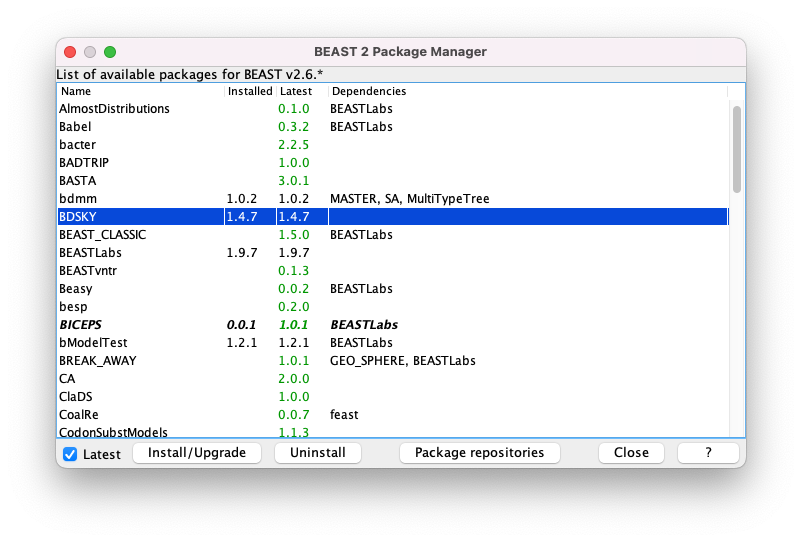
\includegraphics[width=0.750000\textwidth]{figures/install_bdsky.png}
    \caption{Install the BDSKY package which contains the Birth-Death Skyline model.}
    \label{fig:install}
\end{figure}


\subsection{Setting up a Coalescent Bayesian Skyline analysis}

We will set up one analysis file that simultaneously runs the Bayesian skyline model 
on both the Alpha and the background datasets. In the analysis we will assume that 
sequences in both datasets evolve under the same site model, but on 
independent trees with different molecular clock models. 
We will use a GTR model without rate heterogeneity as the site model and 
a simple strict clock as the clock model. 

\begin{framed}

  \subsubsection*{Importing the alignments}

  BEAUti should already be open on the \textbf{partitions} tab. 

  \begin{itemize}
    \item Load both alignments (\lstinline!alpha.fas! and \lstinline!background.fas!)
          and set the data type to \textbf{nucleotide} for both. Don't split either 
          dataset into any partitions!
    \item Link the \textbf{Site} models, but leave the \textbf{Clock} and \textbf{Tree} models unlinked.
    \item Rename the shared \textbf{Site Model} to \lstinline!site!.
  \end{itemize}


  \subsubsection*{Sampling dates}

  Select the \textbf{Tip Dates} tab.

  \begin{itemize}
    \item Select the \textbf{alpha} partition and check the \textbf{Use tip dates} option.
    \item Set \textbf{Dates specified} to the \lstinline!as dates with format! option. 
    \item Select \lstinline!yyyy-M-dd! from the dropdown box. 
    \item Click the \textbf{Auto-configure} button. A window will appear where you can specify how BEAUti can find the collection dates in the sequence headers.
    \item Select \textbf{use everything} and specify \textbf{after last \textbar{}} and click \textbf{OK}.
  \end{itemize}

  Now repeat the steps above for the \textbf{background} partition. (You can also clone the settings 
  as you would for a Site Model, but this doesn't work perfectly and you would still need to make 
  some manual changes). 


  \subsubsection*{Site model}

  Select the \textbf{Site Model} tab and select \textbf{GTR} in the \textbf{Subst Model} drop-down menu.
  Make sure that the \textbf{Substitution Rate} is not being estimated and that the \textbf{Gamma Category Count} is set to 0.

  \subsubsection*{Clock model}
  Select the \textbf{Clock Model} tab and check that the clock model is set to \textbf{Strict Clock} for 
  both partitions.

\end{framed}

Next, we will select the coalescent Bayesian Skyline plot as the tree prior for both trees. 

\begin{framed}
  Select the \textbf{Priors} tab.

  Select \textbf{Coalescent Bayesian Skyline} in the drop-down menus next to \textbf{Tree.t:alpha} and 
  \textbf{Tree.t:background}.

\end{framed}

By default the skyline model has a dimension of 5, meaning that the period between the time of the most 
recent common ancestor (tMRCA) and the most recent sequence is divided into 5 intervals or segments. 
We would like to set the dimension to 10, to allow some more flexibility. 

\begin{framed}
To change the dimensions of parameters we have to navigate to the
\textbf{Initialialization} panel, which is by default not visible.
Navigate to \textbf{View \textgreater{} Show Initialization Panel} to
make it visible and navigate to it (Figure \ref{fig:init}).

Set the dimensions of \textbf{bPopSizes.t:alpha}, \textbf{bGroupSizes.t:alpha}, 
\textbf{bPopSizes.t:background} and \textbf{bGroupSizes.t:background} to 10 each.
(the default value is 5) (Figure \ref{fig:dimensions}).

\end{framed}

\begin{figure}
    \centering
    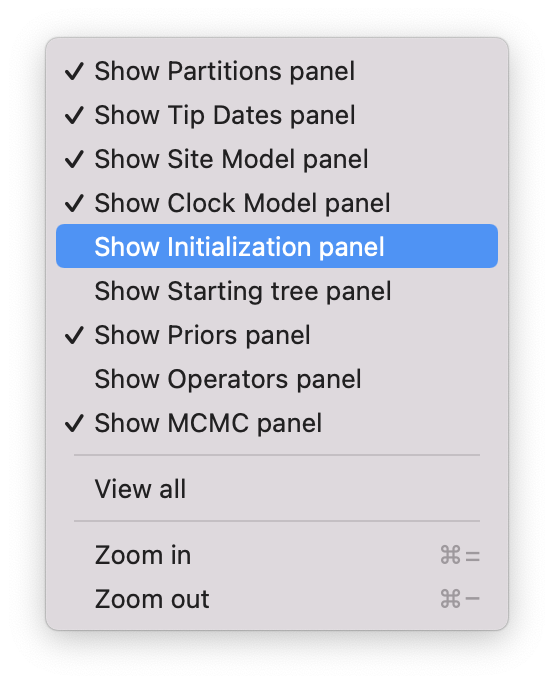
\includegraphics[width=0.250000\textwidth]{figures/goto_initialization.png}
    \caption{Show the initialization panel.}
    \label{fig:init}
\end{figure}

\begin{figure}
    \centering
    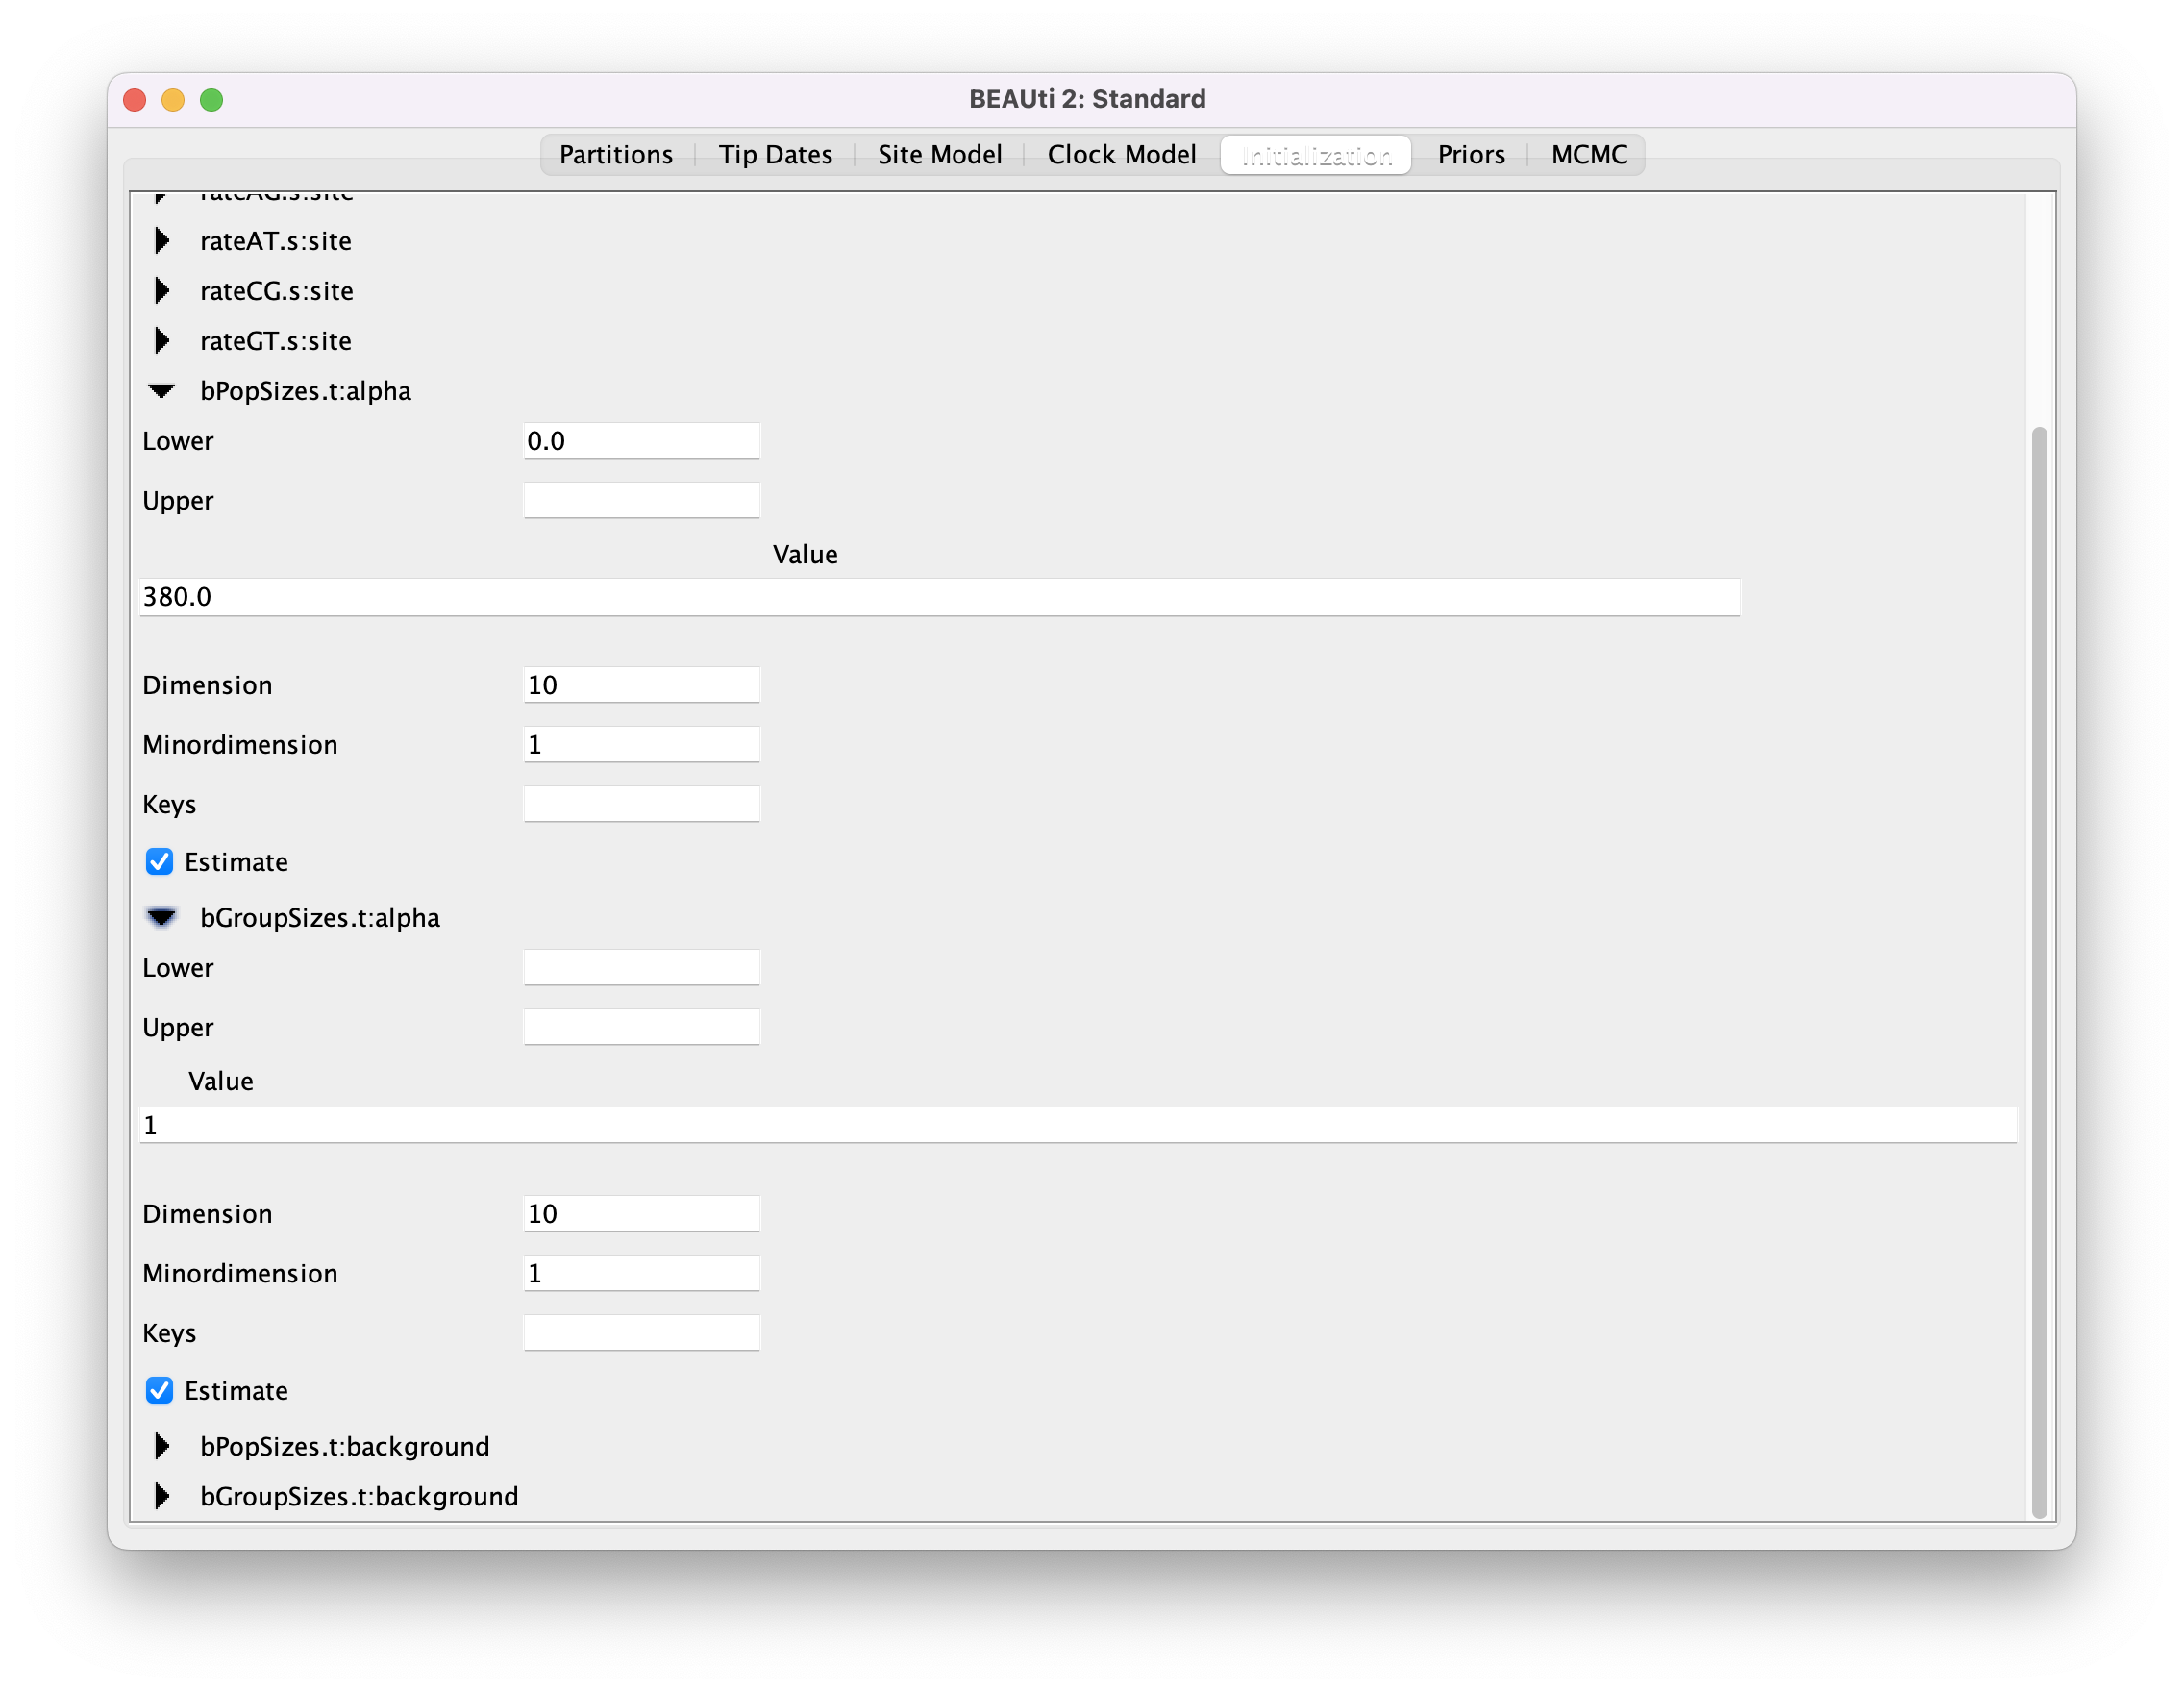
\includegraphics[max width=\textwidth, max height=0.9\textheight]{figures/set_dimension_bsp.png}
    \caption{Set the dimension of bPopSizes and bGroupSizes to 10 (remember to do this for both trees).}
    \label{fig:dimensions}
\end{figure}

Next, we will set a more appropriate prior for the clock rate.

\begin{framed}
    For \textbf{clockRate.c:alpha} select \textbf{Log Normal} from the drop-down
    menu

    \begin{itemize}

    \item
      Expand the options for \textbf{clockRate.c:clock} using the arrow
      button on the left.
    \item
      Set the \textbf{M} parameter to \textbf{5E-4}.
    \item
      Set the \textbf{S} parameter to \textbf{0.2}
    \item
      Check the \textbf{Mean in Real Space} box
    \end{itemize}

    Now repeat the steps above for \textbf{clockRate.c:background}.
\end{framed}

The BEAUti panel should look as shown in Figure \ref{fig:priors}.

\begin{figure}
    \centering
    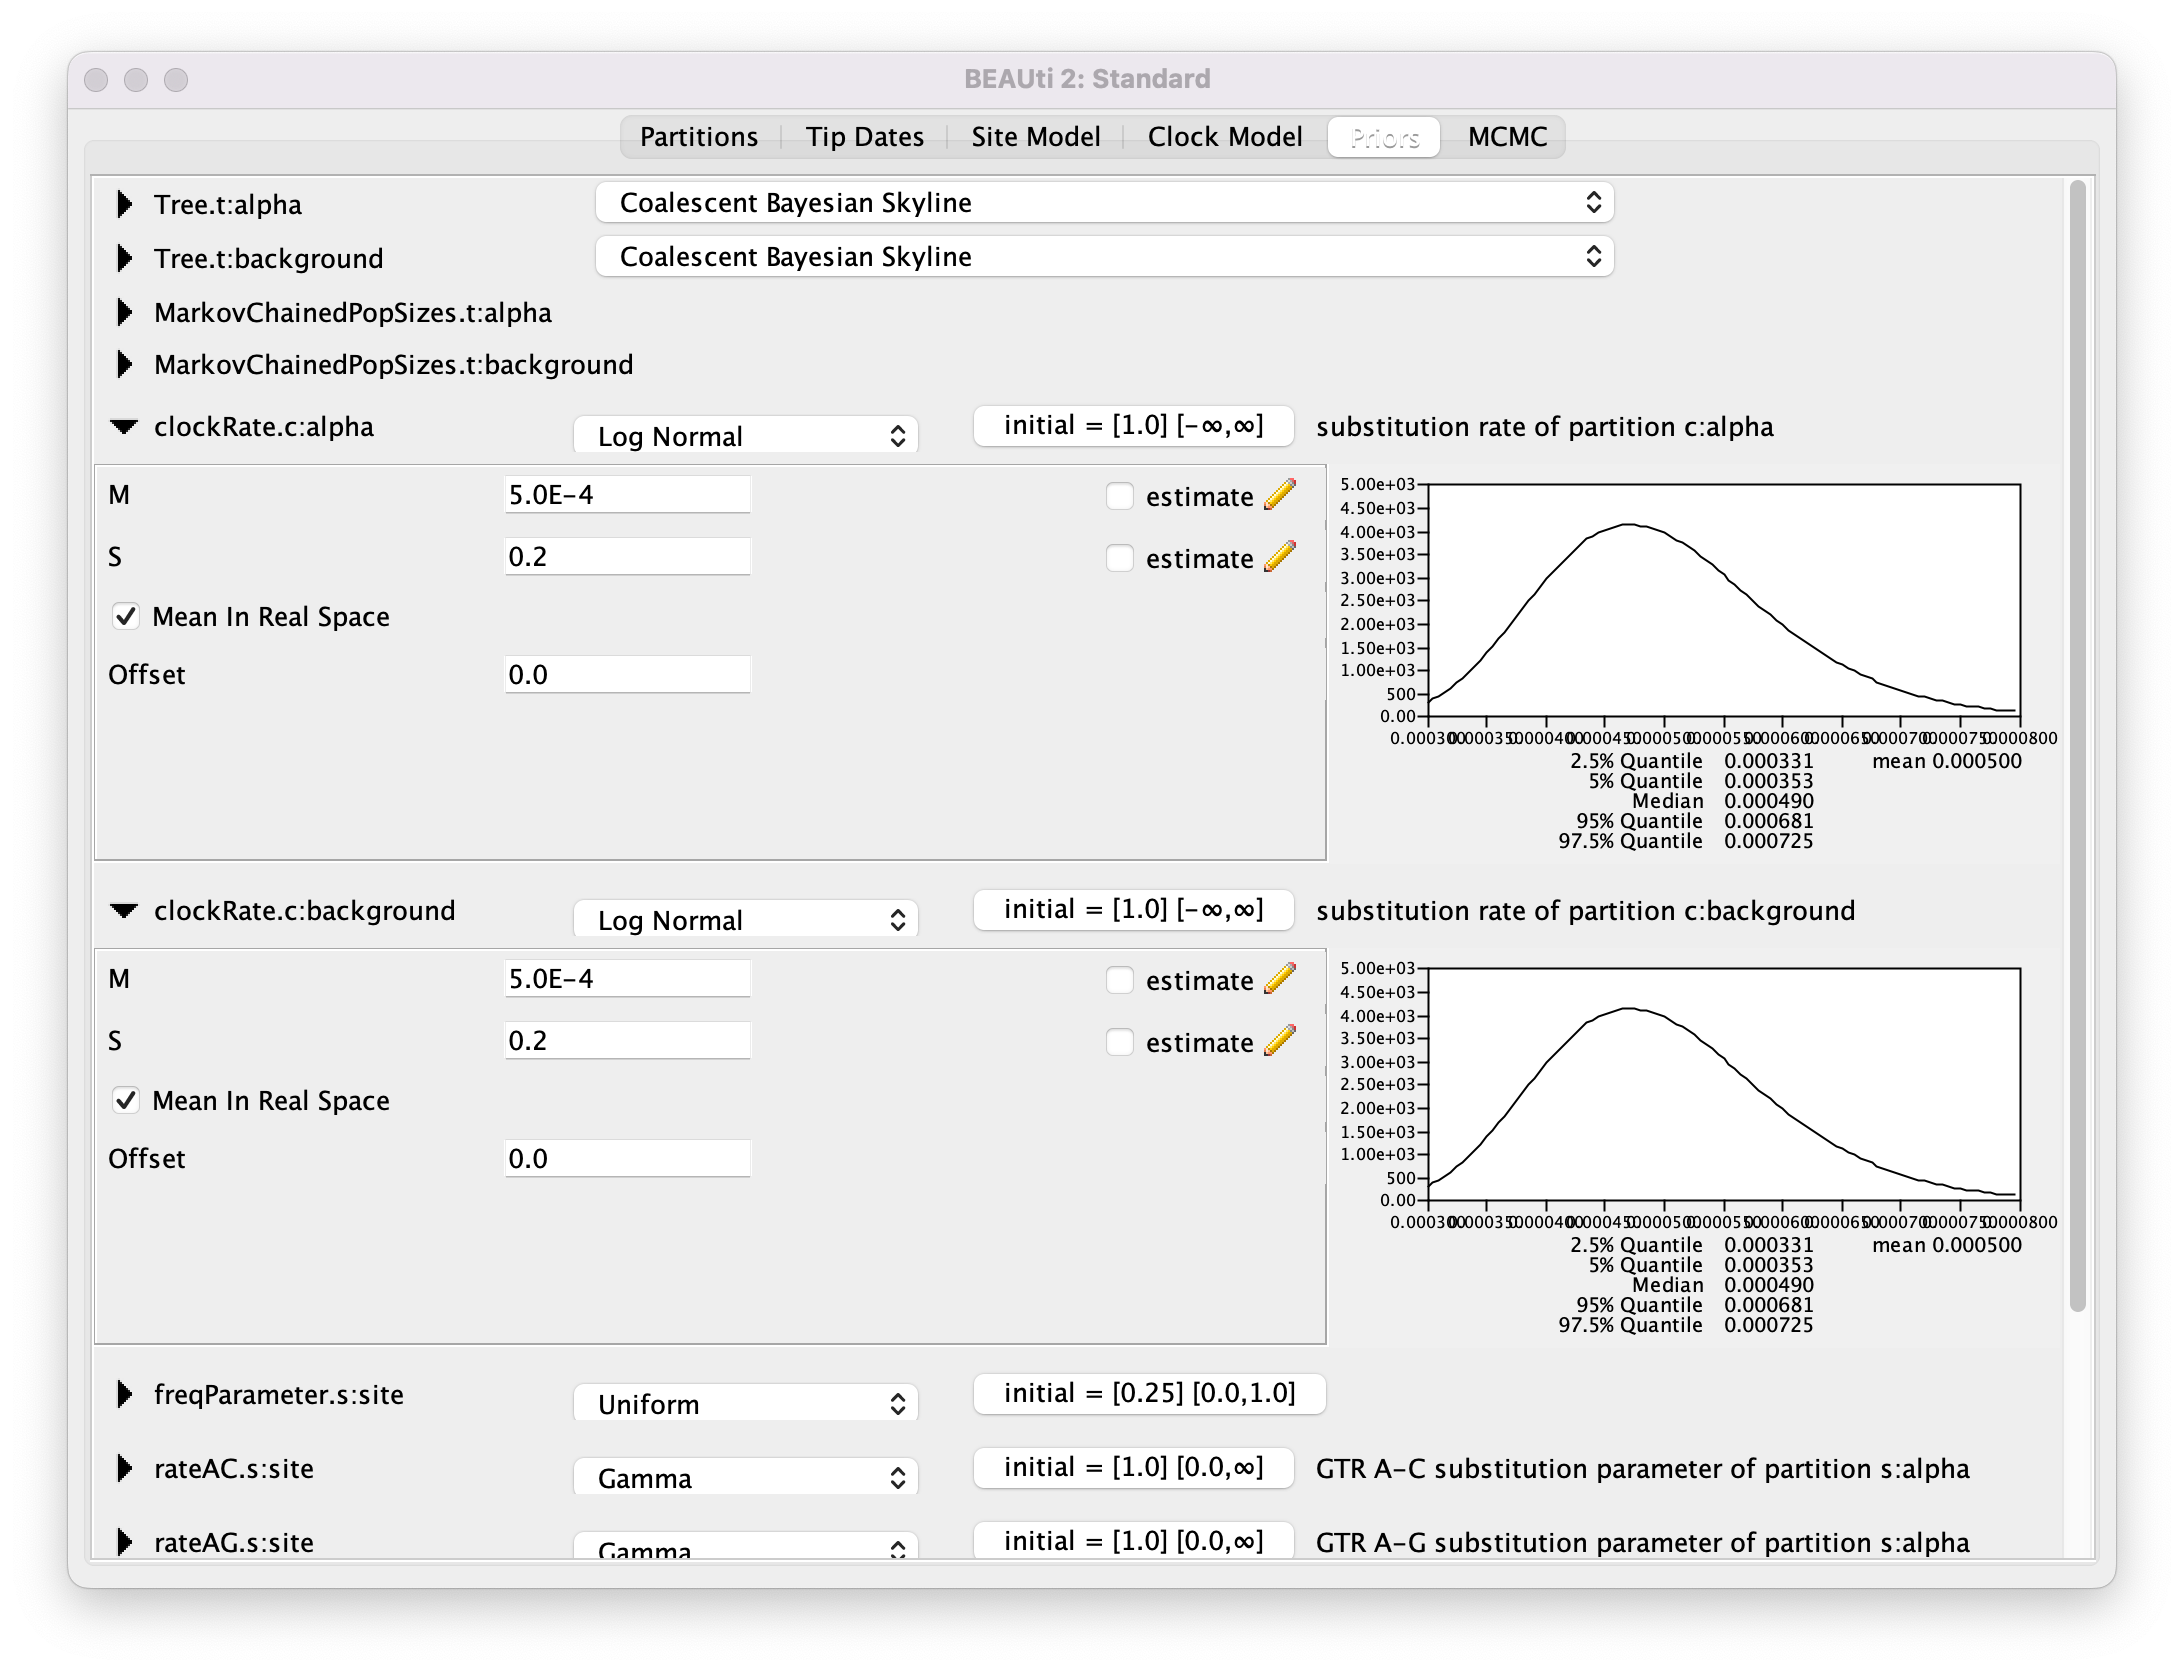
\includegraphics[max width=\textwidth, max height=0.9\textheight]{figures/priors_bsp.png}
    \caption{Prior setup.}
    \label{fig:priors}
\end{figure}

Finally, we will set the MCMC settings and the output file names.

\begin{framed}
  Go to the \textbf{MCMC} tab.

  \begin{itemize}
      \item Set the \textbf{Chain Length} to \textbf{10'000'000}.
      \item Expand the \textbf{tracelog} options, change the \textbf{File Name} to 
            \lstinline!$(filebase)_$(seed).log! and set the 
            \textbf{Log Every} parameter to \textbf{1000}.
      \item Expand the \textbf{screenlog} options and set the 
            \textbf{Log Every} parameter to \textbf{10'000}.
      \item Expand the \textbf{treelog.t:alpha} options, change the \textbf{File Name} to 
            \lstinline!$(filebase)_$(tree)! and set the 
            \textbf{Log Every} parameter to \textbf{1000}.
      \item Expand the \textbf{treelog.t:alpha} options, change the \textbf{File Name} to 
            \lstinline!$(filebase)_$(tree)! and set the 
            \textbf{Log Every} parameter to \textbf{1000}.
      \item Save the XML file under the name \lstinline!bsp.xml! using 
            \textbf{File \textgreater{} Save}.
  \end{itemize}

\end{framed}



When we run the analysis \lstinline!$(filebase)! in the name of the
\lstinline!*.log! and \lstinline!*.trees! files will be replaced by the
name of the XML file, \lstinline!$(tree)! by the tree parameter names and \lstinline!$(seed)! 
by the random number seed. 
This is a good idea, since it makes it easy to
keep track of which XML files and which random number seeds produced which output files.

When using the coalescent Bayesian Skyline plot it is very important that the \textbf{Log Every}
parameter for the trace and tree log files are set to the same frequency, or else Tracer won't be
able to reconstruct the skyline plot! 

Now we are ready to run the analysis.
Do \textbf{NOT} close BEAUti, as we will return to it in the following sections!

\begin{framed}
Run the \textbf{BEAST2} program.

\begin{itemize}
\item
  Select \lstinline!bsp.xml! as the \textbf{Beast XML File}.
\item
  Set the \textbf{Random number seed} to \textbf{777} (or pick your
  favourite number).
\item
  Check the \textbf{Use BEAGLE library if available} checkbox. If you
  have previously installed BEAGLE this will make the analysis run
  faster.
\end{itemize}

Run \textbf{BEAST2} by clicking the \lstinline!Run! button.
\end{framed}

The analysis will take some time to complete (allow at least 15-20 minutes). Read through the
next section while waiting for your results or start preparing the XML
file for the \protect\hyperlink{sec:bdsky}{birth-death skyline}
analysis.

\subsection{The Coalescent Bayesian Skyline
parameterization}\label{the-coalescent-bayesian-skyline-parameterization}

The Kingman coalescent model that the Coalescent Bayesian Skyline is based on
assumes that the sequences represent a small sample from a haploid
population evolving under Wright-Fisher dynamics (Figure
\ref{fig:wrightfisher}). The model works by calculating the probability
of the tree under this assumption. This essentially boils down to
repeatedly asking the question of how likely it is for two lineages to
coalesce (have a common ancestor) in a given time.

\begin{figure}
    \centering
    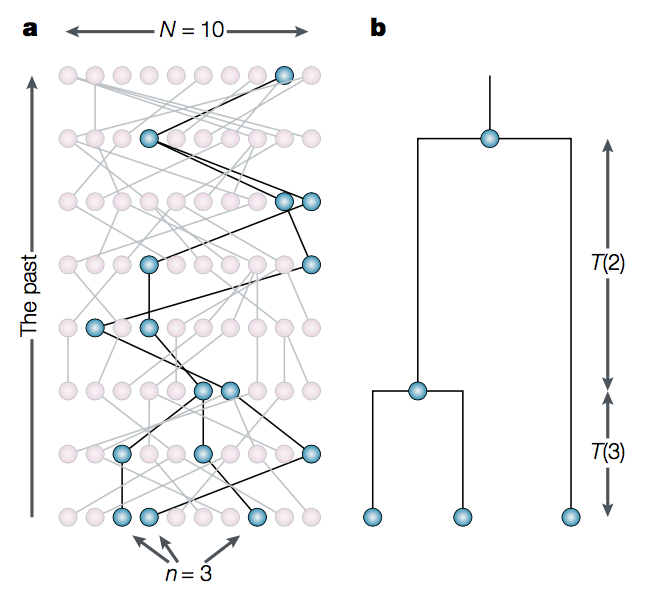
\includegraphics[width=0.500000\textwidth]{figures/Rosenberg2002.png}
    \caption{The basic principle behind the coalescent. Figure from \citep{Rosenberg2002}.}
    \label{fig:wrightfisher}
\end{figure}

The effective population size ($ N_e $) is the inverse of
the rate of coalescence $ \lambda $. The larger
$ N_e $ is, the less likely lineages are to coalesce. Thus,
intervals in a sampled tree with many branching events often coincide
with periods when the population size was small. Similarly, few
branching events occur during periods of large population size. (Note
that these results are conditioned on sampling only a small fraction of
the population).

\begin{equation}
    \lambda = \frac{1}{N_e}
\end{equation}

For an SIR model (\textbf{S}usceptible, \textbf{I}nfected and
\textbf{R}ecovered), $ N_e $ is proportional to the overall
population size $ N $ and the number of infected
$ I $ and inversely proportional to the transmission rate
$ \theta $.

\begin{equation}
    N_e = \frac{I}{\theta} \frac{N}{S}
\end{equation}

Estimates of $ N_e $ therefore do not directly tell us
something about the number of infected, nor the transmission rate.
However, changes in $ N_e $ can be informative about changes
in the transmission rate or the number of infected (if they do not
cancel out).

\begin{figure}
    \centering
    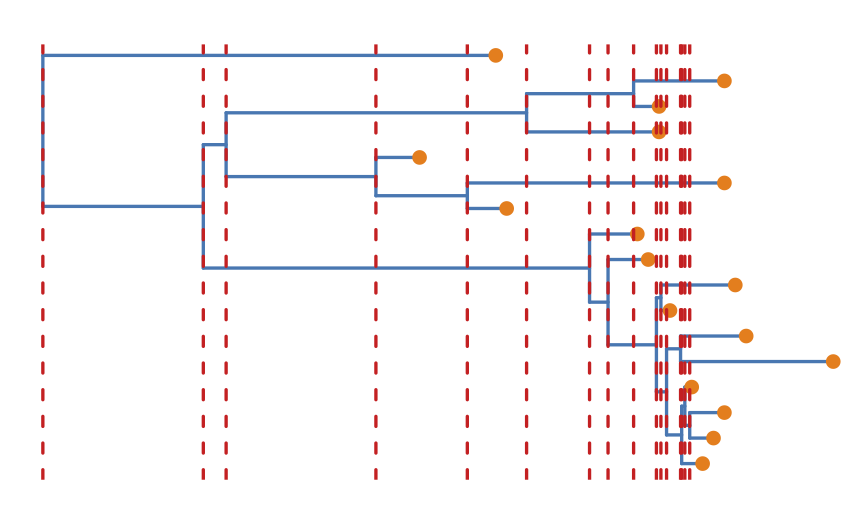
\includegraphics[width=0.750000\textwidth]{figures/coalescent_intervals.png}
    \caption{Example tree where the red dotted lines show the time-points of coalescent events.}
    \label{fig:coal_events}
\end{figure}

The Coalescent Bayesian Skyline model allows $ N_e $ to
change over time in a nonparametric fashion (i.e.~we do not have to
specify an equation governing changes in $ N_e $ over time).
It divides the time between the present and
the root of the tree (the tMRCA) into segments, and estimates a
different effective population size ($ N_e $) for each
segment. The endpoints of segments are tied to the branching times (also
called coalescent events) in the tree (Figure \ref{fig:coal_events}),
and the size of segments is measured in the number of coalescent events
included in each segment. The Coalescent Bayesian Skyline groups
coalescent events into segments and jointly estimates the
$ N_e $ (\textbf{bPopSizes} parameter in BEAST) and the size
(\textbf{bGroupSizes} parameter) of each segment. To set the number of
segments we have to change the dimension of \textbf{bPopSizes} and
\textbf{bGroupSizes} (note that the dimensions of both parameters always have to
be the same). Note that the length of a segment is not fixed, but
dependent on the timing of coalescent events in the tree (Figure
\ref{fig:coal_events}), as well as the number of events contained within
a segment (\textbf{bGroupSizes}).

Another way to think about the model is as maximally-parameterized,
since it infers $ d $ change-point times (segment
boundaries) and a value for $ N_e $ in each segment. This
makes the Bayesian Skyline flexible enough to model very complicated
$ N_e $ dynamics, provided that enough segments are
specified. It may be tempting to specify the maximum dimension for the
model (each group contains only one coalescent event, thus
$ N_e $ changes at each branching time in the tree), making
it as flexible as possible. This is the parameterization used by the
Classic Skyline plot \citep{Pybus2000}, which is the direct ancestor of
the Coalescent Bayesian Skyline plot. However, the only informative
events used by the Coalescent Bayesian Skyline plot are the coalescent
events. Thus, using a maximally-flexible parameterization with only one
informative event per segment often leads to erratic and noisy estimates
of $ N_e $ over time (especially if segments are very short). 
Grouping segments together leads to
smoother and more robust estimates.

Choosing the dimension for the Bayesian Skyline can be rather arbitrary.
If the dimension is chosen too low, not all population size changes are
captured, but if it is chosen too large, there may be too little
information in a segment to support a robust estimate. When trying to
decide if the dimension is appropriate it may be useful to consider the
average number of informative (coalescent) events per segment. (A tree
of $ n $ taxa has $ n-1 $ coalescences, thus
$ N_e $ in each segment is estimated from on average
$ \frac{n-1}{d} $ informative data points). Would this
number of random samples drawn from a hypothetical distribution allow
you to accurately estimate the distribution? If not, consider decreasing
the dimension. There are descendants of the coalescent skyline in BEAST
that either estimate the number of segments (Extended Bayesian Skyline
\citep{Heled2008}) or do not require the number of segments to be
specified (Skyride \citep{Minin2008} or Skygrid \citep{Gill2013} models), but instead makes very strong
prior assumptions about smoothly how $ N_e $ changes through time.



\subsection{Setting up a Birth Death Skyline analysis}

We will now repeat the analysis using the Birth Death Skyline model. Either set up a new XML file in BEAUti and follow the same steps as above until you've specified the site and clock models or else simply go back to BEAUti and edit the previous analysis file. 

We will need to set the prior to \textbf{Birth Death Skyline
Serial}, since the sequences were sampled at different times. 
For homochronous data (all sequences sampled at the same time), we
would use \textbf{Birth Death Skyline Contemporary}. 

\begin{framed}
  Select the \textbf{Priors} tab.

  Select \textbf{Birth Death Skyline Serial} in the drop-down menus next to \textbf{Tree.t:alpha} and 
  \textbf{Tree.t:background}.

\end{framed}



Note that priors for two \textbf{reproductiveNumber}, \textbf{origin}, \textbf{becomeUninfectiousRate} and \textbf{samplingProportion} parameters have been added to the panel; one set for each tree.
Besides $ R_e $ (\textbf{reproductiveNumber}), the
\textbf{Birth Death Skyline Serial} model has 3 more parameters,
\textbf{becomeUninfectiousRate} (the rate at which infected patients
become uninfectious, $ \delta $, through recovery, death or
isolation), \textbf{samplingProportion} (the proportion of removed lineages during a time period 
that are sampled) and the \textbf{origin} (the time at
which the index case became infected, which is always earlier than the
tMRCA of the tree). We may know some of these parameters from literature
or be able to estimate them from external sources. For example, the
average time that patients are able to transmit a disease is informative
about the \textbf{becomeUninfectiousRate}. This prior knowledge we can
incorporate in our analysis by setting appropriate priors for these
parameters.

As with the Coalescent
Bayesian Skyline, we need to set the number of dimensions. We will set
the dimension of $ R_e $, which denotes the average number of secondary infections caused
by an infected person at a given time during the epidemic, i.e.~an
$ R_e $ of 2 would mean that every infected person causes
two new infections on average. In other words, an $ R_e $
above 1 means that the number of cases are increasing, therefore the
disease will cause an exponentially growing epidemic, and an
$ R_e $ below 1 means that the epidemic will die out.
We will also set the dimension of the \textbf{samplingProportion} parameters, so that we can also estimate
changes in the sampling proportion over time. 

In general, we need to fix one of the rates of the 
birth-death skyline model in order to make the model identifiable, although in some cases 
we can get away with strong priors on all rates.  
Here we will fix the \textbf{becomeUninfectiousRate} to 36.5 for both trees, 
which translates to a mean infected period of 10 days (the inverse of the rate), which 
we know to be a realistic estimate for SARS-CoV-2. 

\begin{framed}

    Navigate to the \textbf{Initialialization} panel.

    \begin{itemize}
      \item Set the dimensions of both \textbf{samplingProportion} parameters to 10.
      \item Double-check that both \textbf{reproductiveNumber} parameters have a dimension of 10.
      \item Uncheck the \textbf{Estimate} checkboxes after expanding the options for both 
            \textbf{becomeUninfectiousRate} parameters. As soon as you uncheck the box they will 
            disappear from the panel! 
    \end{itemize}

    You could also change the dimension of parameters in the \textbf{Priors} tab.
    In the \textbf{Priors} tab, click on the button where it says \textbf{initial = {[}2.0{]}
    {[}0.0, Infinity{]}} next to \textbf{reproductiveNumber\_BDSKY\_...}. A pop-up
    window will open which allows us to change the dimension of the
    parameter (Figure~\ref{fig:dimensions_bdsky}).

\end{framed}


\begin{figure}
    \centering
    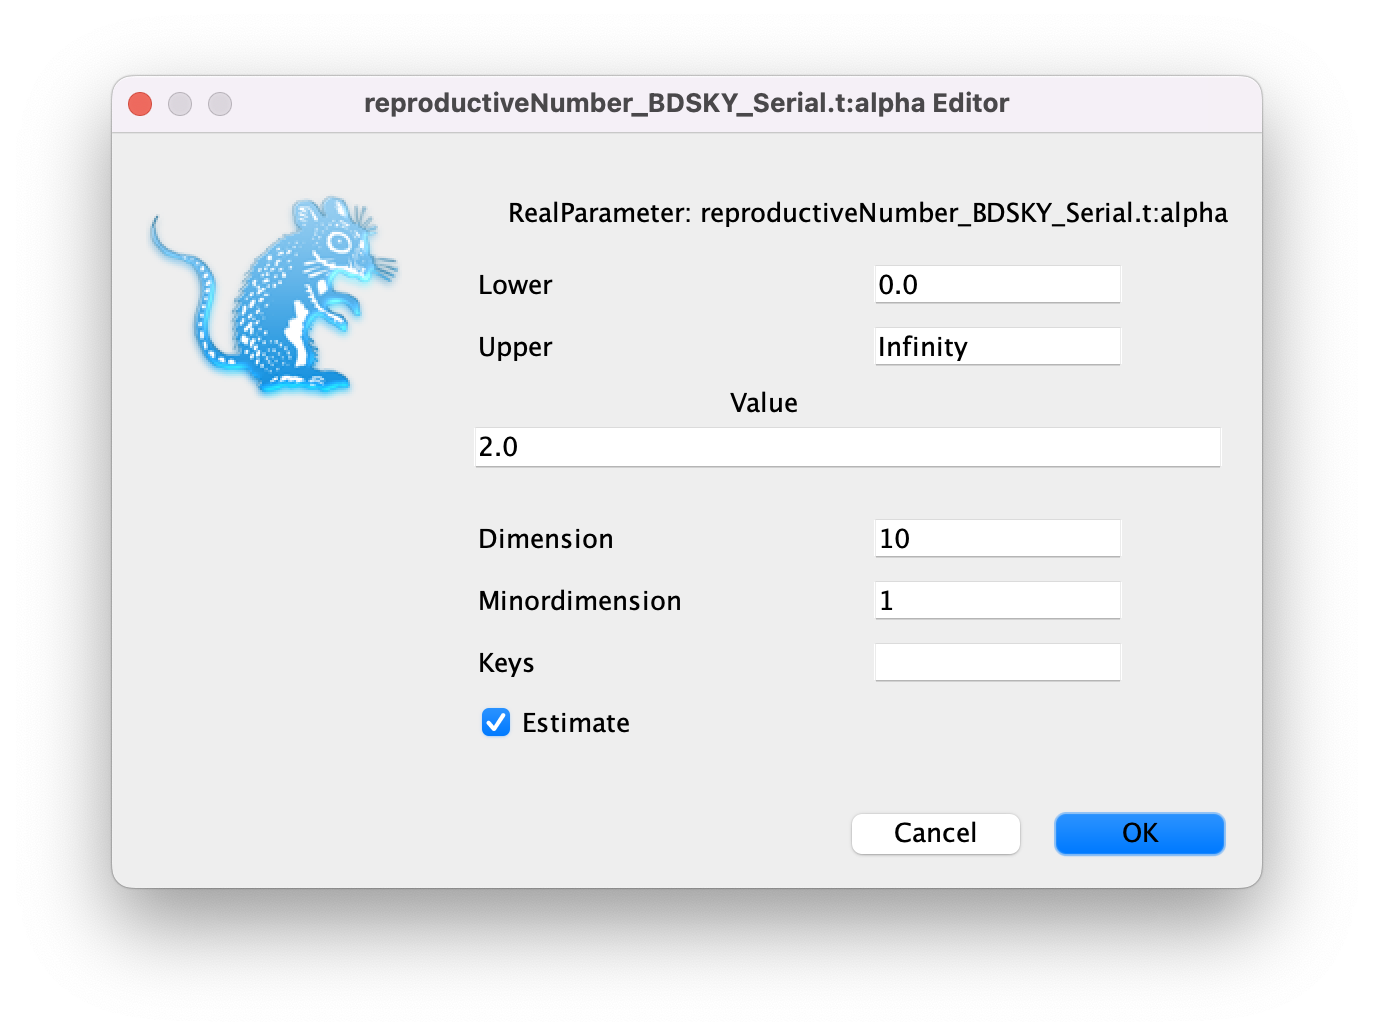
\includegraphics[width=0.750000\textwidth]{figures/choose_dimension_bdsky.png}
    \caption{Setting the dimension of the reproductiveNumber parameter.}
    \label{fig:dimensions_bdsky}
\end{figure}

Now $ R_e $ and the sampling proportion will be allowed to change at 9 times
equally spaced between the origin of the epidemic and the time of the most recent sample, in 
our case March 1st, 2021.
Choosing this dimension can be arbitrary and may require the
testing of a few different values. Too few intervals and not all rate
shifts are captured. Too many intervals and the intervals may not
contain enough information to infer parameters. We still need to set the \textbf{becomeUninfectiousRate}
parameters to 36.5.


\begin{framed}
  Return to the \textbf{Priors} tab. 

  \begin{itemize}
    \item Expand the options for \textbf{Tree.t:alpha}.
    \item Enter \textbf{36.5} for \textbf{Become Uninfectious Rate} (Figure~\ref{fig:set_delta}).
  \end{itemize}

  Now repeat the above steps for \textbf{Tree.t:background}.
\end{framed}

\begin{figure}
    \centering
    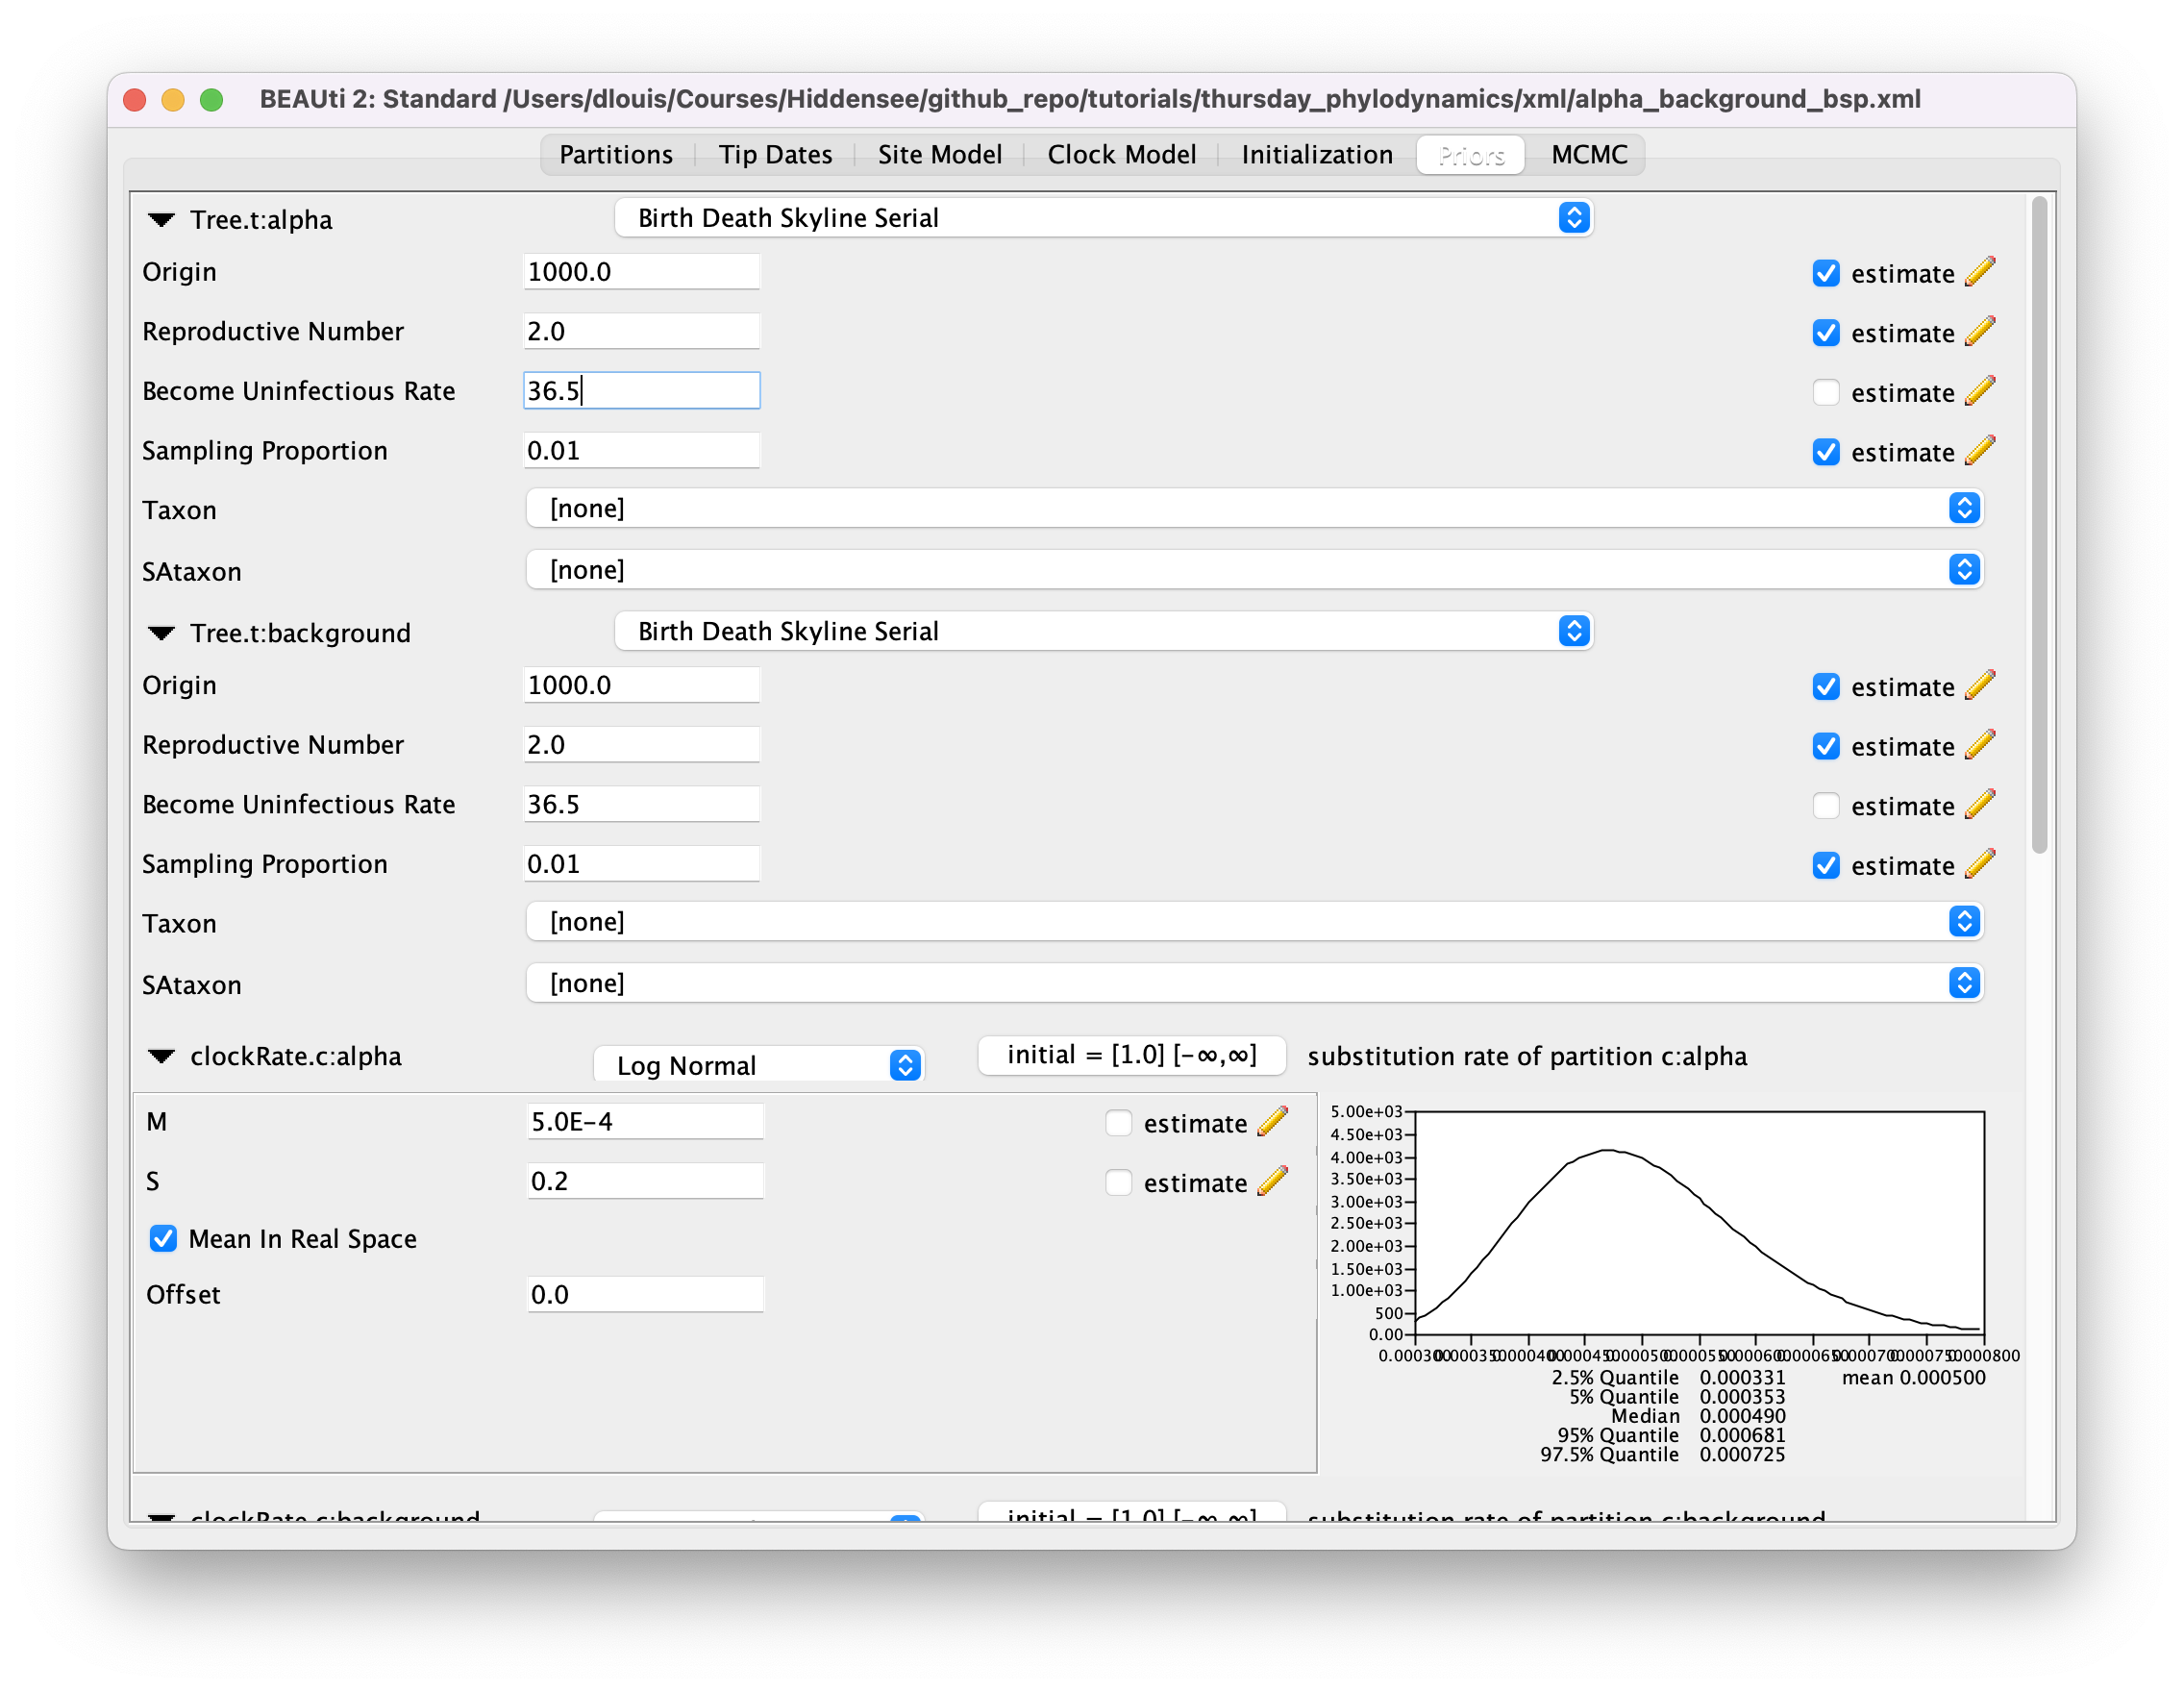
\includegraphics[max width=\textwidth, max height=0.9\textheight]{figures/set_delta.png}
    \caption{Fixing the become uninfectious rate.}
    \label{fig:set_delta}
\end{figure}

We will use a lognormal prior for $ R_e $. This is a good
prior distribution to use for rates since it is always positive (a rate
cannot be negative) and has a long tail defined over all positive
numbers. The long tail allows arbitrarily high estimates of
$ R_e $, but does not place much weight on very high rates.
This agrees with our prior knowledge about $ R_e $ (most
diseases have an $ R_e $ between 1.2 and 8. Measles is one
of the most infectious diseases we know of and has
$ R_e \approx 18 $). 


\begin{framed}
  Select a \textbf{Log Normal} distribution for the first
  \textbf{reproductiveNumber\_BDSKY\_...} prior.

  Click on the arrow to expand the options and set \textbf{M} to 0.8 and \textbf{S} to 0.5.

  Now repeat the above steps for the second \textbf{reproductiveNumber\_BDSKY\_...} 
  parameter  (Figure~\ref{fig:reprior}.
\end{framed}

\begin{figure}
    \centering
    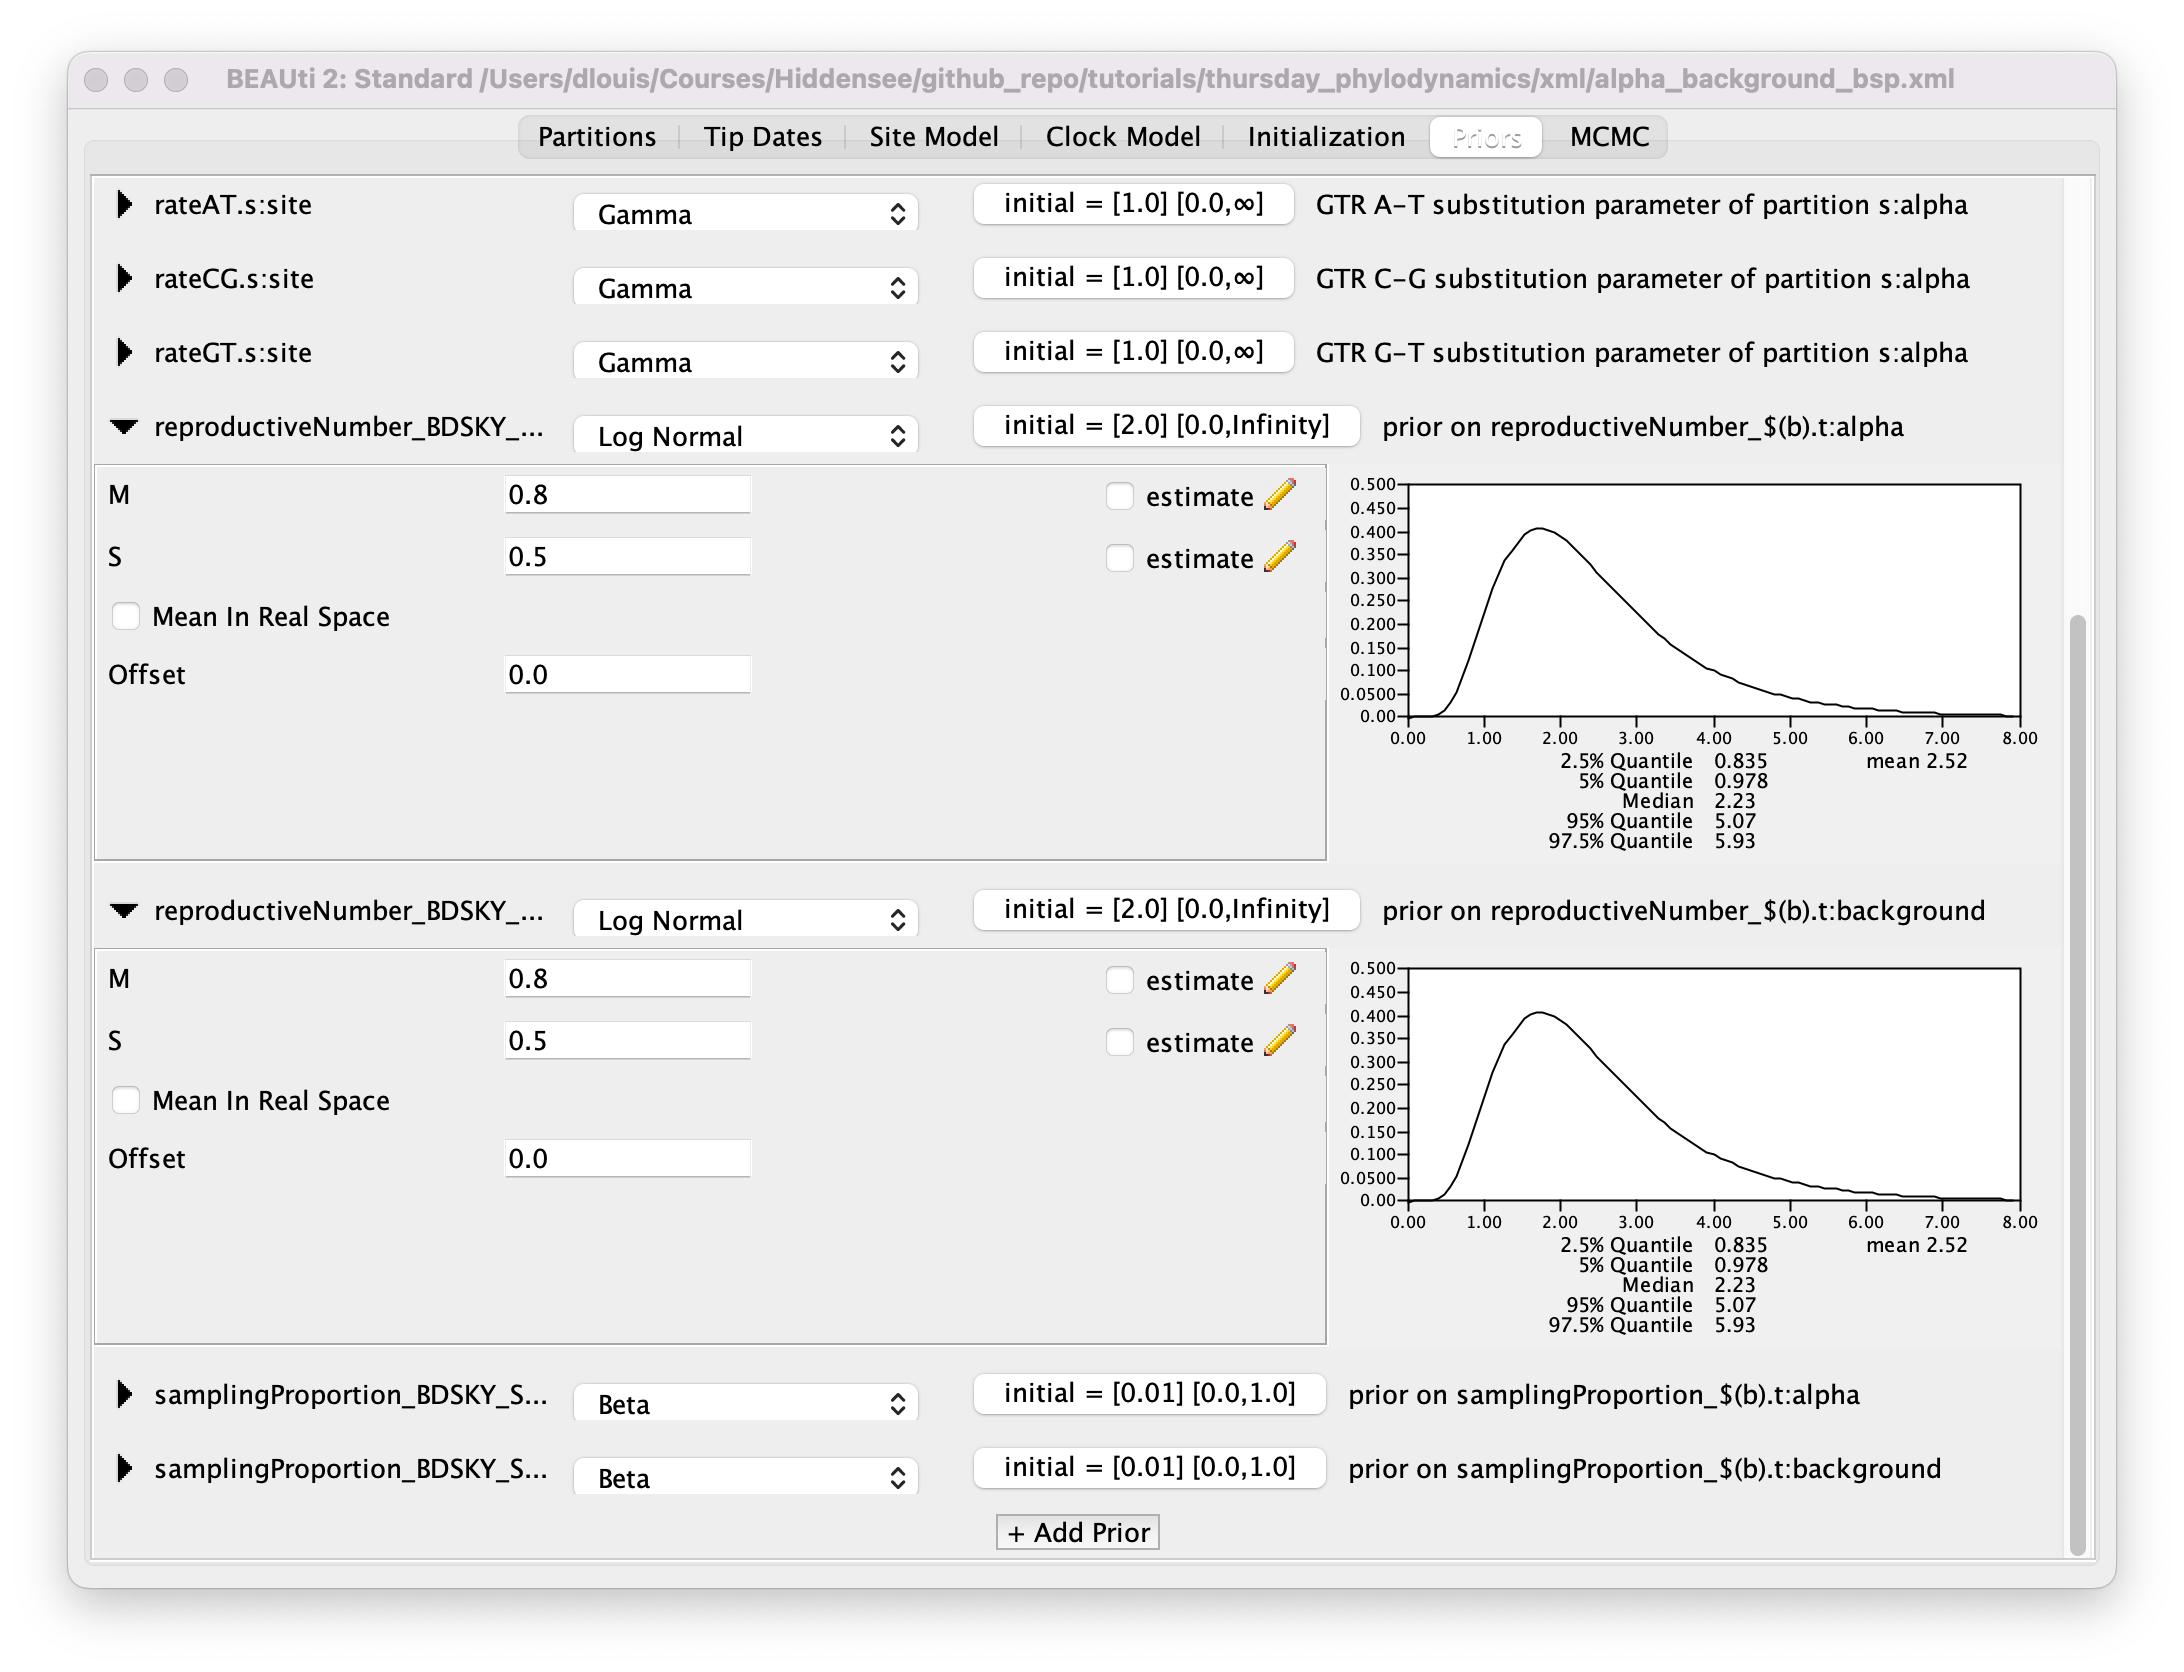
\includegraphics[max width=\textwidth, max height=0.9\textheight]{figures/bdsky_prior_re.png}
    \caption{Setting the `$ R_e $` priors.}
    \label{fig:reprior}
\end{figure}

This prior has a median above 1 and places most of the weight below 5. This agrees with what we 
know of the SARS-CoV-2 epidemic in the UK during the second half of 2020 and the start of 2021, 
when cases grew with the second and third waves of the epidemic. Note that this prior is used for
each of the $ R_e $ intervals (the Birth-Death Skyline
assumes that $ R_e $ is independent in each of the
intervals).

The sampling proportion represents the proportion of removed lineages during 
each interval that were sequenced (included in the alignment).
We will use a Beta distribution for the sampling proportion prior.
Beta distributions are a very flexible class of distributions that are
only defined between 0 and 1, making them well-suited to use for proportions.
A Beta distribution can be interpreted as modelling the probability of success,
out of a number of trials, which is ideal for a sampling model. 
To decide which parameter values to use for the Beta distribution you can 
think of $\alpha - 1$ as the number of successes (cases that were sequenced/observed) 
and $\beta - 1$ as the number of failures (cases that were not sequenced/observed). 


\begin{framed}
Select a \textbf{Beta} distribution for the first \textbf{samplingProportion\_BDSKY\_S...} prior.

Click on the arrow expand the options and set \textbf{Alpha} to \textbf{2} and \textbf{Beta} to 
\textbf{1000} (Figure~\ref{fig:samplingprior}).

Now repeat the above steps for the second \textbf{samplingProportion\_BDSKY\_S...} prior.
\end{framed}


\begin{figure}
    \centering
    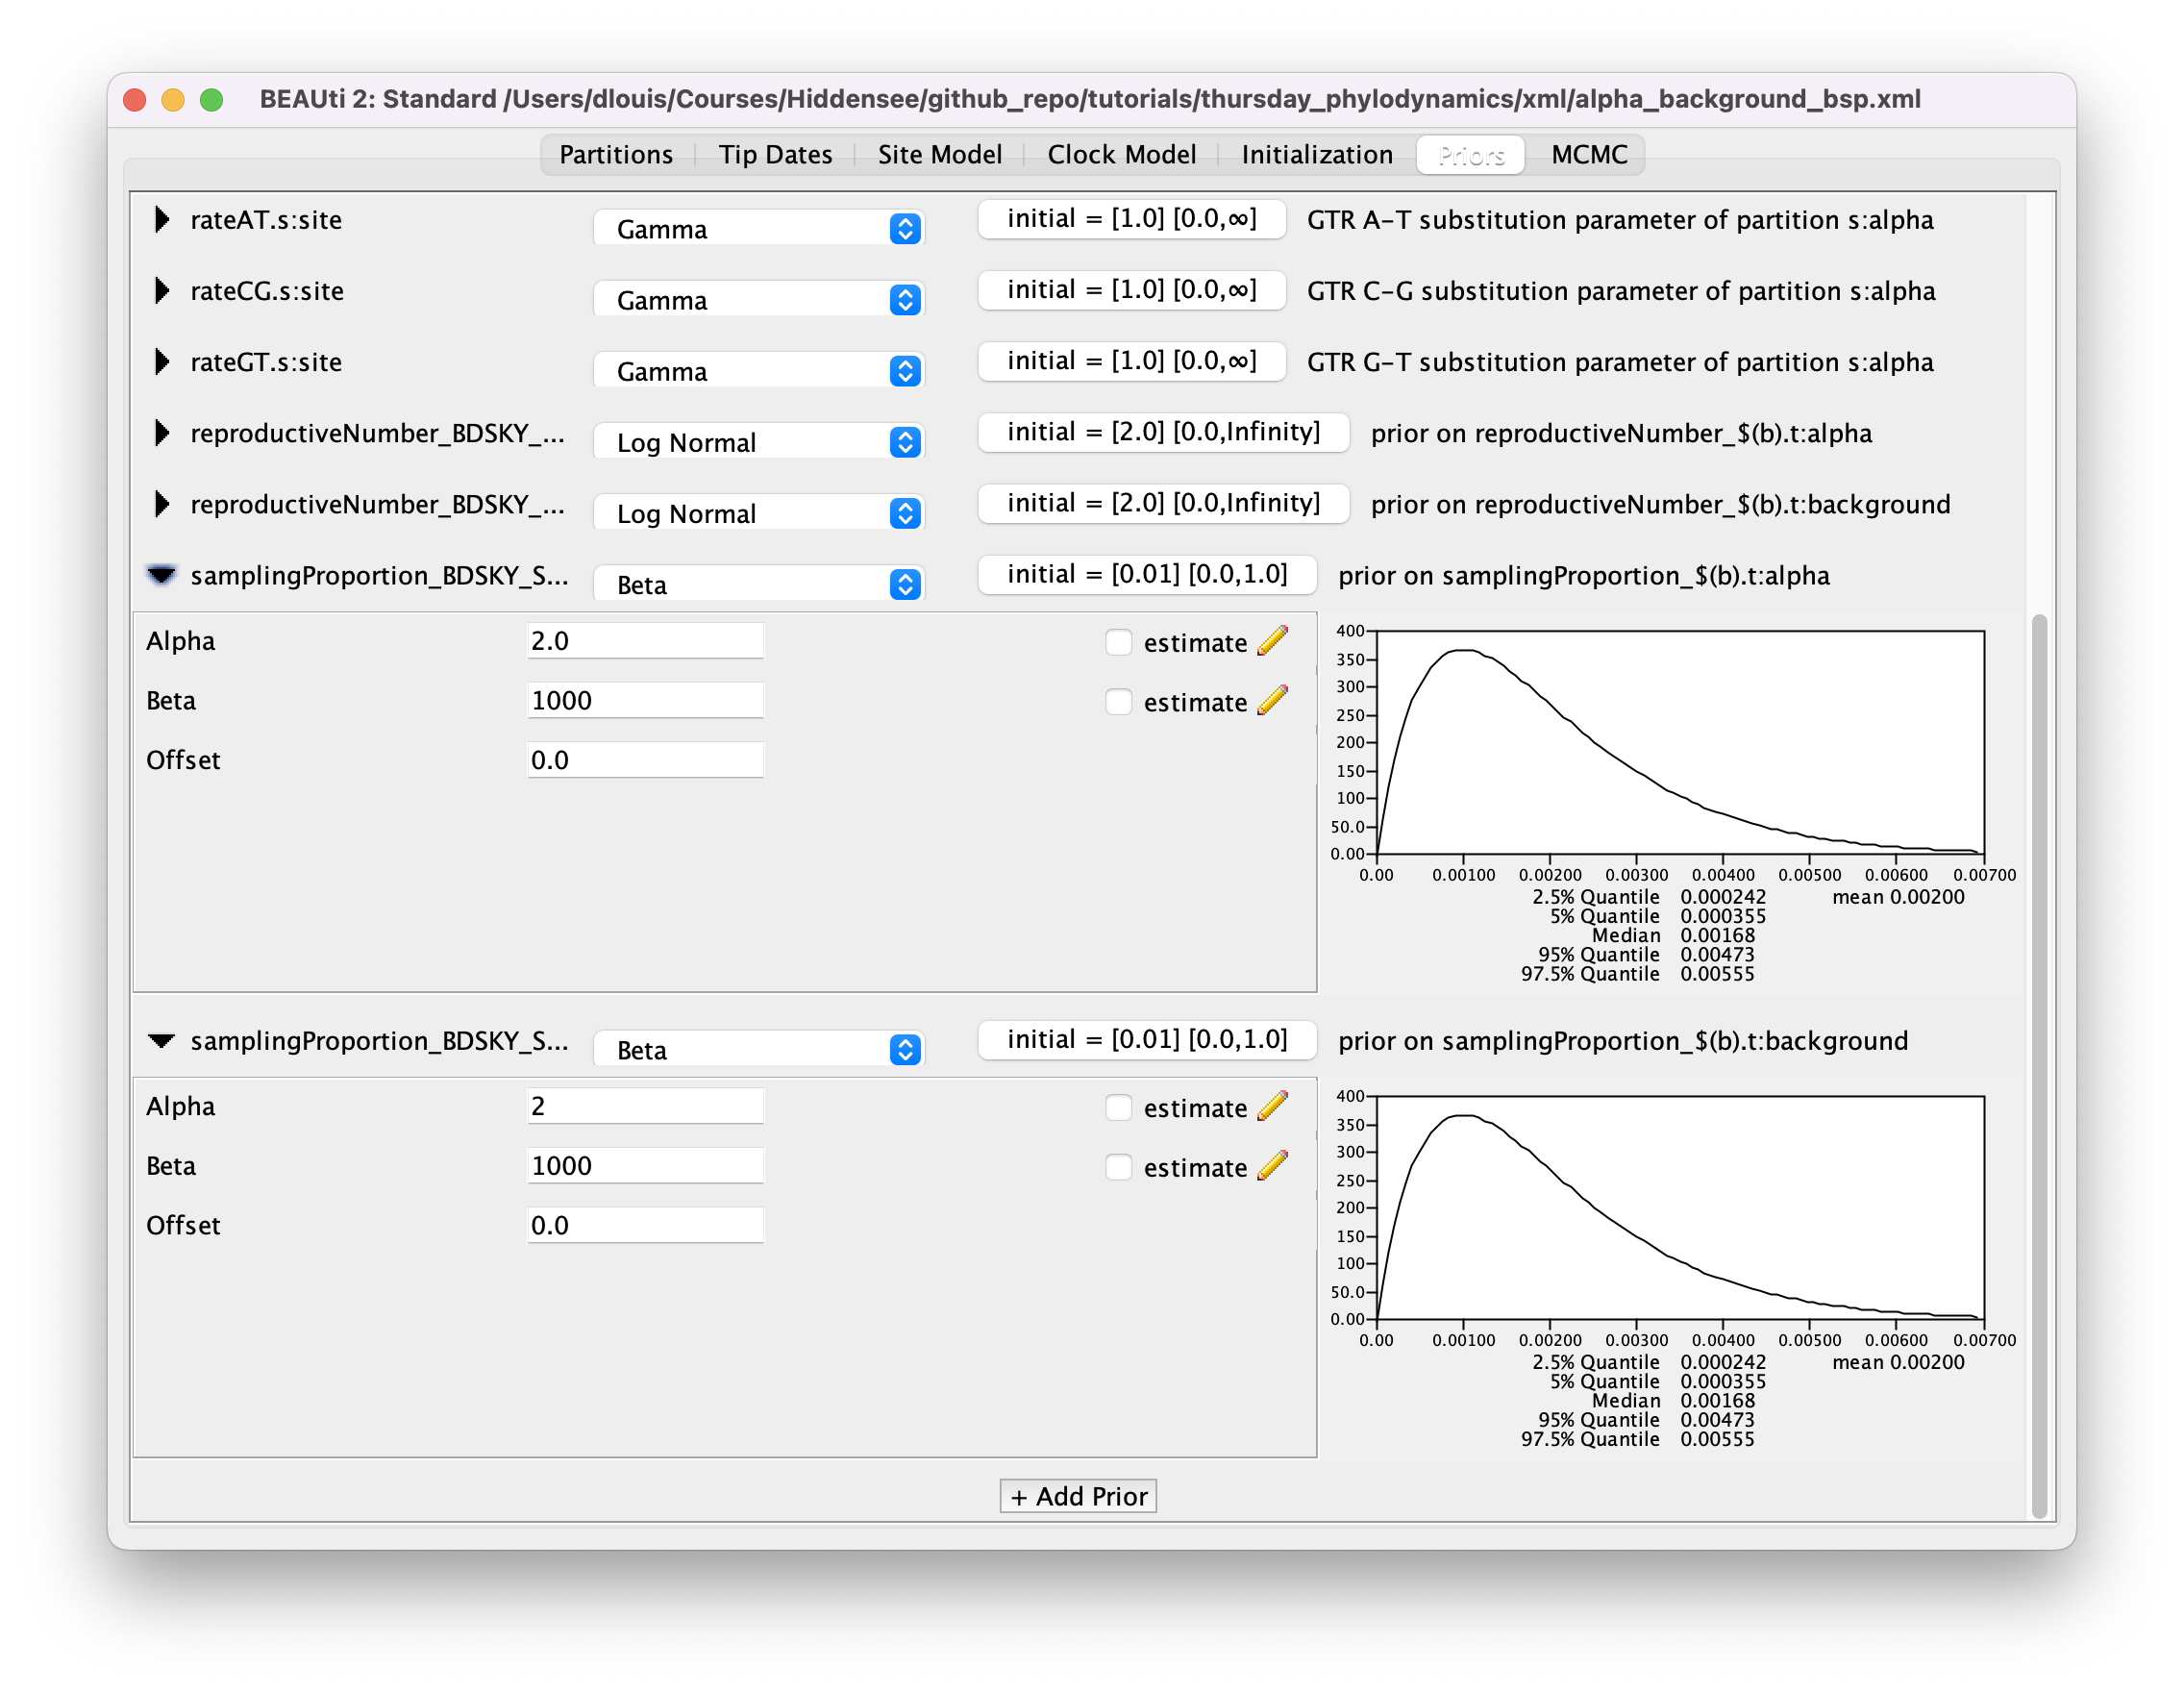
\includegraphics[max width=\textwidth, max height=0.9\textheight]{figures/bdsky_prior_sampling.png}
    \caption{Setting the sampling proportion priors.}
    \label{fig:samplingprior}
\end{figure}

Thus, the prior we set assumes we are sequencing roughly 1 out of every 1000 cases (the distribution 
has a median probability of sequencing a removed lineage of 0.000168). 

Finally, we need to set a prior for the origin of the epidemic. We will
once again use a log normal distribution for this parameter. Note that
the origin also has to be positive and needs to be bigger than the MRCA
of the tree. At this point in the COVID-19 pandemic it had only been circulating 
for a little more than a year, thus we want to set a prior that reflects
this knowledge. Keep in mind that the origin of the Alpha alignment would be
the index case of the Alpha VOC and not of SARS-CoV-2! Similarly, the origin of
the background alignment would be the index case that lead to all genomes 
represented in the dataset, which may not be the same as the index case of the 
entire pandemic. 

\begin{framed}
Set a \textbf{Log Normal} prior for both \textbf{origin} parameters with \textbf{M = -0.5}
and \textbf{S = 0.2} (Figure \ref{fig:originprior}). 
\end{framed}

\begin{figure}
    \centering
    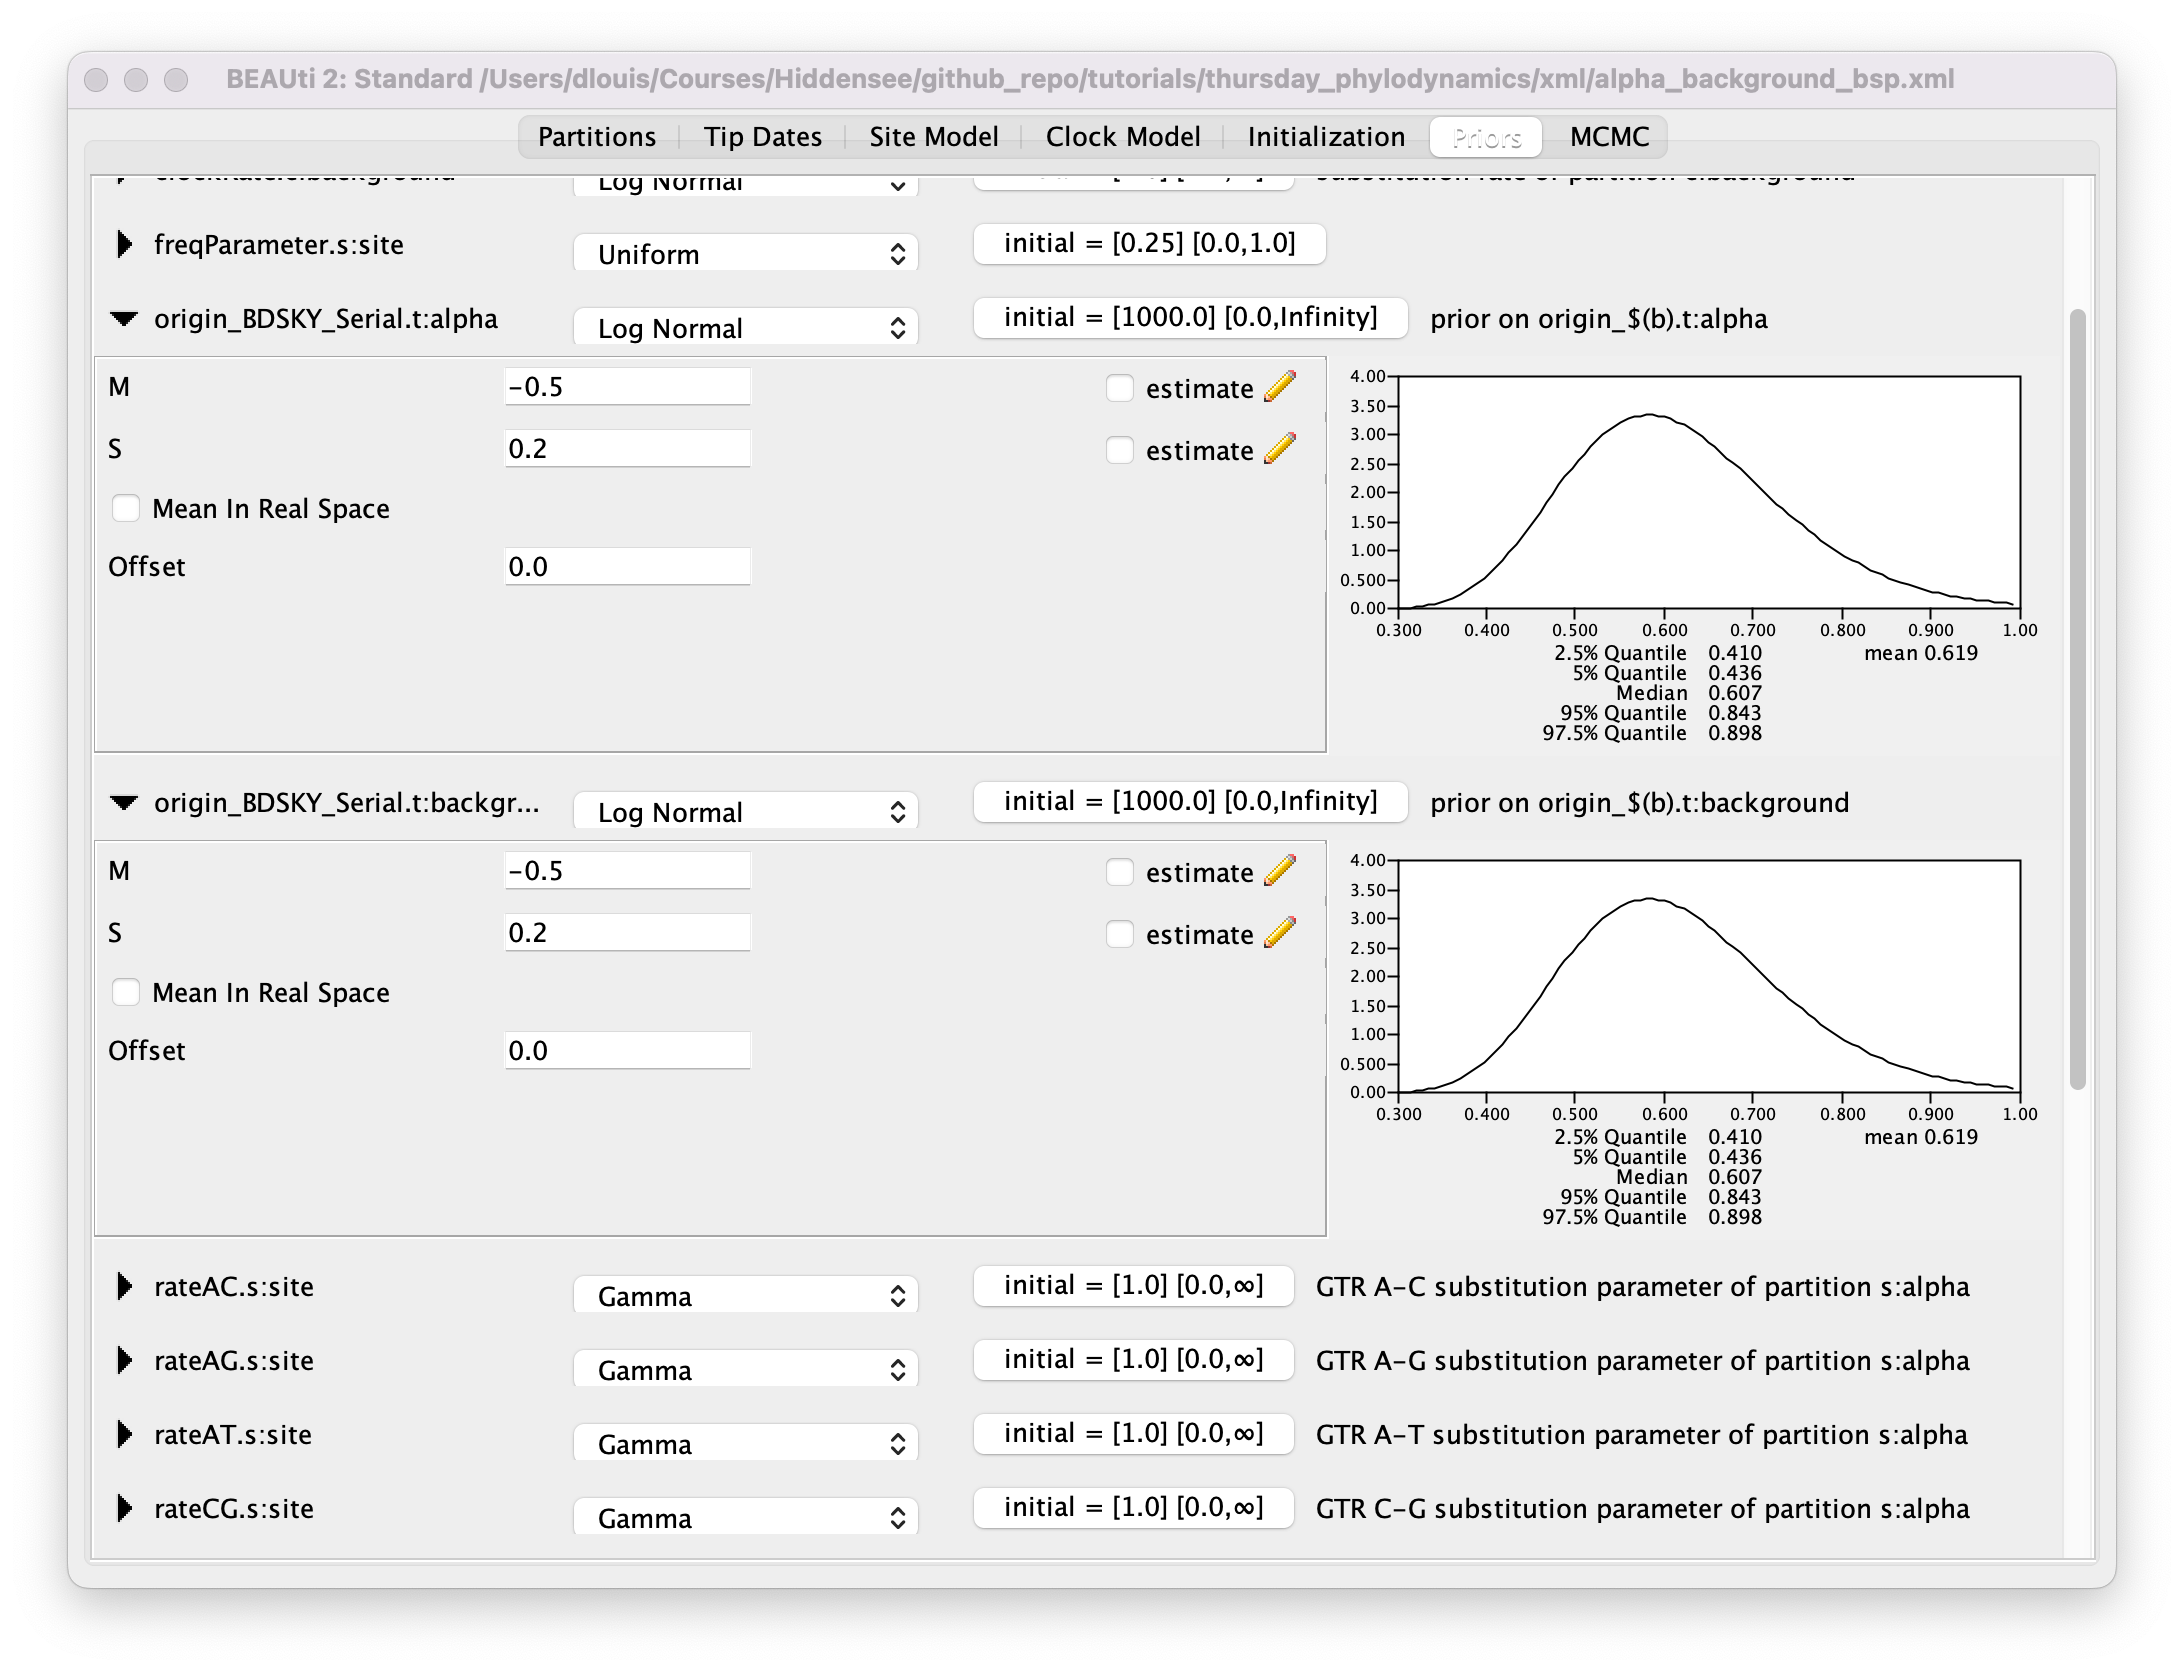
\includegraphics[max width=\textwidth, max height=0.9\textheight]{figures/bdsky_prior_origin.png}
    \caption{Setting the priors on the origins of the epidemics.}
    \label{fig:originprior}
\end{figure}

Double-check that the clock rate priors are the same as those set earlier for the 
coalescent Bayesian Skyline plot.
The rest of the priors pertain to the site model parameters and we can
leave them as they are.

Now save the file as \lstinline!bdsky.xml! and run it in BEAST2. 
Since we used the \lstinline!$(filebase)! placeholder in the file names we don't need to 
change them before saving!

Read through the next
section and set up the next XML file while waiting for the analysis to finish.


\subsection{The Birth-Death Skyline
parameterization}\label{the-birth-death-skyline-parameterization}

The birth-death model is parameterized very differently from the
coalescent model, using per lineage rates and an explicit sampling model
(whereas the coalescent model conditions on the samples). This makes the
birth-death model more powerful, but also much more complex. A basic
birth-death model has a birth rate ($ \lambda $), the rate
at which lineages are added to the tree, and a death rate
($ \delta $), the rate at which lineages are removed from
the tree (Figure \ref{fig:bd_model}). In an infectious disease epidemic
$ \lambda $ can be thought of as the transmission rate, the
rate at which rate infected individuals infect susceptibles, while
$ \delta $ can be thought of as the becoming uninfectious
rate, the rate at which infected individuals recover, die or are
isolated. In species tree inferences these rates can be thought of in
terms of speciation and extinction.

\begin{figure}
    \centering
    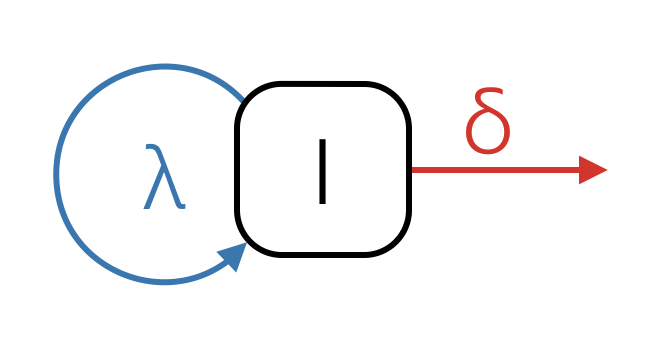
\includegraphics[width=0.250000\textwidth]{figures/bd_model.png}
    \caption{A schematic of a simple birth death model.}
    \label{fig:bd_model}
\end{figure}

In addition, the model has an origin parameter. Whereas
coalescent models work backward-in-time from the sampled sequences,
birth-death models work forward-in-time from the origin. Hence, the
model needs an origin time, which can also be jointly estimated along
with the other parameters. The origin will always be bigger than the
tMRCA of the sampled tree, since the sampled tree is by definition
smaller than the complete tree.

The \textbf{Birth Death Skyline Serial} model we used was
parameterized in terms of $ R_e $ and
$ \delta $. Recall that $ R_e > 1 $ means that
an epidemic will keep growing. We can see this from the definition of
$ R_e $ as the ratio of the birth and death rates.

\begin{equation}
    R_{e} = \frac{\lambda}{\delta}
\end{equation}

% \begin{longtable}[]{@{}rl@{}}

% if $ \lambda > \delta $ then $ R_e > 1 $ &
% epidemic grows\tabularnewline
% if $ \lambda = \delta $ then $ R_e = 1 $ &
% epidemic stays constant\tabularnewline
% if $ \lambda < \delta $ then $ R_e < 1 $ &
% epidemic declines\tabularnewline

% \end{longtable}

We used this paramerization simply because it is often easier to specify
priors for $ R_e $ than the transmission rate, and because
$ R_e $ is often more informative for prevention efforts. 

In addition, the model assumes that the data are heterochronous (sampled
at different times). It assumes that:

\begin{equation}
    \delta = \psi + \mu
\end{equation}

where $ \psi $ is the rate at which lineages are sampled
through time and $ \mu $ is the rate at which lineages are
removed from the tree for any other reason (death, recovery, extinction
etc.). (In this case the $ \rho $ parameter is no-longer
available, because samples are collected through time, and not just at
one timepoint). By default, the model is parameterized in terms of
$ R_e , \delta $ and $ p $, the sampling
proportion:

\begin{equation}
    p = \frac{\psi}{\psi + \mu}
\end{equation}

The sampling proportion is the proportion of all removed lineages that
were sampled, and can be used to obtain a rough estimate of the total
population size. This model is useful for studying infectious disease
dynamics, because samples are often collected over the course of an
epidemic. 

You can also see that the model \textbf{Birth Death Skyline Serial}
assumes that upon sampling a lineage is removed from the tree (e.g.~in a
disease model the sampled individual cannot transmit the disease after
sampling). The consequence for the phylogeny is that a sampled lineage
cannot be a direct ancestor of any other lineage in the tree. This
assumption can be relaxed, but we will not do so during this tutorial.

You may have noticed that there are many Birth-Death Skyline models
available in BEAUti. For example, the \textbf{Birth Death Skyline
Contemporary} model is used for homochronous data (all sequences sampled 
at the same time) and parameterized in terms of
$ \lambda, \delta $ and $ \rho $, whre $\rho$ is the sampling probability
at the present time. 


The Birth-Death Skyline model is very flexible and allows any or all of
these rates to change independently over time. This is done by dividing
the time from the origin to the most recent sample into dimension
$ d $ equally spaced intervals (see Figure
\ref{fig:bdsky_principle}). The rates are then allowed to change between
intervals. Since some rates (e.g. $ \lambda $ and
$ \delta $) are highly correlated, it is not always a good
idea to let all rates change over time because it can lead to poor
mixing or biased estimates. It is also possible to specify the
change-point times more flexibly, or even estimate them, however for now
this requires editing the XML file. Some examples are available
\href{https://github.com/laduplessis/skylinetools/wiki/TreeSlicer}{here}.

\begin{figure}
    \centering
    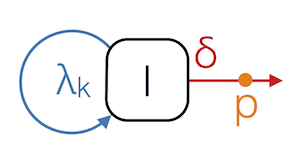
\includegraphics[width=0.250000\textwidth]{figures/bdsky_model.png}
    \caption{A schematic of the Birth Death Skyline Serial model.}
    \label{fig:bdsky_model}
\end{figure}

\begin{figure}
    \centering
    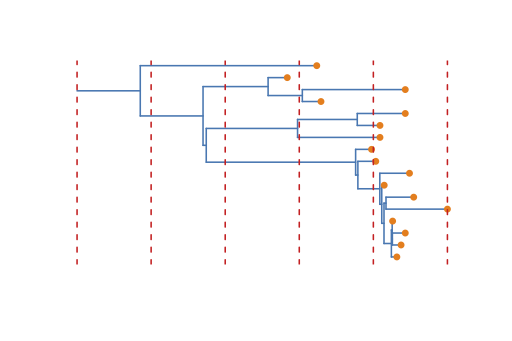
\includegraphics[width=0.750000\textwidth]{figures/bdsky_intervals5.png}
    \caption{Example tree where the red dotted lines are an example of where rates could be allowed to change on the tree. The branch at the root (compare Figure~\ref{fig:coal_events}) is indicating the origin of the epidemic, which is also estimated in the BDSKY.}
    \label{fig:bdsky_principle}
\end{figure}


\subsection{Analyzing the Coalescent Bayesian Skyline results}


Once BEAST2 has finished running the coalescent Bayesian Skyline analysis, 
open Tracer to get an overview of the BEAST2 output. When the main window has opened, choose
\lstinline!File > Import Trace File...! and select the file called
\lstinline!bsp_777.log! that BEAST2 has created, or simply drag
the file from the file manager window into Tracer.

\begin{framed}
Open \textbf{Tracer}. Drag and drop the \lstinline!bsp_777.log!
file into the open Tracer window.

Alternatively, use \textbf{File \textgreater{} Import Trace
File\ldots{}} (or press the \textbf{+} button below the \textbf{Trace
Files} panel) then locate and click on \lstinline!bsp_777.log!.
\end{framed}


\begin{figure}
    \centering
    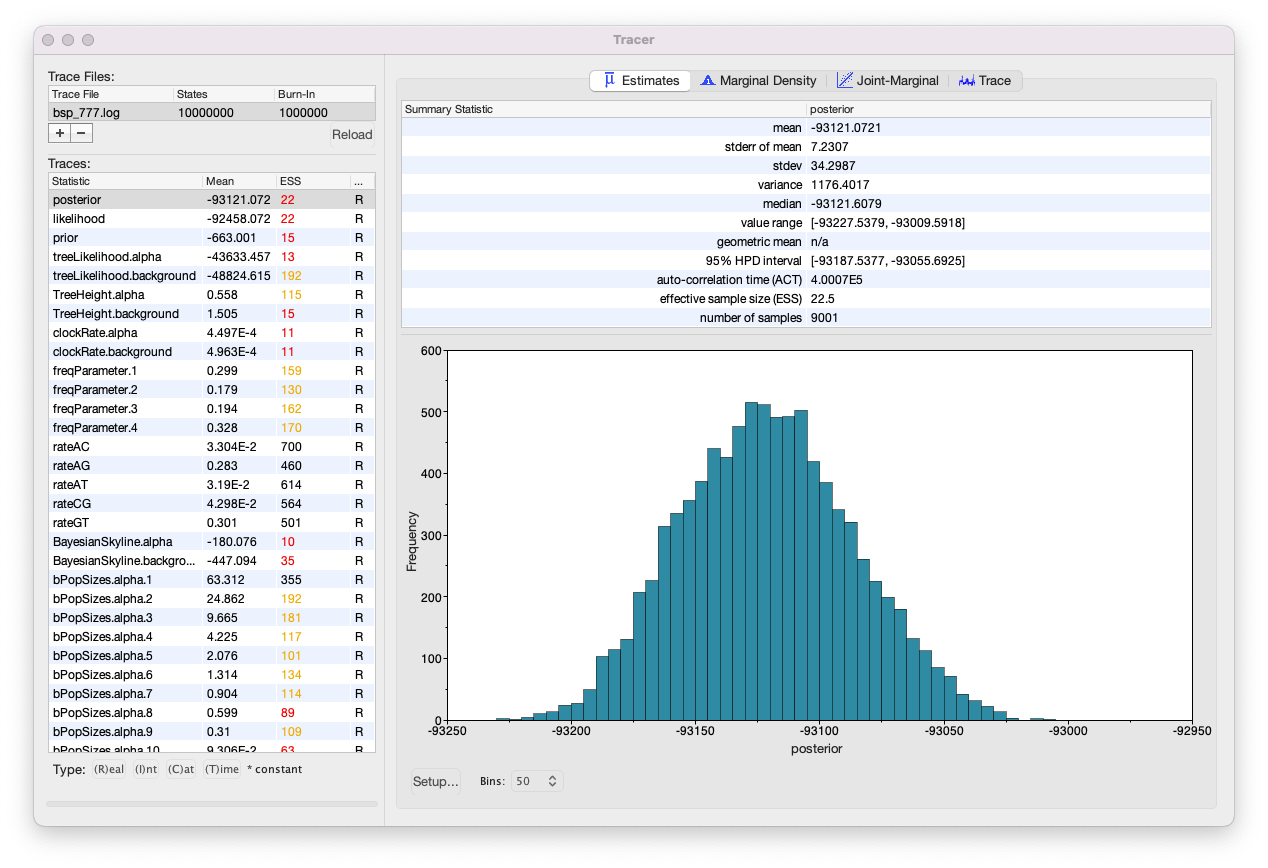
\includegraphics[max width=\textwidth, max height=0.9\textheight]{figures/tracer_bsp.png}
    \caption{Tracer showing a summary of the BEAST2 run of the coalescent Bayesian Skyline plot with an MCMC chain length of 10'000'000 and no constraints.}
    \label{fig:tracer_bsp}
\end{figure}

The Tracer window should look as shown in Figure \ref{fig:tracer_bsp}.
Because we only ran a short chain for a complicated analysis many parameters have very low ESS
values. You can find a log file of an identical analysis that was run for 100 million MCMC steps in the 
\lstinline!precooked_runs/! folder (\lstinline!bsp_long.log!).


Note that many parameters have either \lstinline!.alpha! or \lstinline!.background! appended to their
names. These are parameters that we inferred independently for the Alpha and background alignments/partitions. 
The \lstinline!popSizes! parameters represent the effective population sizes for each alignment in each interval, 
whereas the \lstinline!groupSizes! parameters are the sizes of each interval (more specifically, the 
number of coalescent events within an interval). Since populations naturally grow/decline through 
exponential growth/decay, it is more natural to visualise the population sizes on a log scale. 

\begin{framed}
  Select the \textbf{Marginal Density} tab.

  \begin{itemize}
      \item
        Select all of the \textbf{popSizes.alpha} parameters using \textbf{shift + click}.
      \item 
        Open the \textbf{Display} drop-down menu and select \textbf{Violin}.
      \item
        Click on the setup button at the bottom and check \textbf{Log axis}.
  \end{itemize}

\end{framed}

We see that the effective population size of Alpha appears to have grown linearly on a log scale, 
which translates to exponential growth. Similarly, the background appears to have first grown exponentially, 
and then stabilised at a constant population size. On the other hand, the group sizes parameters were 
not inferred very precisely and there is a large variation in their sizes (Figure~\ref{tracer_sizes}). This 
indicates smooth population size changes. 

\begin{figure}
    \centering
    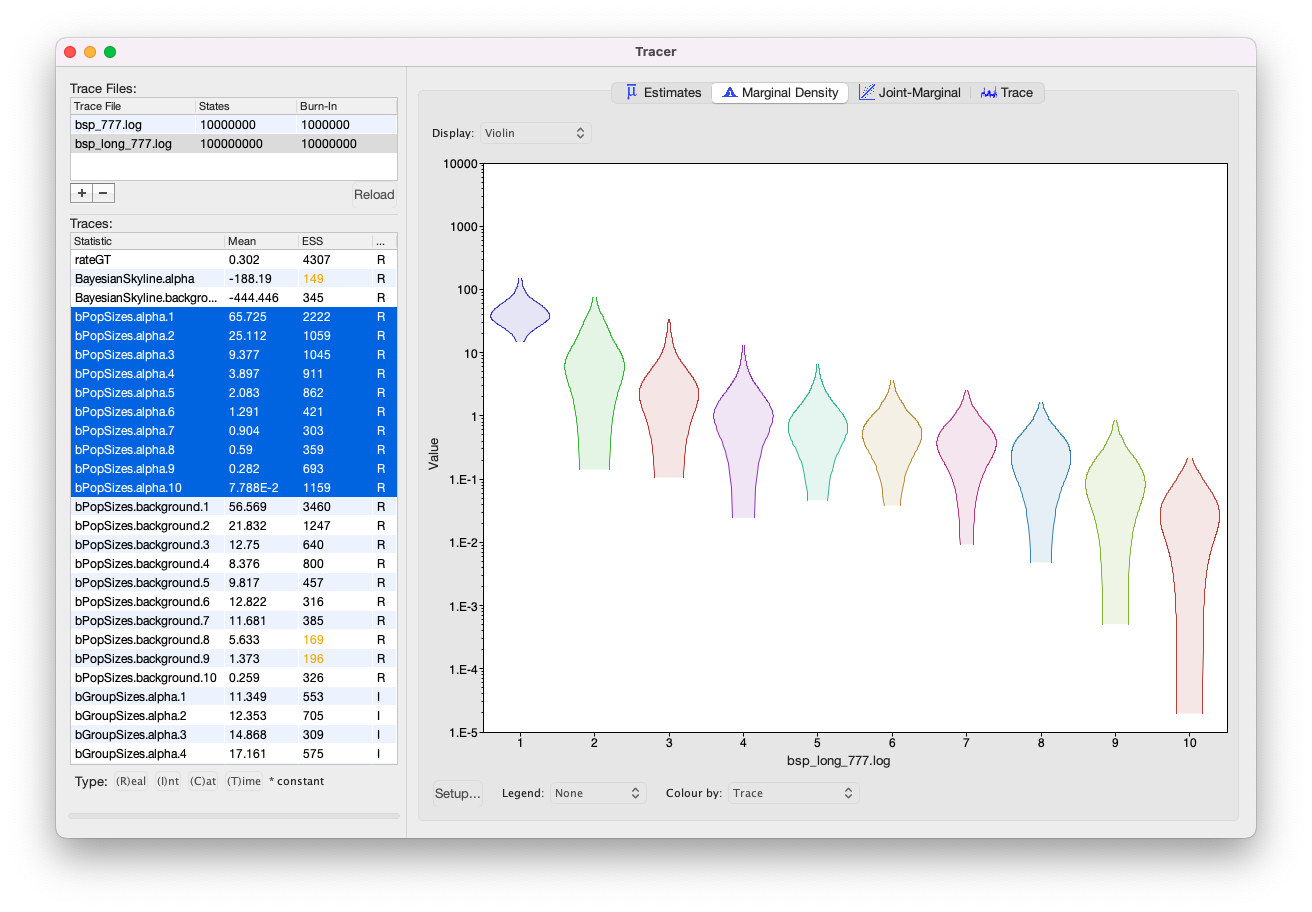
\includegraphics[max width=0.75\textwidth, max height=0.9\textheight]{figures/popSizes.png}
    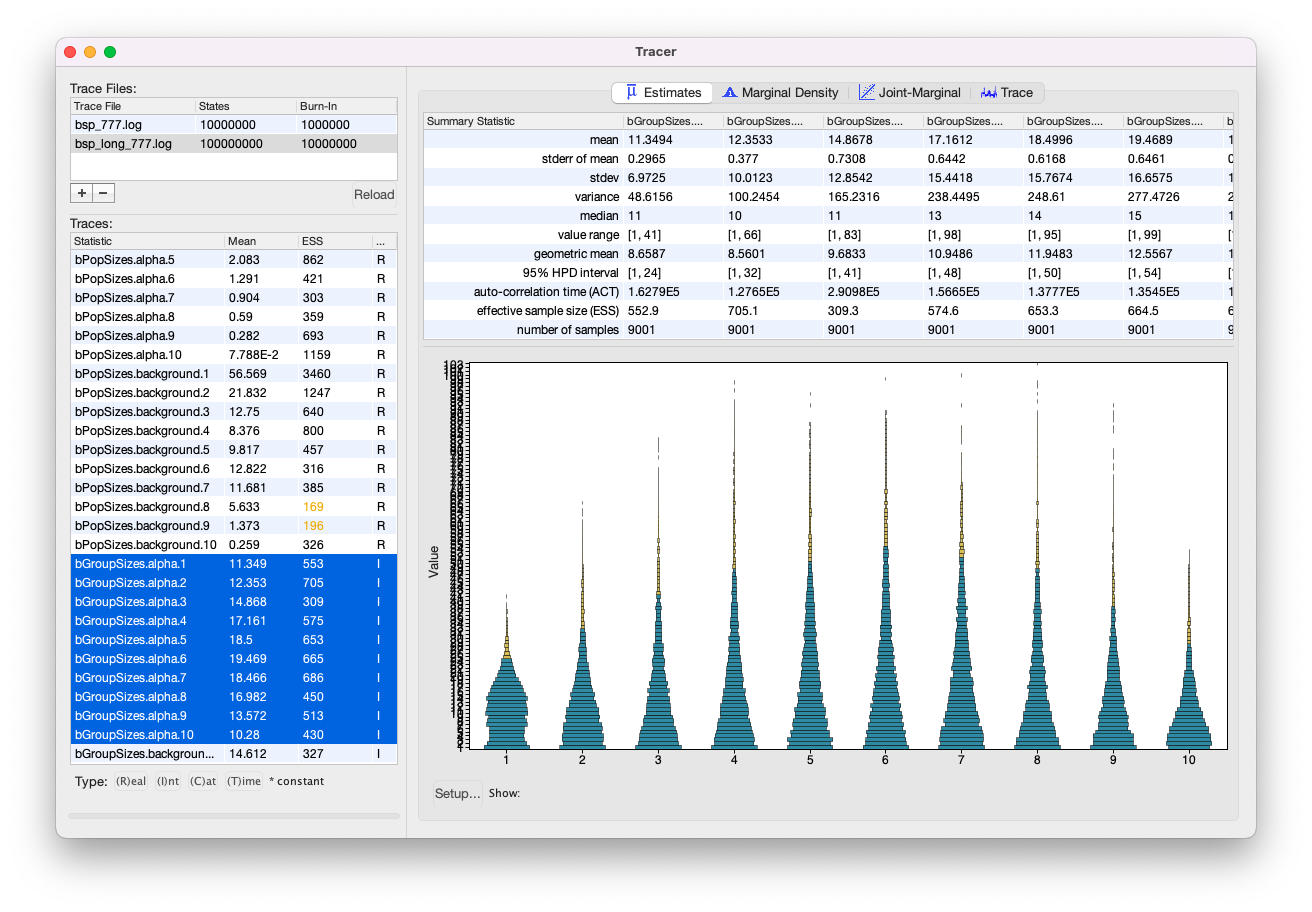
\includegraphics[max width=0.75\textwidth, max height=0.9\textheight]{figures/groupSizes.png}
    \caption{Visualising the population sizes and group sizes in Tracer.}
    \label{fig:tracer_sizes}
\end{figure}

However, these are just indications, and we need to combine both parameters to reconstruct the 
population dynamics. To do that Tracer needs to know when the coalescent events on each posterior 
tree was, and therefore also needs the \lstinline!*.trees! file. This is the reason why it's important 
to log the trace and tree files at the same frequency for the coalescent Bayesian Skyline plot. 
But before we can do that, we need to know the decimal date at the time of the most recent sample in 
our dataset (March 1st, 2021).

\begin{framed}
  Open R or Rstudio.

  Type in: 
  \begin{lstlisting}[language=R]
library(lubridate)
lubridate::decimal_date(ymd("2021-03-01"))
  \end{lstlisting}

  This should give: 
  \begin{lstlisting}[language=R]
[1] 2021.162
  \end{lstlisting}


Return to Tracer and navigate to \textbf{Analysis \textgreater{} Bayesian Skyline
Reconstruction}. 

\begin{itemize}
  \item Choose \lstinline!bsp_alpha.trees! next to \textbf{Trees Log File}.
  \item Set \textbf{Population Size} to \textbf{bPopSizes.alpha} and 
        \textbf{Group Size} to \textbf{bGroupSizes.alpha}.
  \item Set the \textbf{trace of the root height} to \textbf{TreeHeight.alpha}.
  \item Check the \textbf{Use manual range for bins} checkbox and enter 
        \textbf{2020} and \textbf{2021.162} for the minimum and maximum times.
  \item Enter \textbf{2021.162} for the \textbf{Age of youngest tip}. 
  \item Press \textbf{OK} to reconstruct the past population dynamics (Figure~\ref{fig:bsp_reconstruction}). 
\end{itemize}

Without closing the resulting plot, go back to the main Tracer window and 
repeat the same steps for the background alignment. 

\end{framed}

\begin{figure}
    \centering
    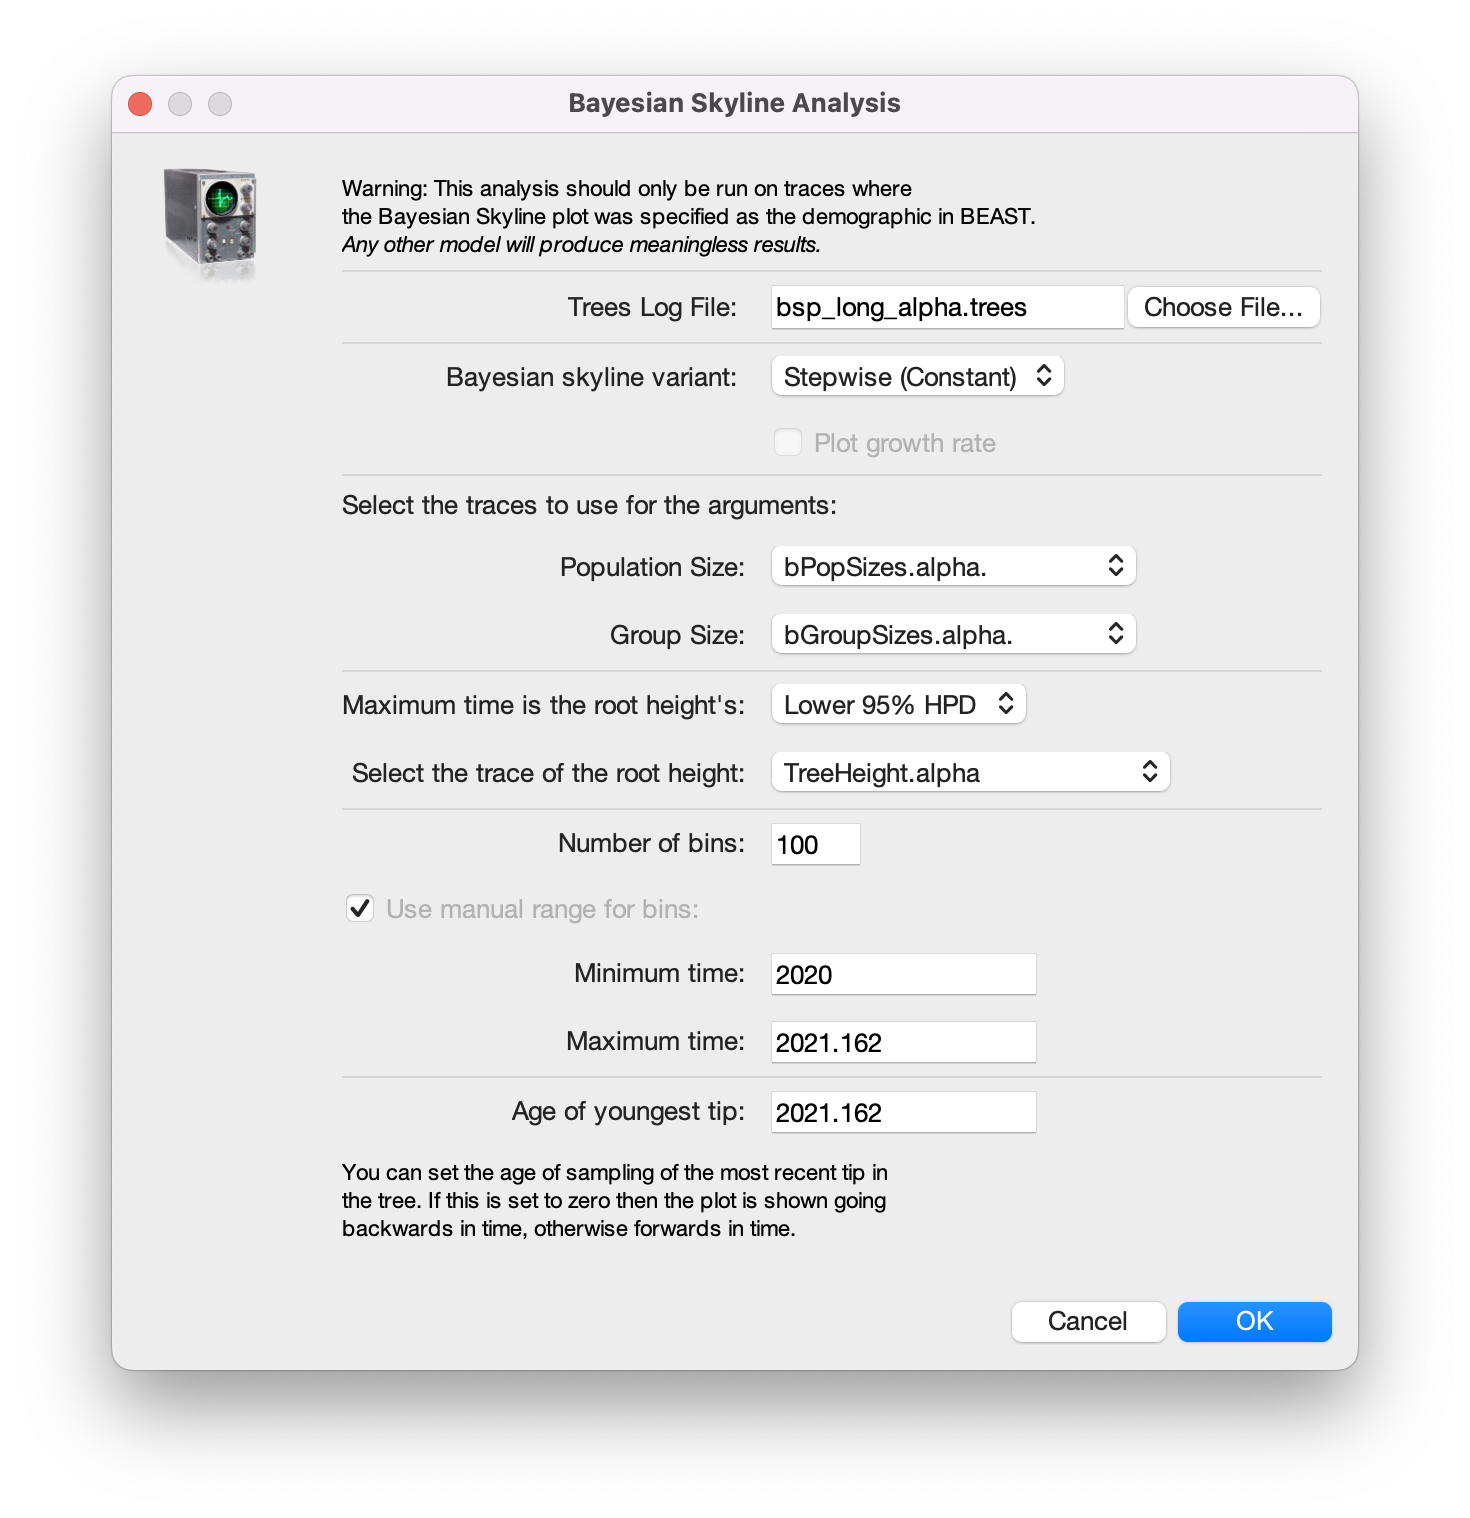
\includegraphics[width=0.750000\textwidth]{figures/bsp_reconstruction.png}
    \caption{Reconstructing the Bayesian Skyline plot in Tracer.}
    \label{fig:bsp_reconstruction}
\end{figure}

\begin{figure}
    \centering
    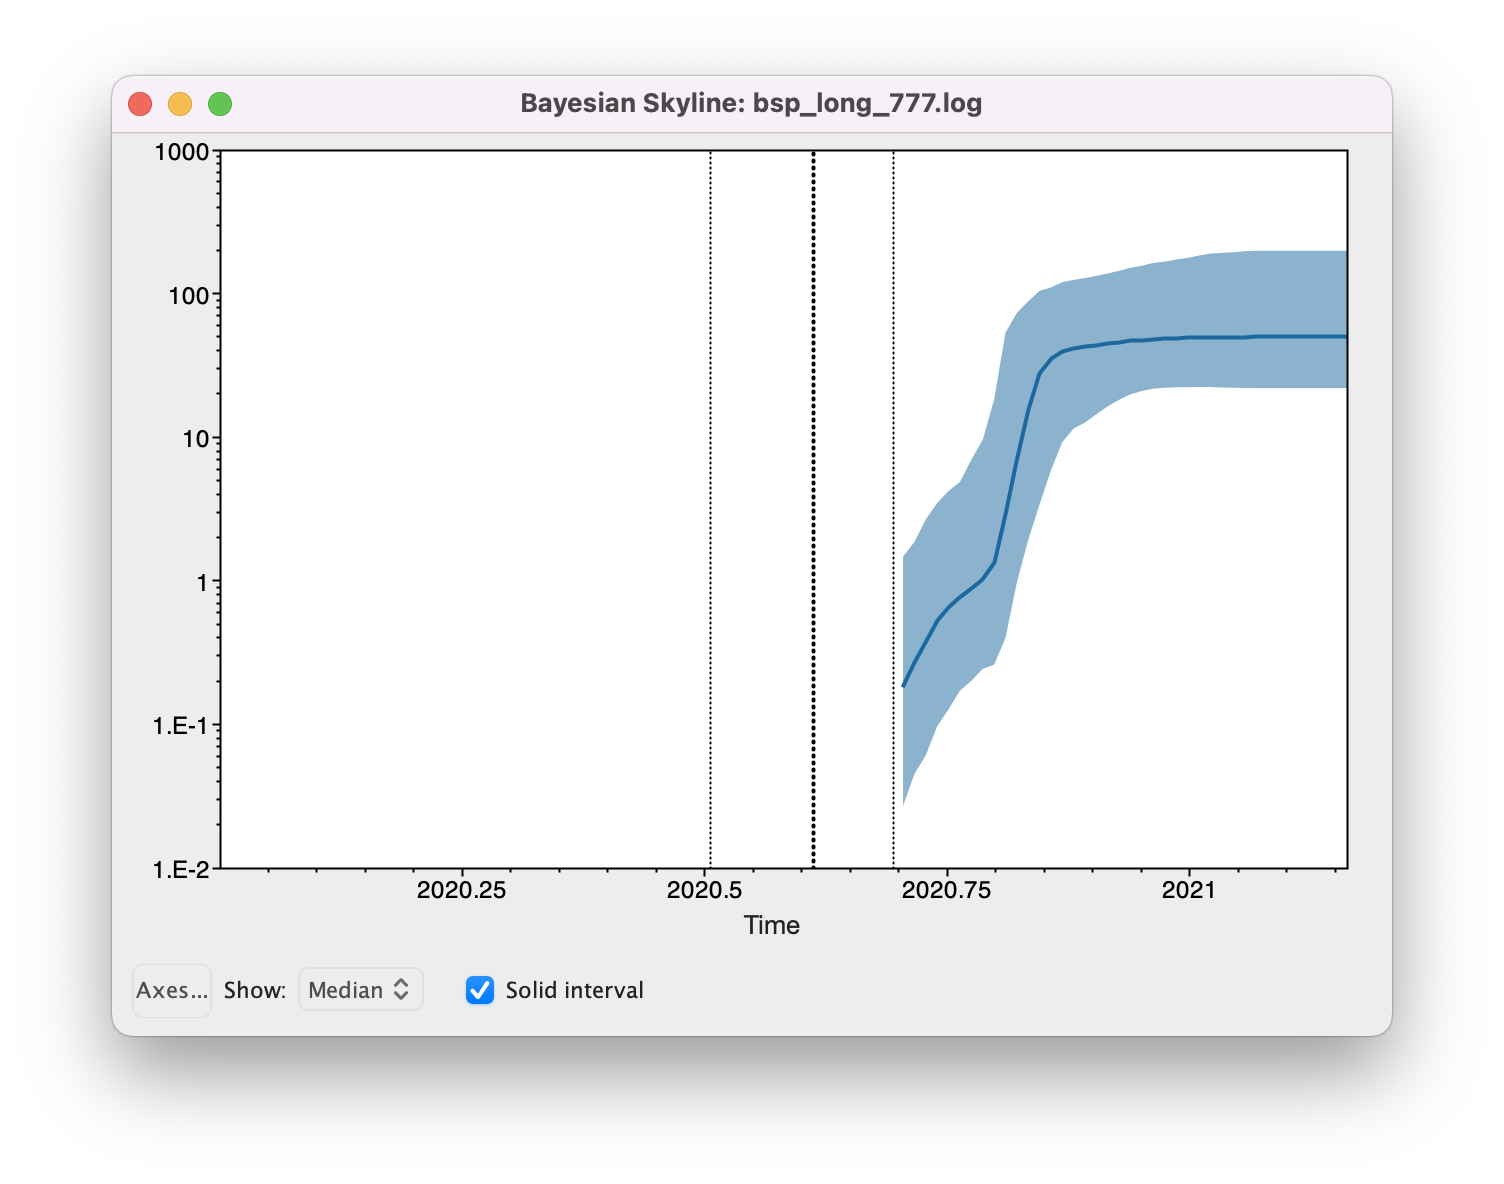
\includegraphics[width=0.75\textwidth]{figures/bsp_alpha.png}
    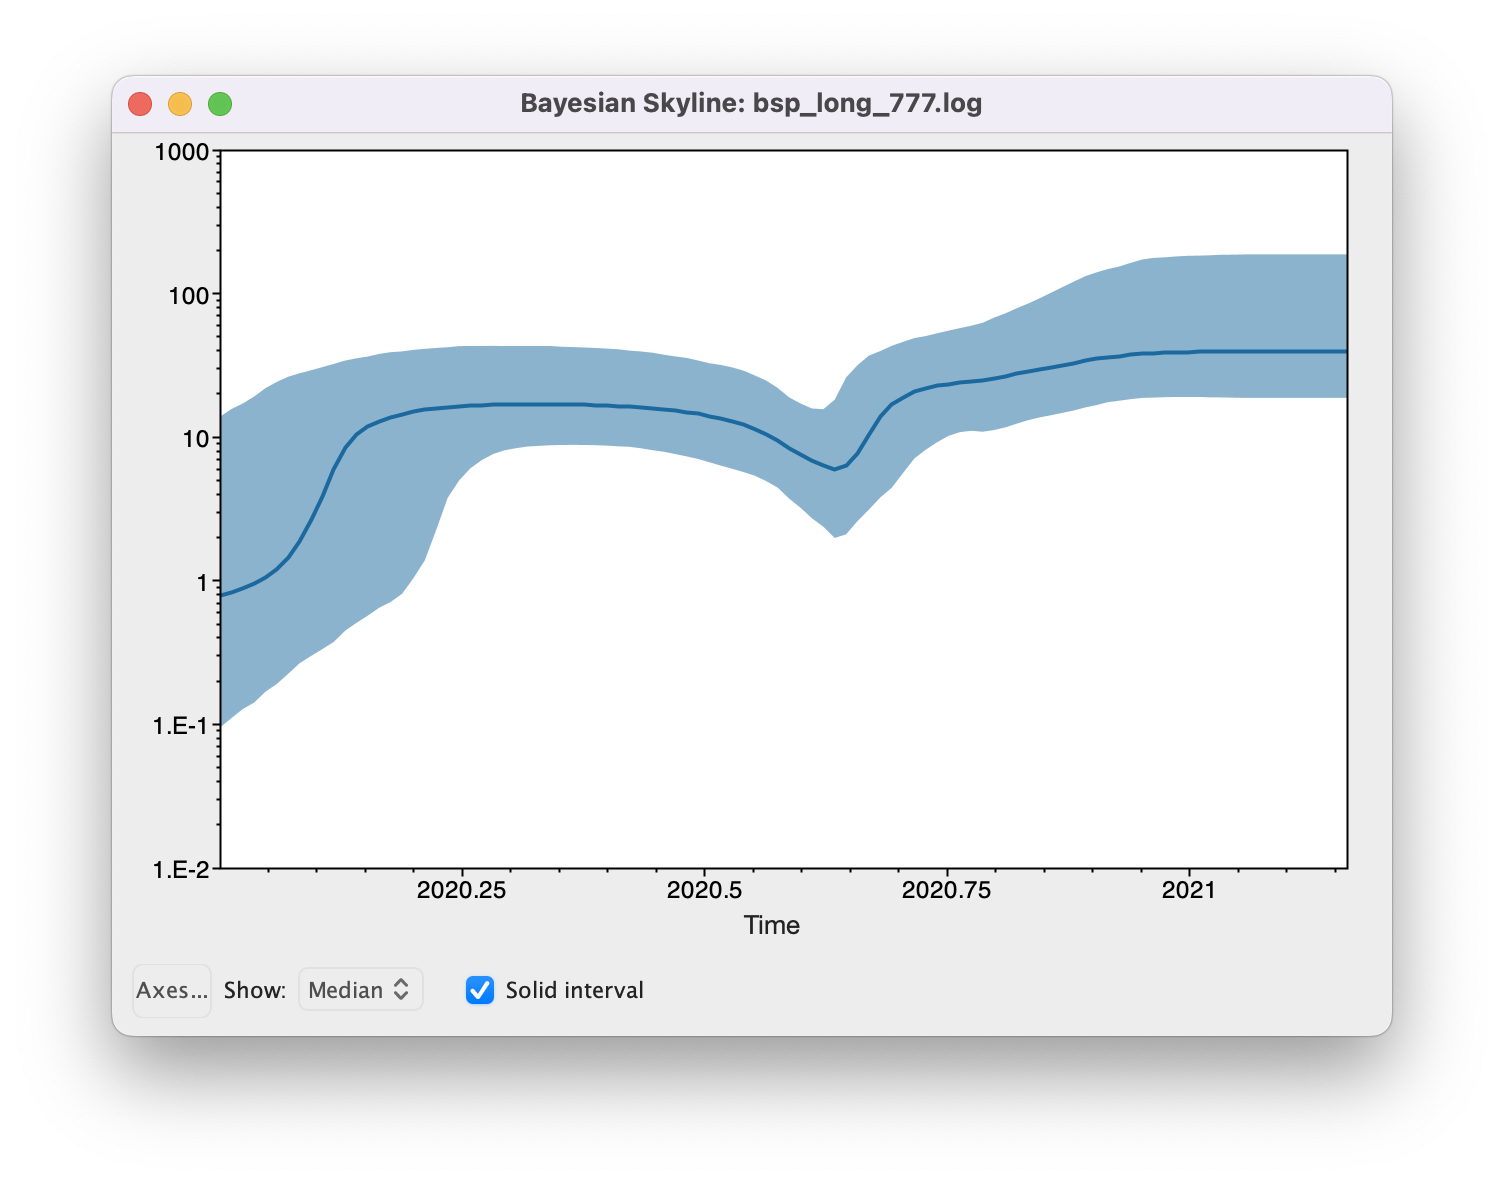
\includegraphics[width=0.75\textwidth]{figures/bsp_background.png}
    \caption{Coalescent Bayesian Skyline analysis output. The thick line is the median estimate of the estimated effective population size (can be changed to the mean estimate). The solid interval
    represents the upper and lower bounds of the 95\% HPD interval. The x-axis is the time in years and the y-axis is on a log-scale.}
    \label{fig:bsp_traces}
\end{figure}



This should reconstruct the population dynamics for both alignments across the same time period
(Figure~\ref{fig:bsp_traces}). In general it is not necessary to use a manual range for the bins, 
but we used it here to ensure that both plots are over the same X-axis range and more easily 
comparable. There are two ways to save the analysis, it can either be saved as a
\lstinline!*.pdf! for display purposes or as a tab delimited file, which can be loaded in R 
and used for custom plots (Figure~\ref{fig:bsp_combined}).

\begin{framed}
Navigate to \textbf{File \textgreater{} Export Data Table}.

Enter the filename as \lstinline!hcv_coal.tsv! and save the file.
\end{framed}

\begin{figure}
    \centering
    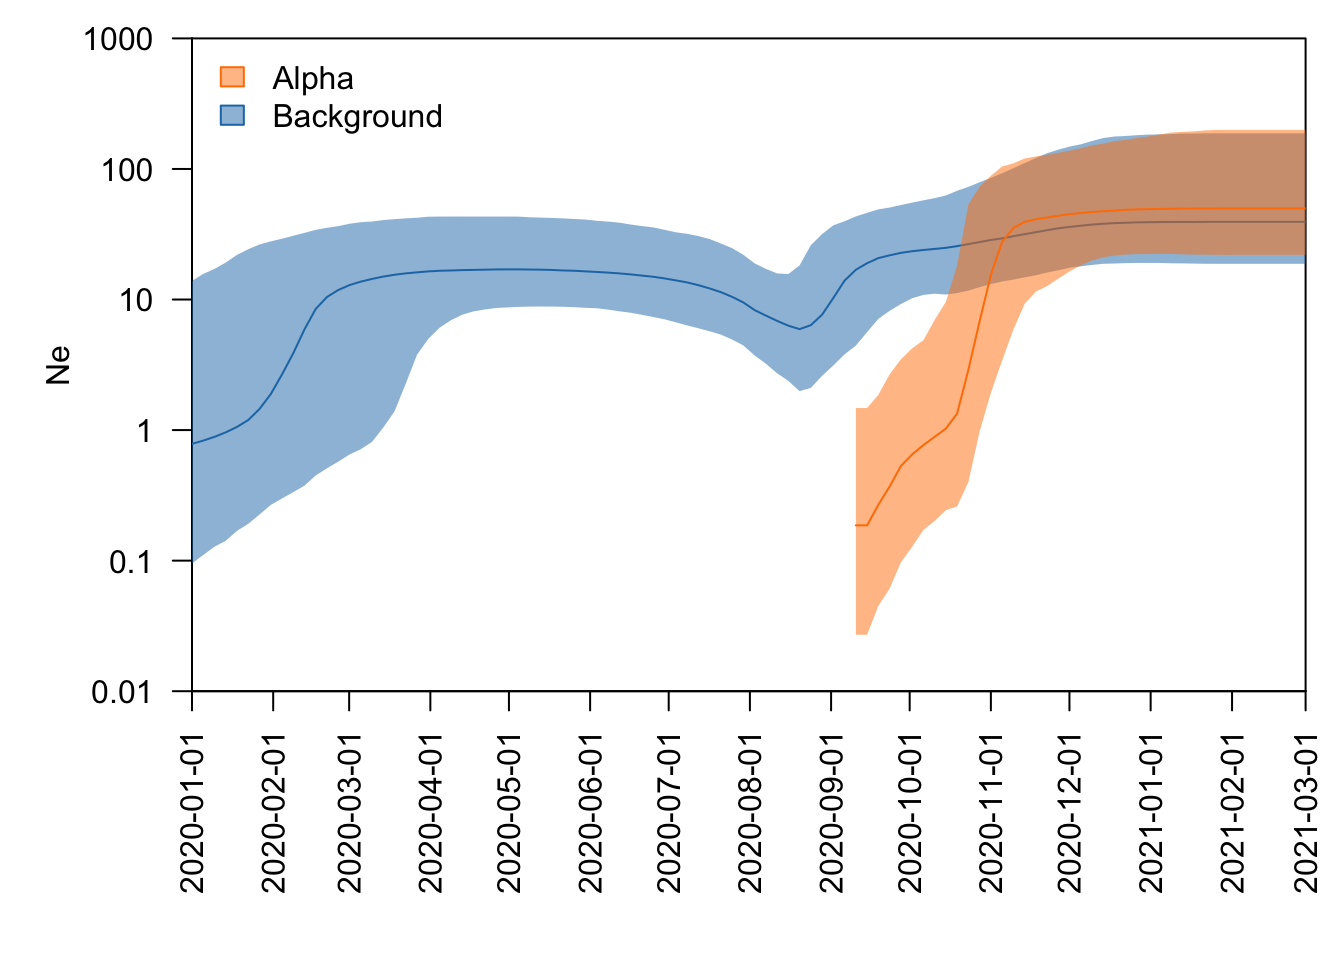
\includegraphics[width=0.750000\textwidth]{figures/bsp_combined.png}
    \caption{Both Bayesian Skyline Plots on one set of axes.}
    \label{fig:bsp_combined}
\end{figure}





\subsection{Analyzing the Birth Death Skyline results (i)}

If we open the trace file for the Birth Death Skyline analysis we notice that the ESS values are even 
lower. The trace for the origin of the Alpha alignment is especially bad and 
highly autocorrelated (Figure~\ref{fig:tracer_origin}). Recall that the samples in the trace should approximate 
uncorrelated draws from the target distribution, which should result in the traces resembling white noise.
Obviously we would have to run this analysis much, much, much longer for this parameter to begin mixing well. 
Even looking at the results from an analysis that was run for 100 million steps, the parameter still has an 
ESS below 100. Another concern is the origin of the background alignment. Although it mixes well, it is 
estimated to be greater than 5 years! The implication would be that the index case of SARS-CoV-2 existed 
some time in 2015! This seems counter to everything we know about the pandemic. Not even the most outrageous 
conspiracy theories hypothesize that the virus already circulated in 2015. 
Even if we choose to believe these results, this 
analysis wouldn't tell us much about the population dynamics of the background dataset during the 
COVID-19 pandemic. Because the period from the origin to the most recent sample is divided into 10 
equidistant intervals, all of the dynamics during the pandemic are encapsulated within the last 3 intervals 
and all other intervals simply recover the prior expectation we set on $R_e$. 

\begin{figure}
    \centering
    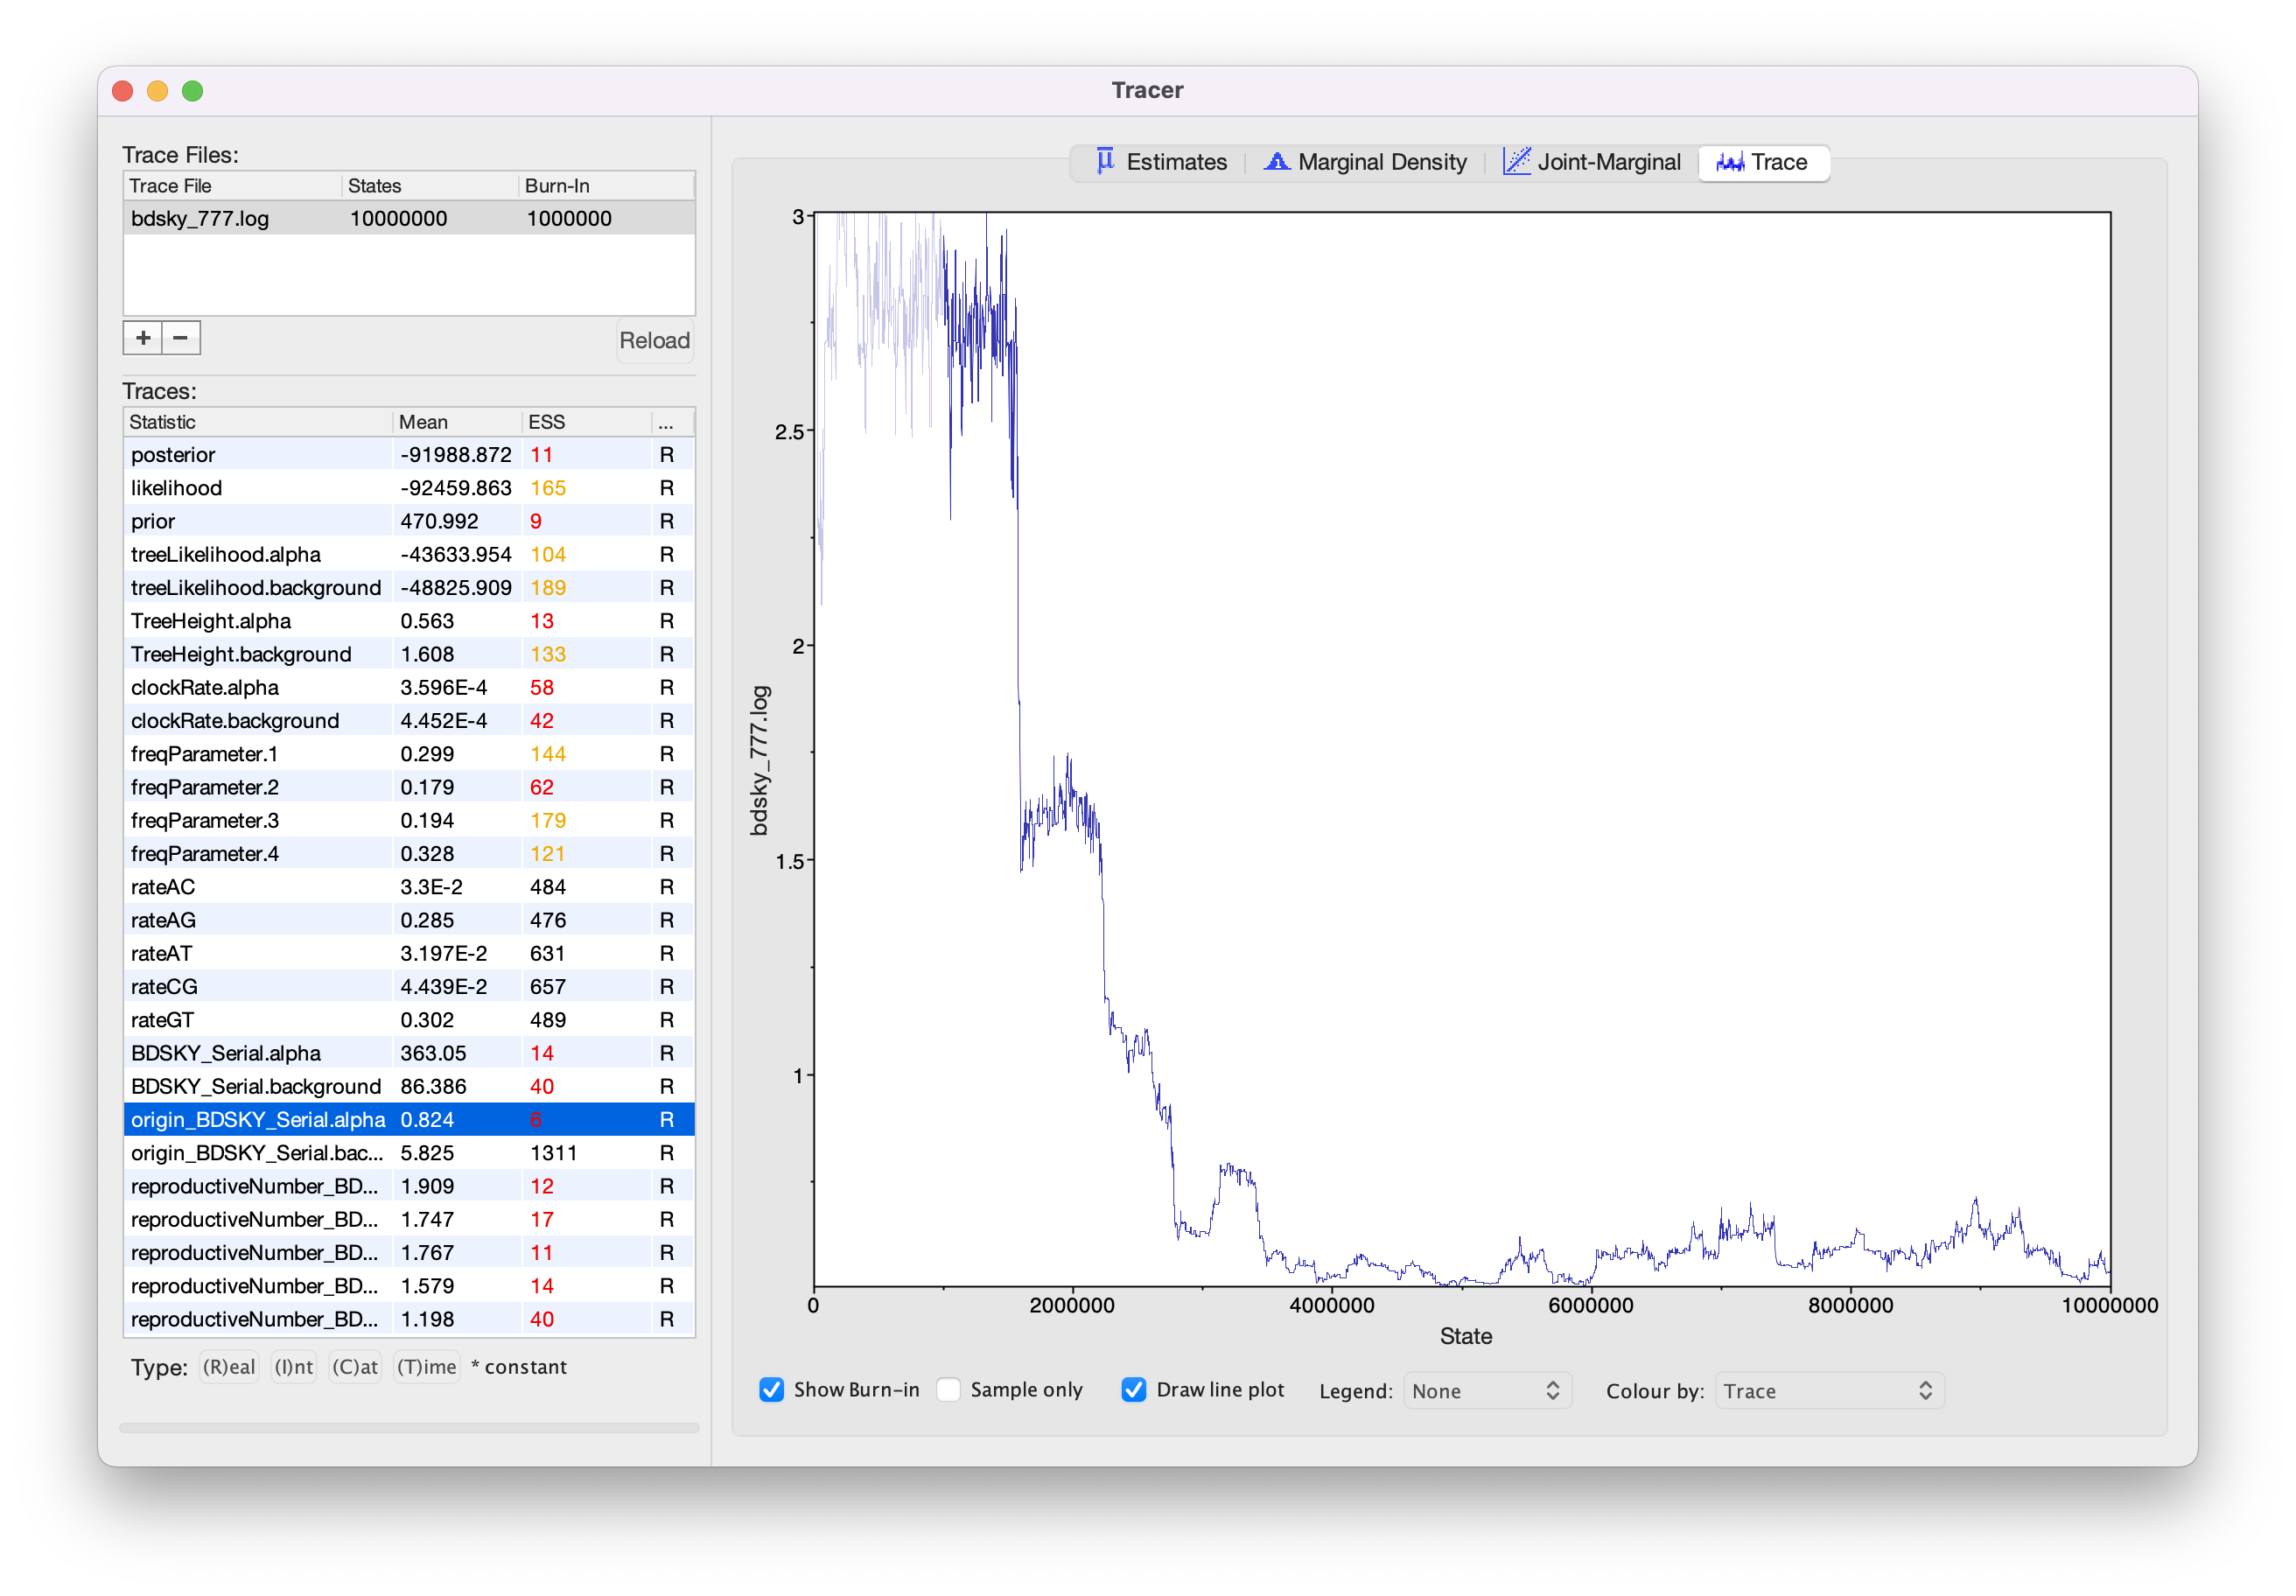
\includegraphics[max width=\textwidth, max height=0.9\textheight]{figures/tracer_origin.png}
    \caption{Trace of the origin of the Alpha alignment after 10'000'000 MCMC steps.}
    \label{fig:tracer_origin}
\end{figure}


\subsection{Conditioning the Birth Death Skyline on the root}

  The Birth Death Skyline model occasionally has difficulty inferring the time of the origin of an epidemic. 
  This parameter represents the index case and may have existed long before the oldest sample 
  in the dataset was collected and sometimes also long before the tMRCA of all sequences in the 
  dataset. If the epidemic has a constant growth rate over time it is straighforward to infer the 
  time of the origin. However, the Birth Death Skyline explicitly allows the growth rate to change 
  over time in a nonparametric fashion. 
  The end result is that there may not be enough information in the dataset to infer both changes in 
  the growth rate over time as well as the time of the origin. We can circumvent this limitation by 
  eliminating the origin parameter and ``conditioning on the root.'' In this alternative parameterisation 
  of the Birth Death Skyline model, the model is parameterised to start not at the index case, but at the time 
  when there are already two 
  lineages in the sampled tree, i.e. the tMRCA of the tree. In this case, the intervals are spaced
  equidistantly between the tMRCA and the most recent sample. 

  \begin{framed}
    Select the \textbf{Priors} tab.

    Select \textbf{Birth Death Skyline Serial Cond Root} in the drop-down menus next to \textbf{Tree.t:alpha} and 
    \textbf{Tree.t:background}.

    Now repeat the steps for the \textbf{Birth Death Skyline Serial} model to set the reproductive number 
    and sampling proportion priors, change the dimension of the sampling proportions and fix the become 
    uninfectious rates (with this model there is no origin parameters and therefore no origin priors). 
  \end{framed}

  Now save the file as \lstinline!bdsky_condOnRoot.xml! and run it in BEAST2. 



\subsection{Sampling from the prior}

  It is always a good idea to sample from the prior. Ideally this should be done before running the 
  analysis, as sampling from the prior can point out issues with the model. In particular, it allows 
  us to see how much information is encoded in the priors and model structure. For example, suppose 
  our aim is to decide if non-pharmeceutical interventions (NPIs) were effective by looking at whether 
  $R_e$ dropped below one after they were implemented. If the model is constrained such that $R_e$ is 
  always below one after that time, the model is worthless for answering our question. We can't simply 
  look at the prior distributions we set in BEAUti to reach such insights, because priors often interact
  with each other in complex ways \cite{Heled2011}. The result is that the induced prior of the complete model
  may not be the same as the priors we set in BEAUti. 

  \begin{framed}
    Select the \textbf{MCMC} tab.

    \begin{itemize}
      \item Set the \textbf{Chain Length} to \textbf{50'000'000}.
      \item Expand the \textbf{tracelog} options and set the 
            \textbf{Log Every} parameter to \textbf{5000}.
      \item Expand the \textbf{treelog.t:alpha} options and set the 
            \textbf{Log Every} parameter to \textbf{5000}.
      \item Expand the \textbf{treelog.t:alpha} options and set the 
            \textbf{Log Every} parameter to \textbf{5000}.
      \item Check the \textbf{Sample From Prior} checkbox at the bottom of the window 
            (Figure~\ref{fig:sampleFromPrior}.
  \end{itemize}

  \end{framed}

  \begin{figure}
      \centering
      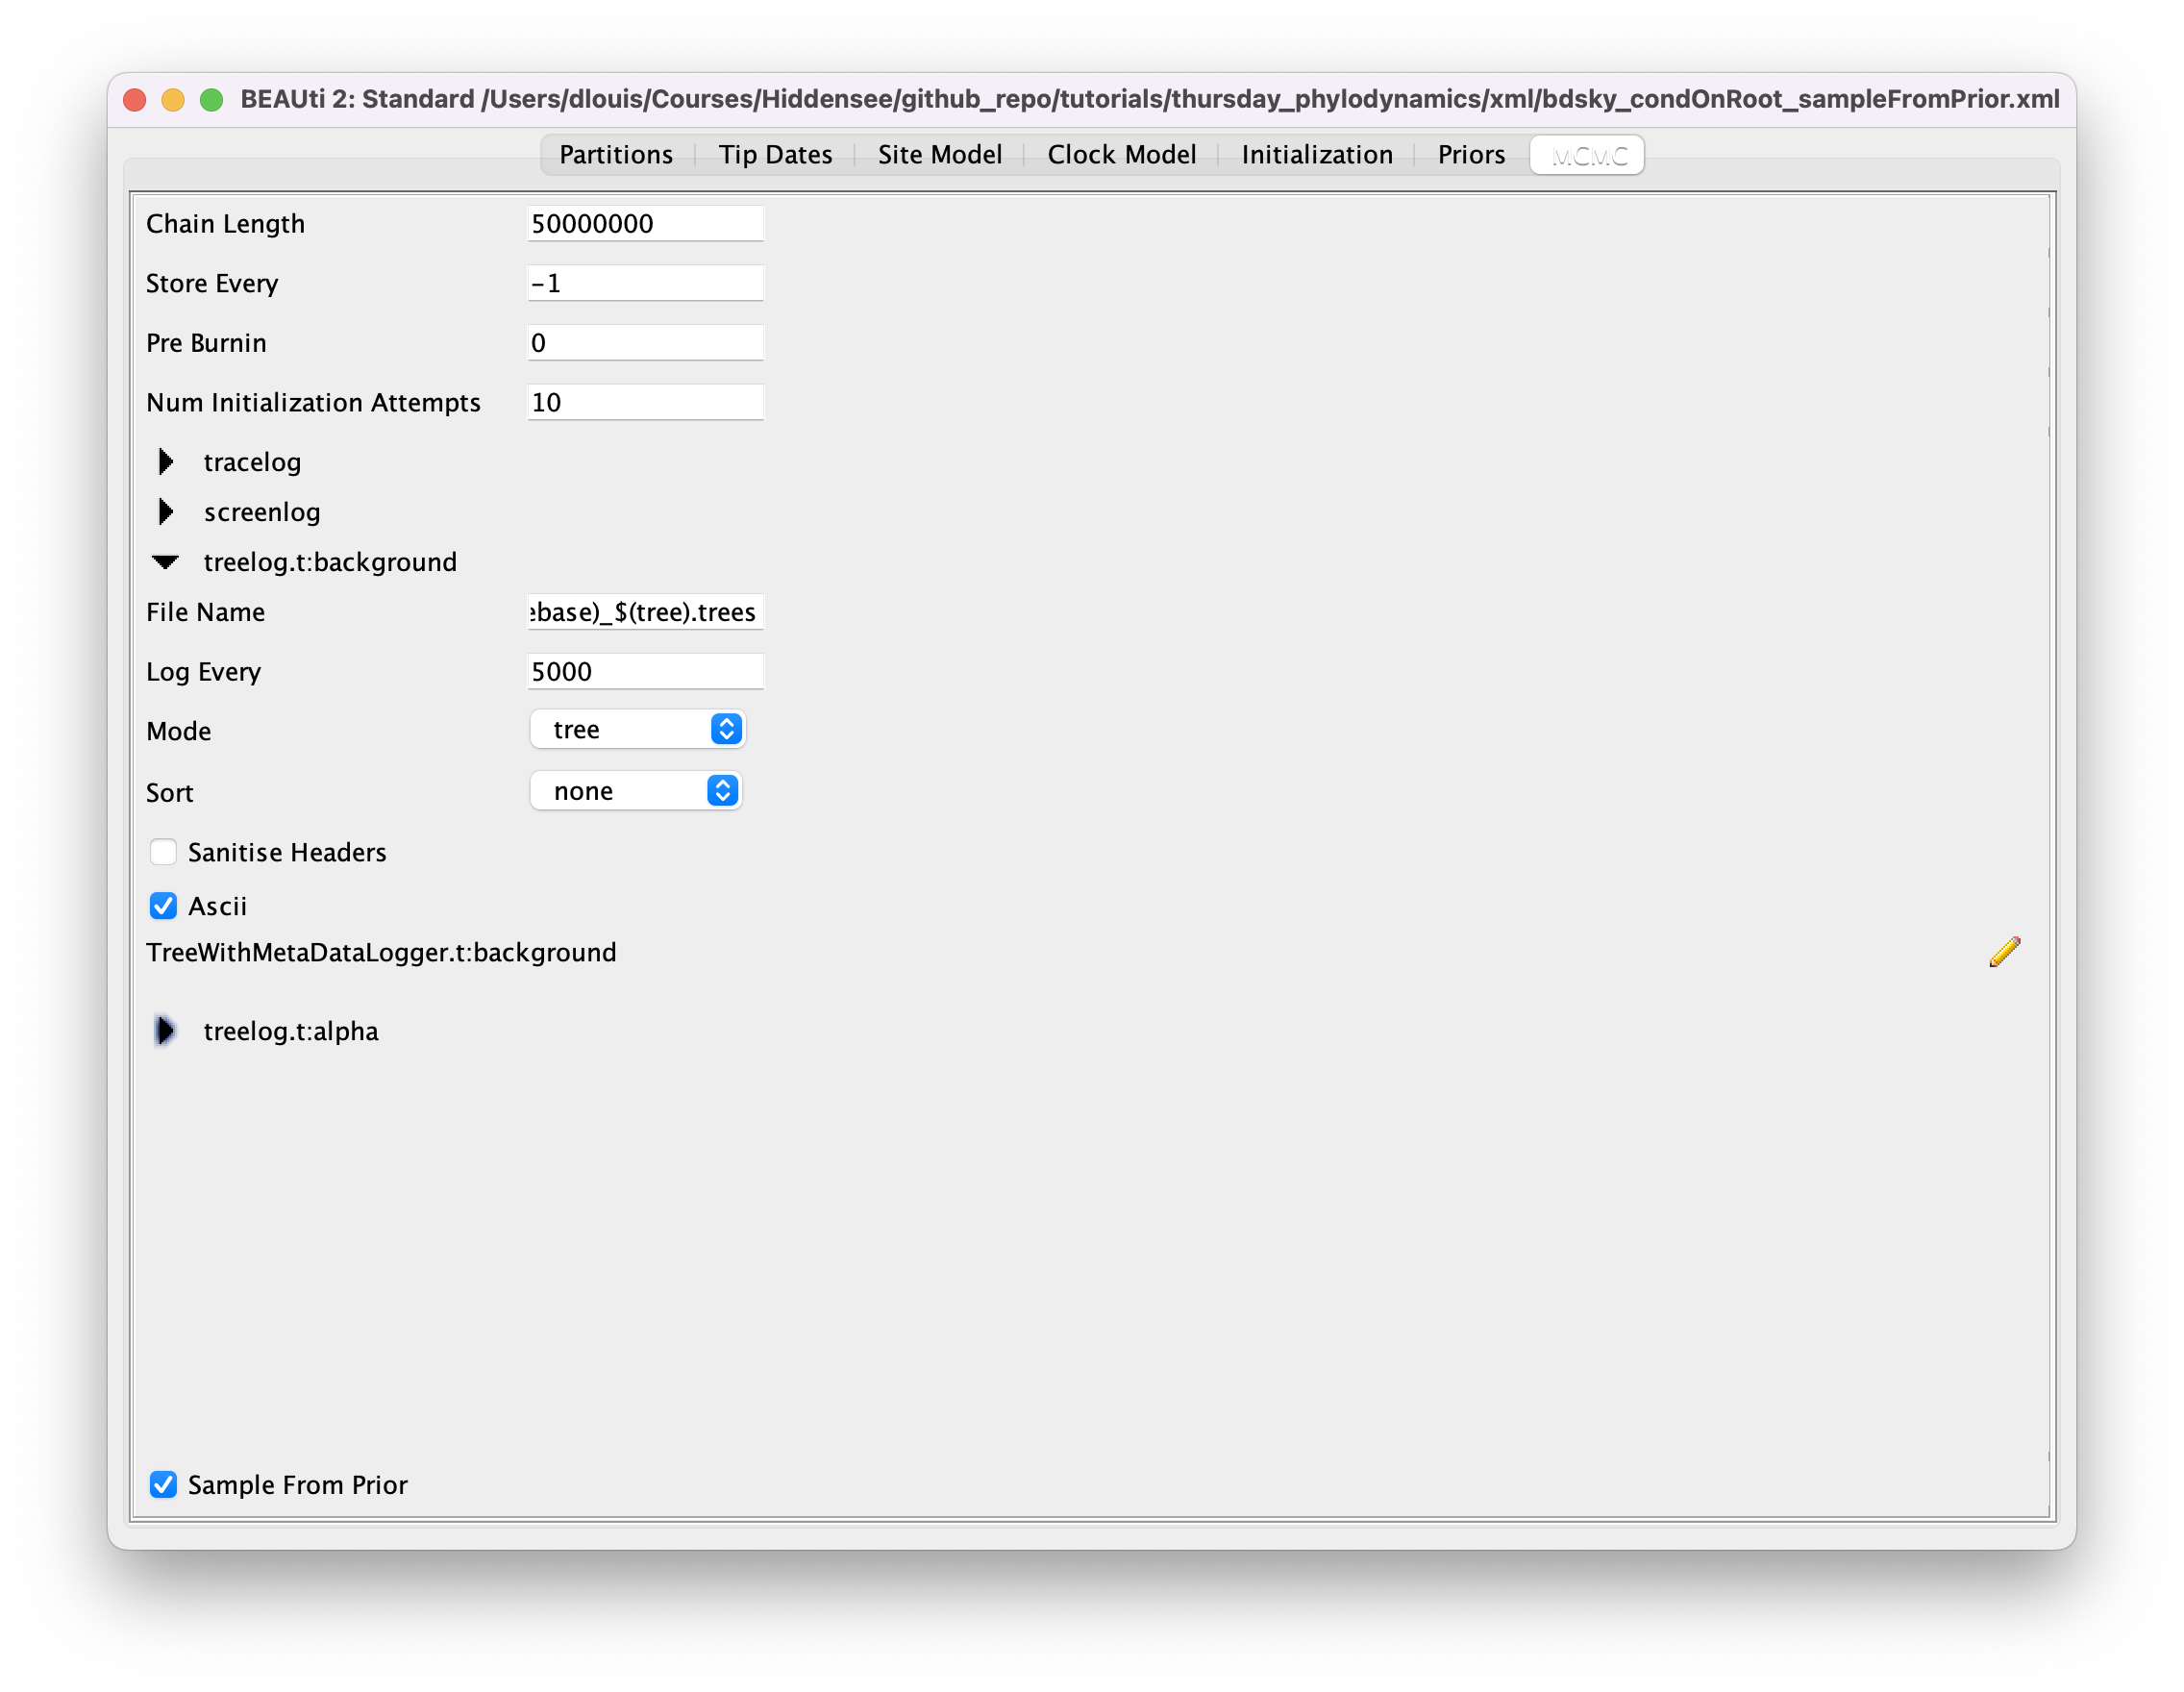
\includegraphics[max width=\textwidth, max height=0.9\textheight]{figures/sampleFromPrior.png}
      \caption{Sampling from the prior.}
      \label{fig:sampleFromPrior}
  \end{figure}

  Now save the file as \lstinline!bdsky_condOnRoot_sampleFromPrior.xml! and run it in BEAST2.

  Sampling from the prior runs the analysis without using the data. In BEAST2 this means simply masking 
  the alignment and not calculating the tree likelihood. Since calculating the tree likelihood is usually 
  the most time-consuming part of any analysis, sampling from the prior is usually much faster than 
  running the analysis. However, since there is no data, it also often has difficulty mixing and needs to be 
  run for longer. 

  Note that in the case of a heterochronous dataset, as 
  we have here, sampling from the prior still uses the sampling (tip) dates in the analysis. Strictly 
  speaking, these can also be considered part of the data. However, in our case we are also interested in 
  seeing precisely how much information the sequences are adding on top of the collection dates.


\clearpage

\subsection{Analyzing the Birth Death Skyline results (ii)}

  The trace file of the Birth Death Skyline analysis conditioning on the root
  should have better ESS values than before, although we still wouldn't expect it
  to mix well after only 10 million steps. 

  \begin{framed}
  Open \textbf{Tracer}. Drag and drop \lstinline!bdsky_condOnRoot_777.log! and 
  \lstinline!bdsky_condOnRoot_sampleFromPrior_777.log! into the open Tracer window.
  \end{framed}

\subsubsection{Visualising the Birth Death Skyline}

  There is no equivalent visualization of the skyline plot of a
  Birth-Death Skyline (BDSKY) analysis in Tracer as there is for the
  Coalescent Bayesian Skyline. But because BDSKY separates the full tree
  into equally spaced intervals, we can already get an idea of the
  inference just by looking at the inferred $ R_e $ values
  (see Figure \ref{fig:bdsky_dynamics}). This gives us a good idea of the
  trend, but it is not completely accurate. Since we are also estimating
  the tMRCA, the interval times are slightly different in each
  posterior sample and overlap slightly. The advantage of this is that we
  get a smooth estimate through time. The disadvantage is that we need to
  do some extra post-processing to plot the smooth skyline. We will use R to 
  post-process and plot the Birth Death Skyline. The below
  steps are also in an RMarkDown notebook in the \lstinline!scripts/! directory.

\begin{figure}
    \centering
    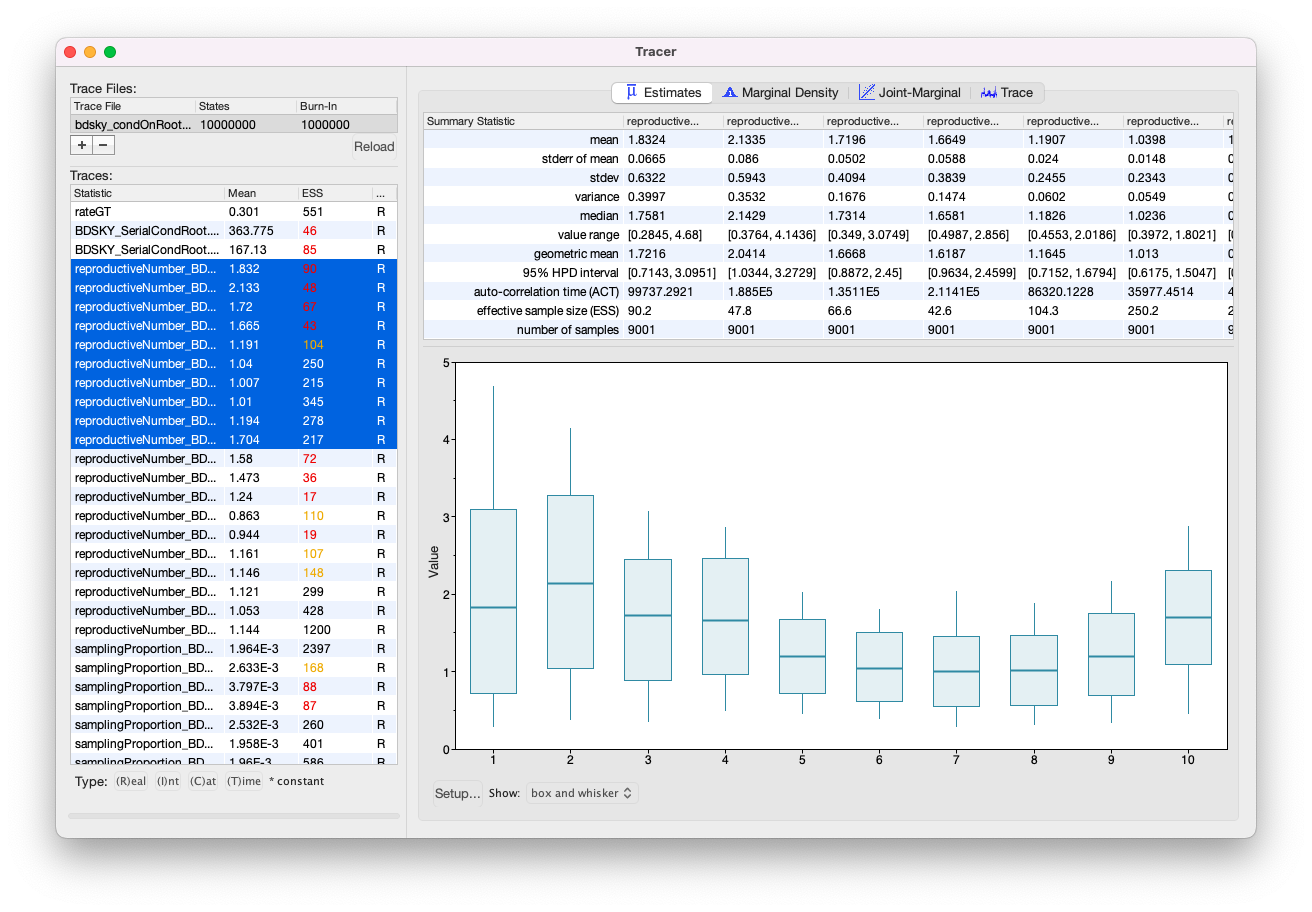
\includegraphics[max width=\textwidth, max height=0.9\textheight]{figures/bdsky_tracer.png}
    \caption{Estimated population dynamics by BDSKY in Tracer.}
    \label{fig:tracer_prior_post}
\end{figure}

  First, install
  the necessary packages. Once installed, we don't need to install the packages
  again.

  \begin{lstlisting}[language=R]
install.packages("devtools")
install.packages("lubridate")
install.packages("coda")
install.packages("RColorBrewer")
devtools::install_github("laduplessis/bdskytools")
devtools::install_github("laduplessis/beastio")
  \end{lstlisting}


  Once installed, we have to load the packages into our R workspace
  before we can use the functions in the packages. 

  \begin{lstlisting}[language=R]
library(lubridate)
library(coda)
library(bdskytools)
library(beastio)
library(RColorBrewer)
  \end{lstlisting}

  To plot the results, we need to first tell R where to find the \lstinline!*.log! 
  file of our run and then load it into R (discarding 10\% of samples as burn-in). 
  If you are using RStudio, you can change the working directory to the directory
  where you stored your log files, which makes it easier to load the files
  in R.

  \begin{lstlisting}[language=R]
bdsky_trace   <- beastio::readLog(bdsky_condOnRoot_777.log, burnin=0.1)
  \end{lstlisting}

With the trace loaded as an \lstinline!mcmc! object from the coda package we can use  
coda functions to investigate the trace and check convergence (Figure~\ref{fig:bdsky_ess}).

\begin{figure}
    \centering
    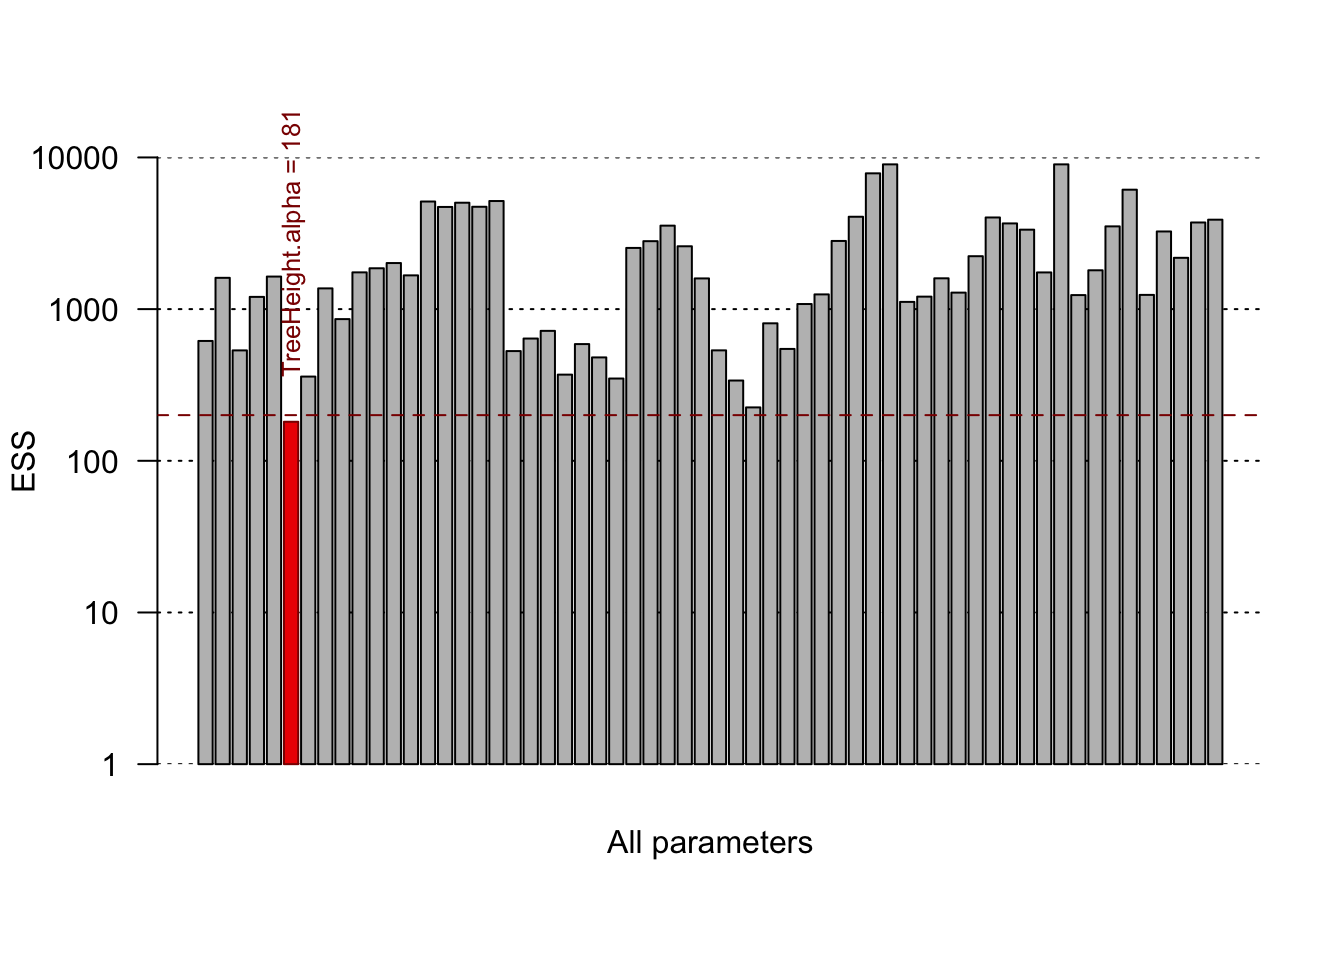
\includegraphics[width=0.600000\textwidth]{figures/plot-ESS-1.png}
    \caption{The ESS values of the trace.}
    \label{fig:bdsky_ess}
\end{figure}

Next we can extract the $R_e$ parameter values for the Alpha alignment and 
their HPDs. 

\begin{lstlisting}[language=R]
Re_alpha <- beastio::getLogFileSubset(bdsky_trace, "reproductiveNumber_BDSKY_SerialCondRoot.alpha")
Re_alpha_hpd <- t(beastio::getHPDMedian(Re_alpha))
\end{lstlisting}


We can plot the raw $R_e$ HPD intervals. This is
equivalent to the output in Tracer (Figure~\ref{fig:bdsky_hpds}).

\begin{lstlisting}[language=R]
plotSkyline(1:10, Re_alpha_hpd, type='step', ylab="R")
\end{lstlisting}

\begin{figure}
    \centering
    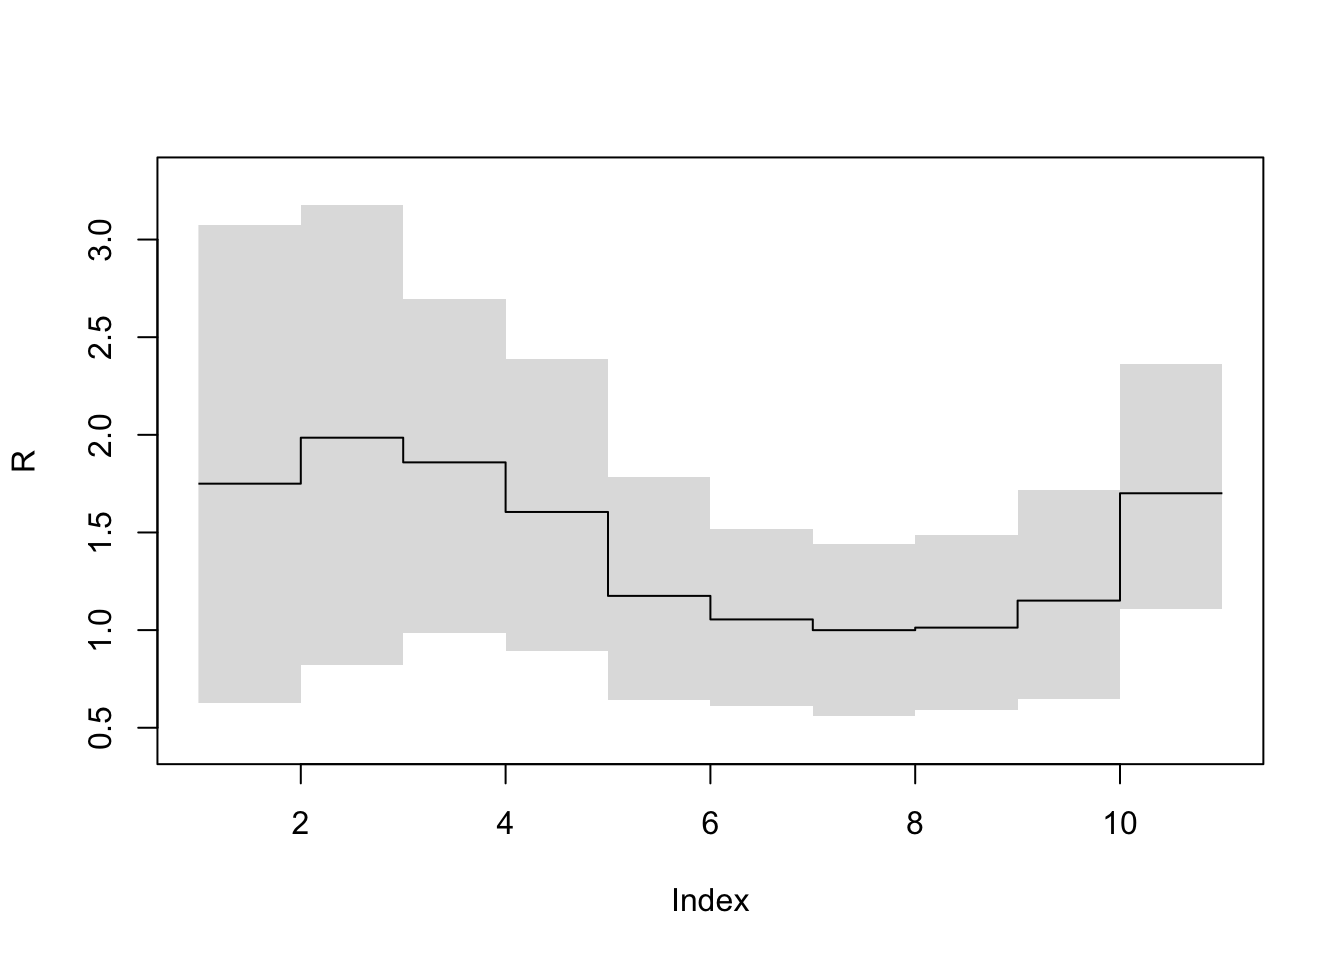
\includegraphics[width=0.600000\textwidth]{figures/bdsky_hpds.png}
    \caption{The HPDs of `$ R_e $` (equivalent to the previous figure from Tracer).}
    \label{fig:bdsky_hpds}
\end{figure}

In order to plot the smooth skyline we have to marginalise our
$R_e$ estimates on a regular timegrid and calculate the
HPD at each gridpoint. It is usually a good idea to use a grid with more
cells than the dimension of $R_e$. To do this we first
calculate the marginal posterior at every time of interest using the
function \lstinline!gridSkyline()! and then calculate the HPD for each of
the finer time intervals. The times to grid the skyline on
(\lstinline!gridTimes_alpha!), refers to years in the past. Since we conditioned 
on the root we have to use the tMRCA (\textbf{TreeHeight}) as an anchor point. 
If we didn't condition on the root we would have to use the \textbf{origin} parameter.

\begin{lstlisting}[language=R]
tmrca_alpha      <- bdsky_trace[, "TreeHeight.alpha"]
gridTimes_alpha  <- seq(0, median(tmrca_alpha), length.out=params$gridsize)  

Re_alpha_gridded <- mcmc(bdskytools::gridSkyline(Re_alpha, tmrca_alpha, gridTimes_alpha))
Re_alpha_gridded_hpd <- t(getHPDMedian(Re_alpha_gridded))
\end{lstlisting}


Now we are ready to plot the smooth skyline (Figure~\ref{fig:bdsky_smooth}).

\begin{lstlisting}[language=R]
times <- lubridate::decimal_date(enddate)-gridTimes_alpha
plotSkyline(times, Re_alpha_gridded_hpd, xlab="Date", ylab="Re")   
\end{lstlisting}

\begin{figure}
    \centering
    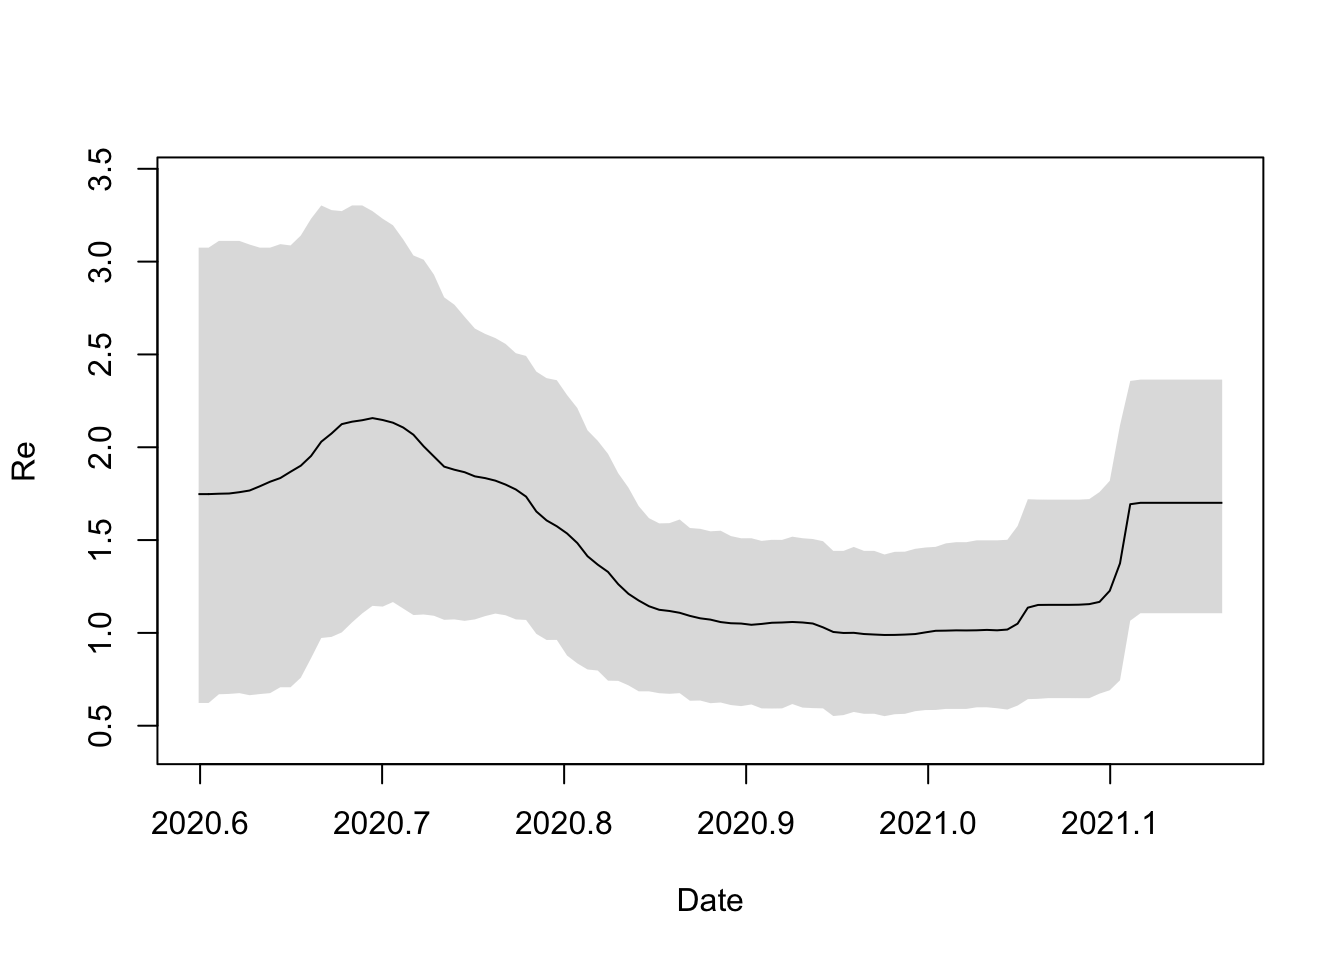
\includegraphics[width=0.60000\textwidth]{figures/plot-alpha-Re-1.png}
    \caption{The smooth $ R_e $ skyline.}
    \label{fig:bdsky_smooth}
\end{figure}

We can plot the gridded $R_e$ skyline (not its HPDs) for a
few of the MCMC samples to see what it really looks like as the Markov
chain samples parameters. Note that the intervals overlap between
different posterior samples. This is because the tMRCA is different in
each of the plotted samples. As we add more samples to the plot we start
to see the smooth skyline appear (Figure~\ref{fig:bdsky_traces}).

\begin{lstlisting}[language=R]
plotSkyline(times, Re_alpha_gridded, type='steplines', traces=1, 
            col=cols$blue,ylims=c(0,3.5), xlab="Time", ylab="R", main="1 random sample")
plotSkyline(times, Re_alpha_gridded, type='steplines', traces=10, 
                col=set_alpha(cols$blue,0.5),ylims=c(0,3.5), xlab="Time", ylab="R", main="10 random samples")
plotSkyline(times, Re_alpha_gridded, type='steplines', traces=100, 
                col=set_alpha(cols$blue,0.5),ylims=c(0,3.5), xlab="Time", ylab="R", main="100 random samples")
plotSkyline(times, Re_alpha_gridded, type='steplines', traces=1000, 
                col=set_alpha(cols$blue,0.1),ylims=c(0,3.5), xlab="Time", ylab="R", main="1000 random samples")
\end{lstlisting}

\begin{figure}
    \centering
    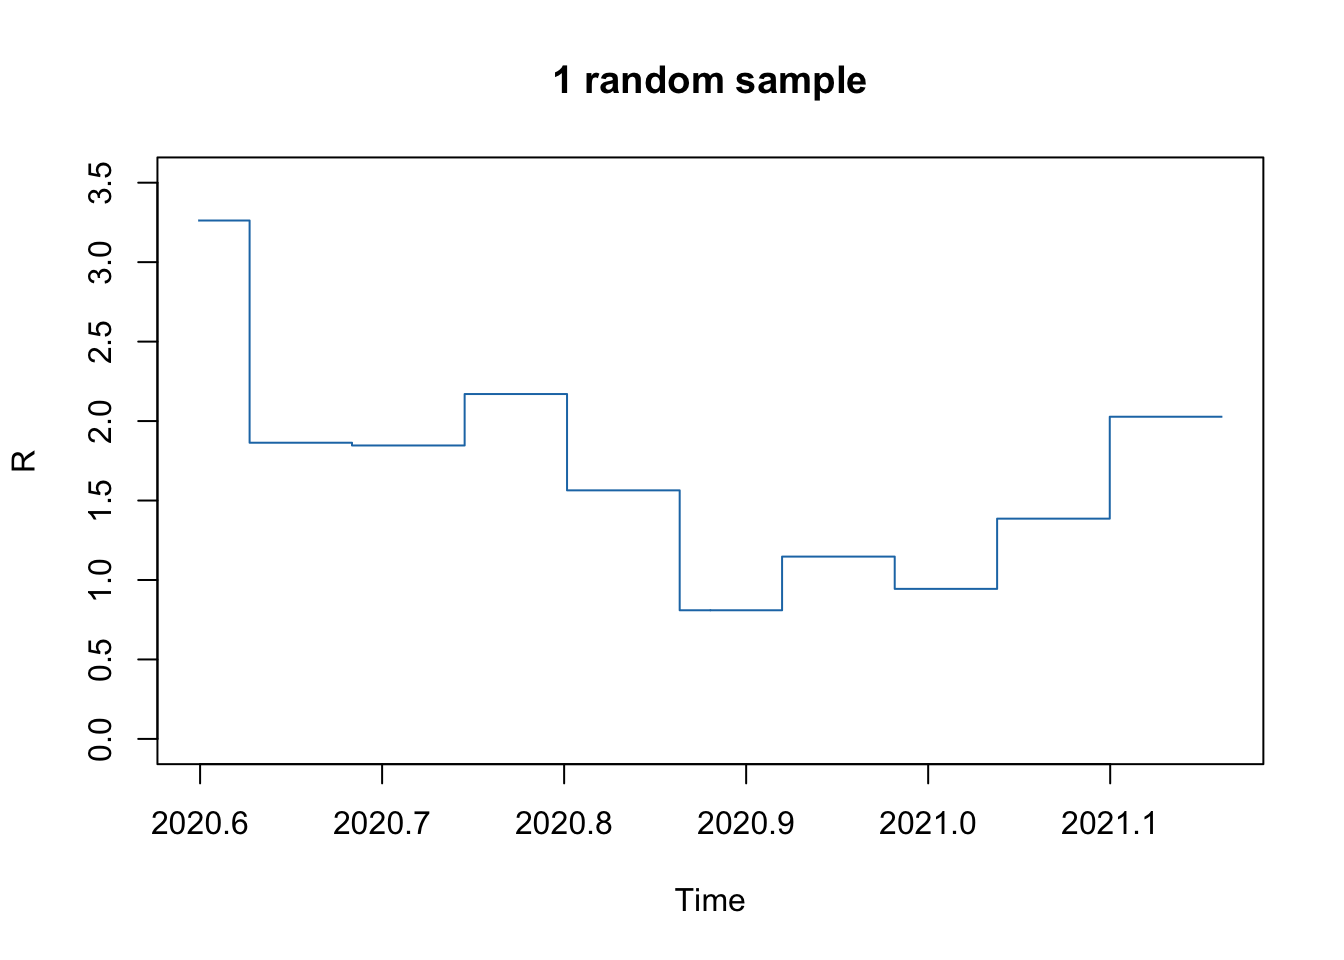
\includegraphics[width=0.450000\textwidth]{figures/plot-alpha-Re-traces-1.png}
    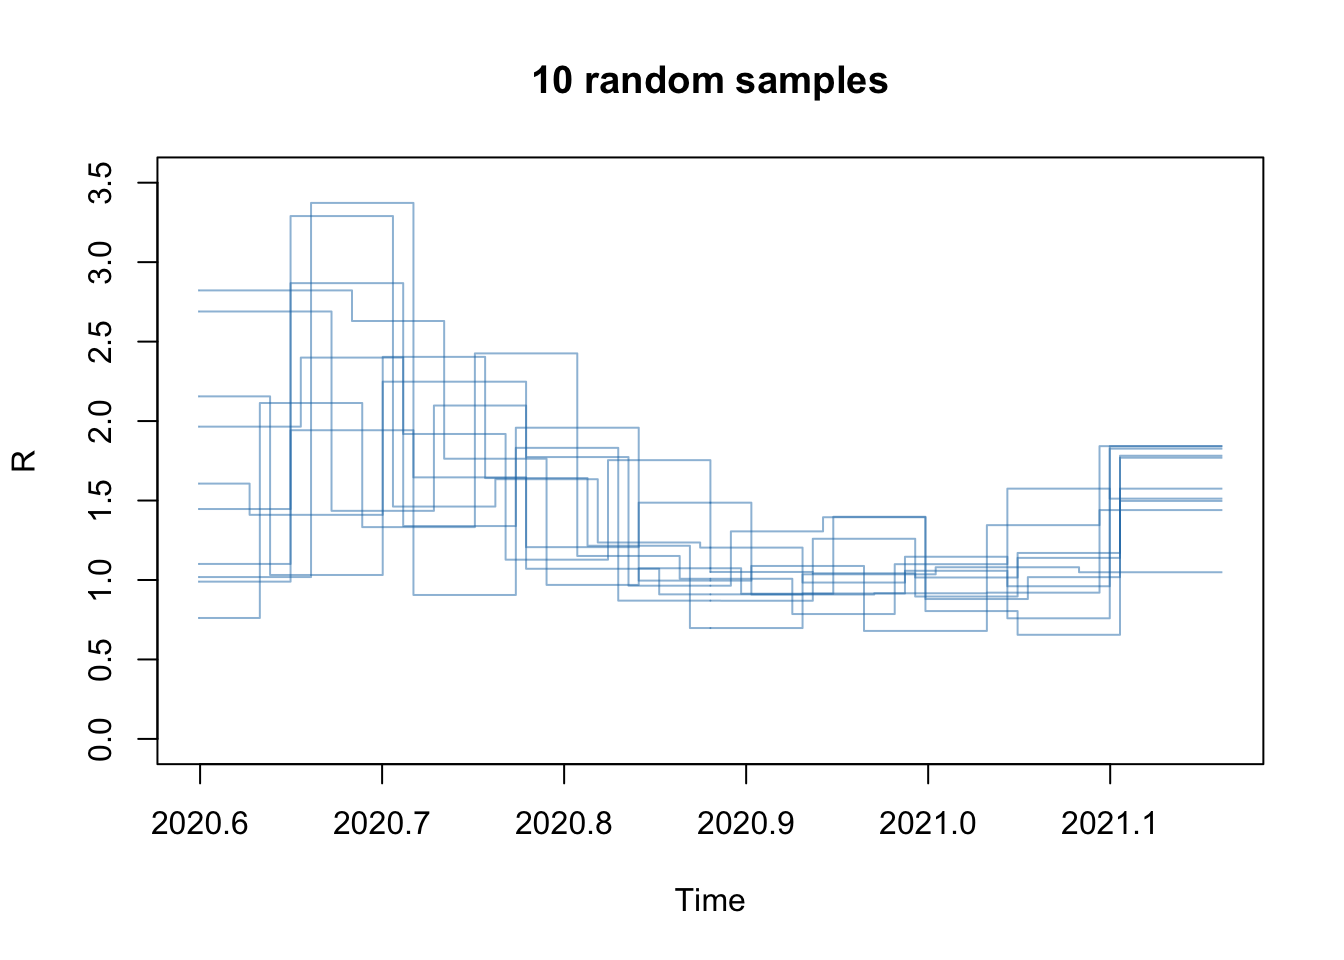
\includegraphics[width=0.450000\textwidth]{figures/plot-alpha-Re-traces-2.png}
    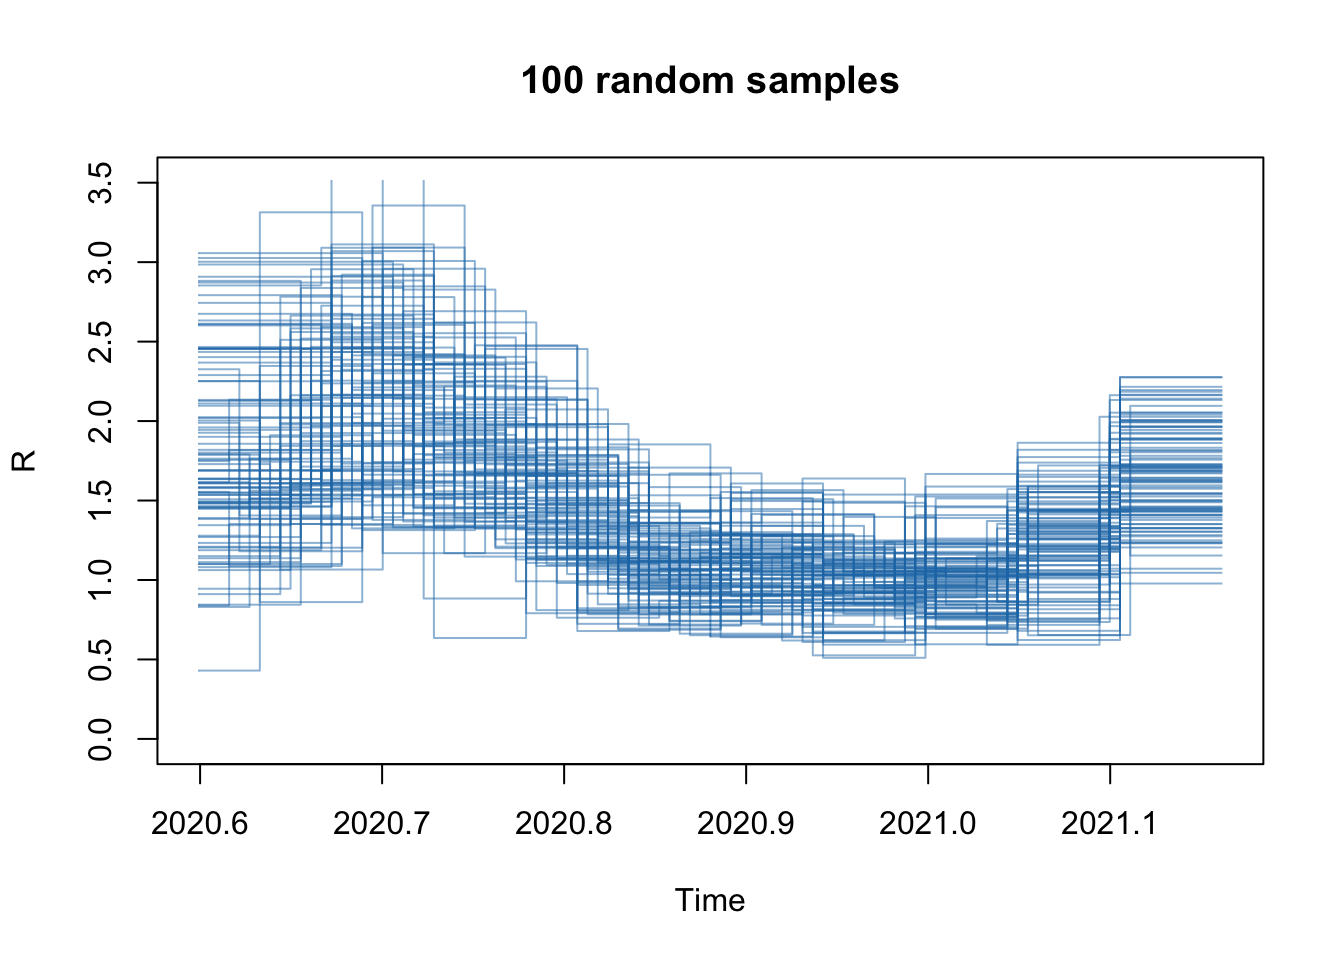
\includegraphics[width=0.450000\textwidth]{figures/plot-alpha-Re-traces-3.png}
    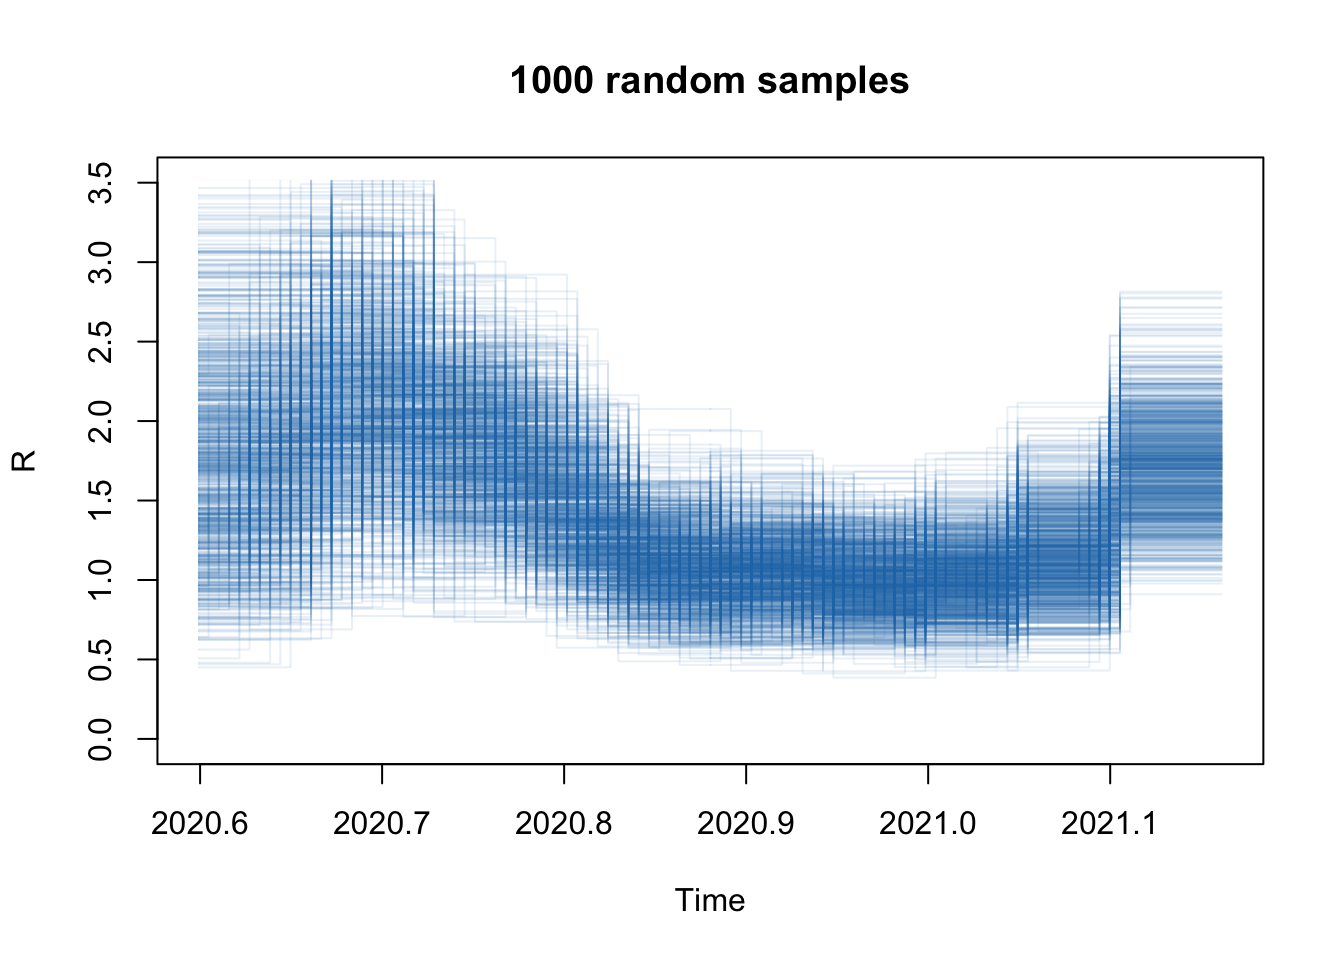
\includegraphics[width=0.450000\textwidth]{figures/plot-alpha-Re-traces-4.png}
    \caption{Increasing the number of traces plotted from 1 to 10, to 100, to 1000.}
    \label{fig:bdsky_traces}
\end{figure}


We can do the same for the sampling proportion estimates for the Alpha 
alignment (Figure~\ref{fig:bdsky_sampling}). 

\begin{figure}
    \centering
    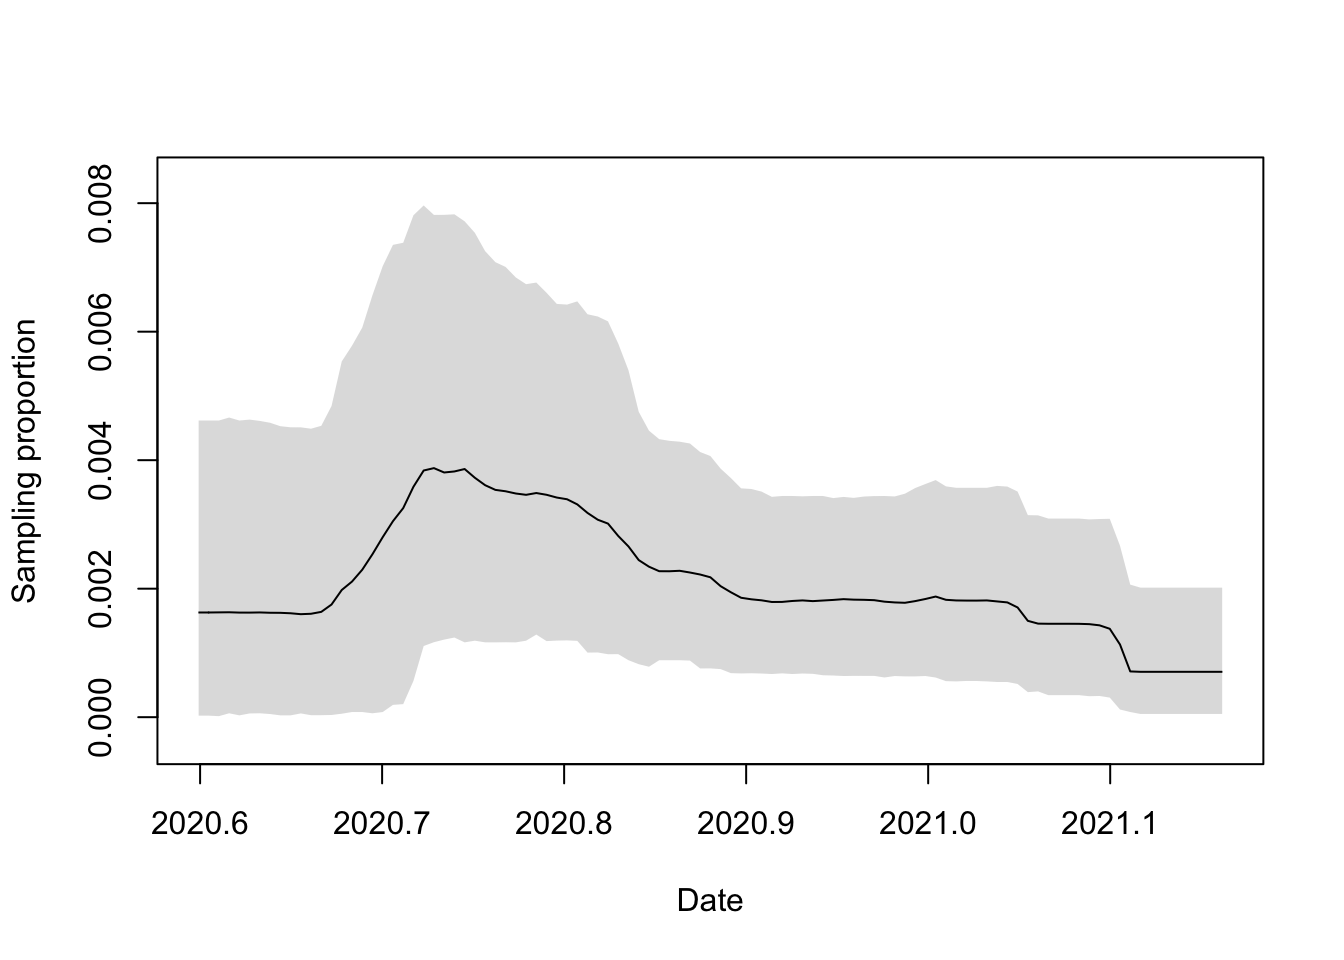
\includegraphics[width=0.600000\textwidth]{figures/alpha-samplingProp-1.png}
    \caption{The smooth sampling proportion skyline.}
    \label{fig:bdsky_sampling}
\end{figure}

\begin{lstlisting}[language=R]
samplingProp_alpha <- beastio::getLogFileSubset(bdsky_trace, "samplingProportion_BDSKY_SerialCondRoot.alpha")
samplingProp_alpha_gridded <- mcmc(bdskytools::gridSkyline(samplingProp_alpha, tmrca_alpha, gridTimes_alpha))
samplingProp_alpha_gridded_hpd <- t(getHPDMedian(samplingProp_alpha_gridded))
plotSkyline(lubridate::decimal_date(enddate)-gridTimes_alpha, samplingProp_alpha_gridded_hpd, 
            xlab="Date", ylab="Sampling proportion")   
\end{lstlisting}


Now we can follow the same steps to also extract and plot the skylines for the background alignment. 
Finally, we can plot both Alpha and the background datasets on one set of axes for comparison 
(Figure~\ref{fig:bdsky_combined}).

\begin{figure}
    \centering
    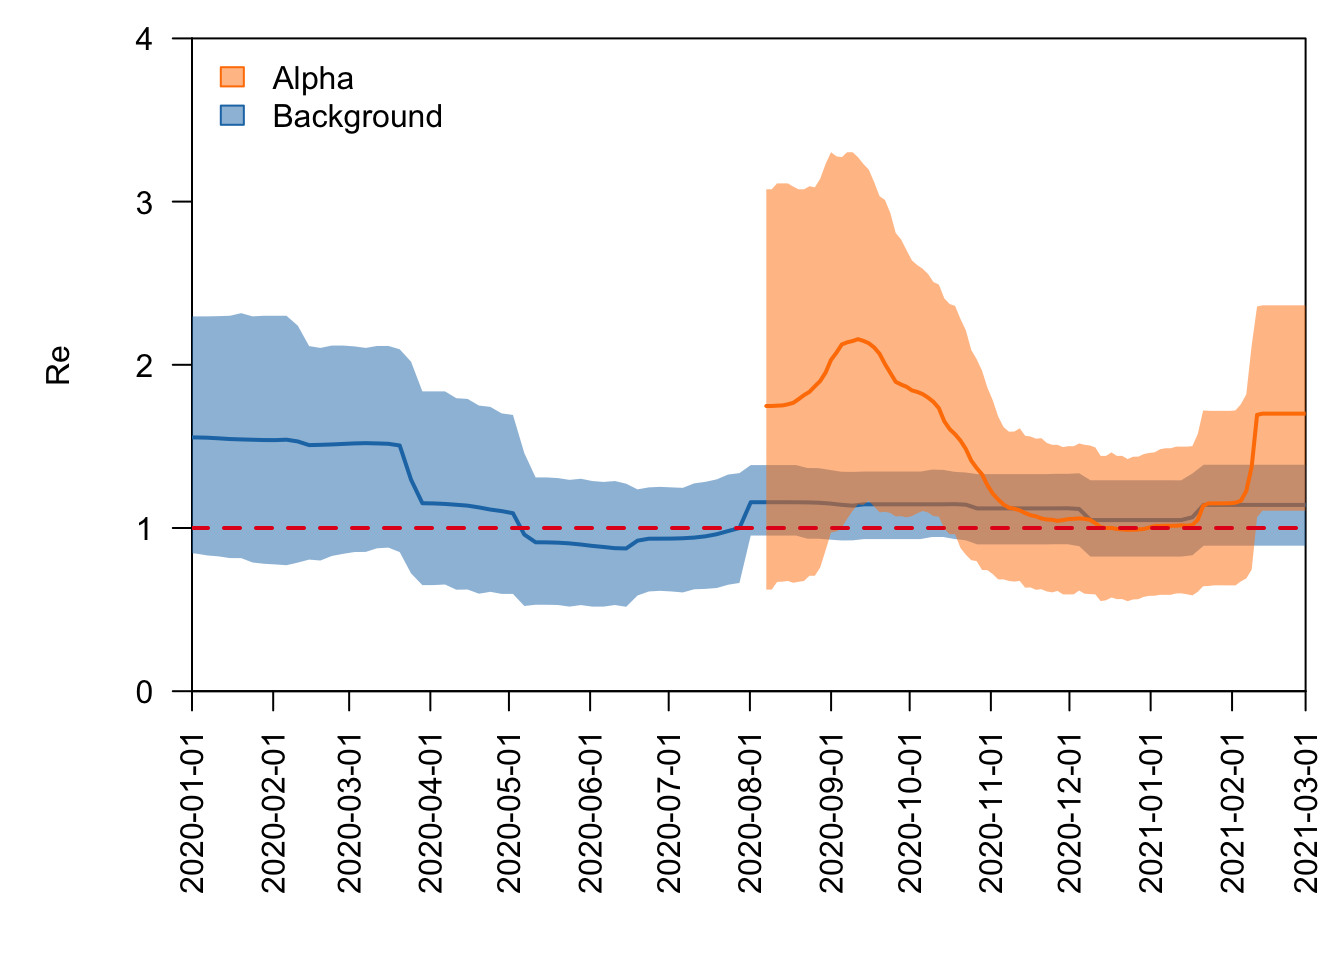
\includegraphics[width=0.600000\textwidth]{figures/combined-1.png}
    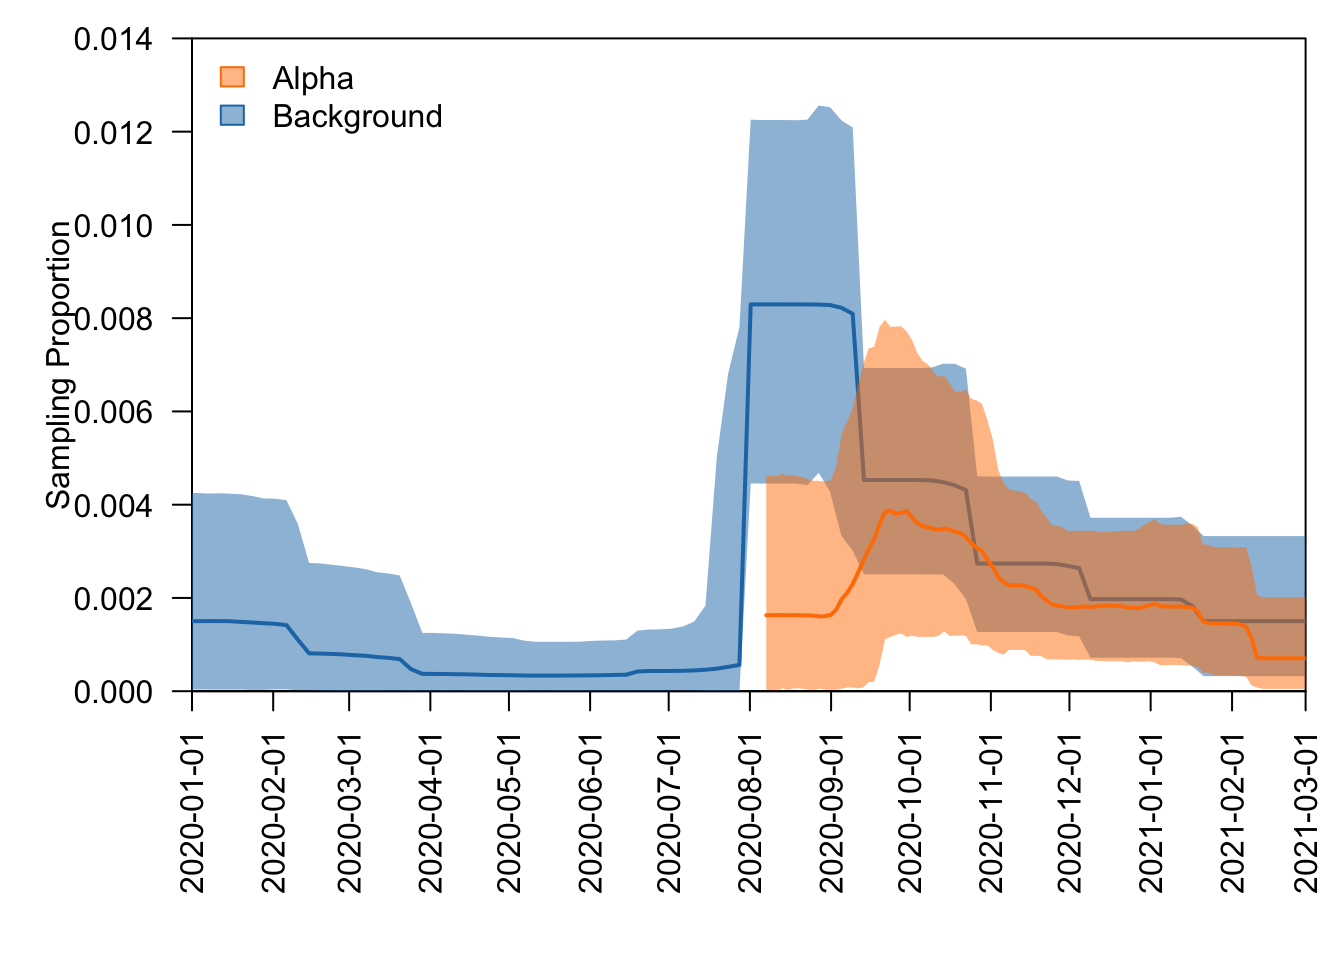
\includegraphics[width=0.600000\textwidth]{figures/combined-2.png}
    \caption{Plotting the skylines of the Alpha and background datasets on one set of axes.}
    \label{fig:bdsky_combined}
\end{figure}


\subsubsection{Comparing to the prior}

When comparing the posterior and prior estimates in Tracer we can see that for some parameters, 
such as the clock rates, the posterior is a much tighter and more peaked distribution than the prior
(Figure~\ref{fig:tracer_prior_post}). But for the Skyline parameters, the picture is much less clear. 
To get a better idea we have to plot the smooth skylines in R. 


\begin{figure}
    \centering
    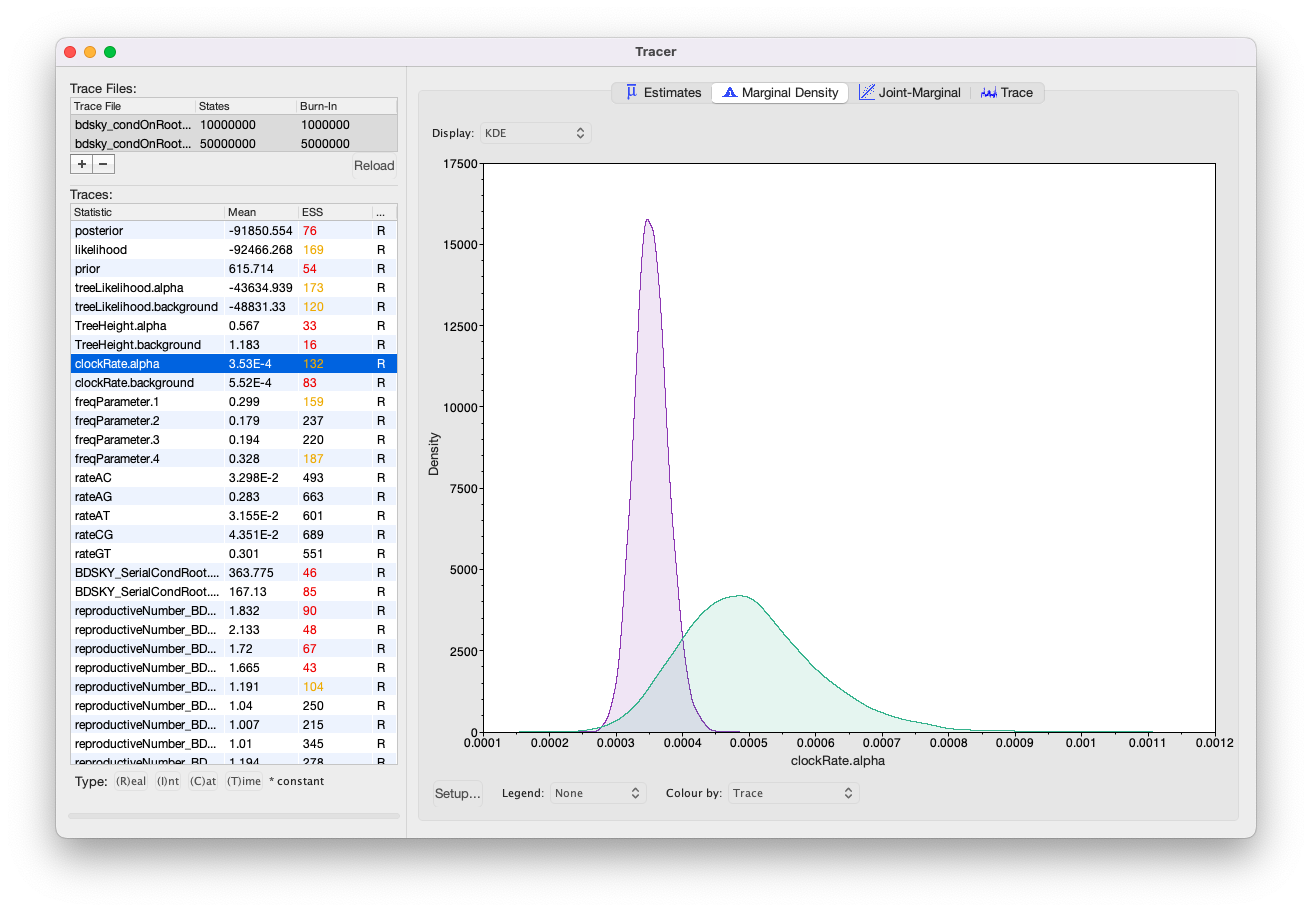
\includegraphics[max width=\textwidth, max height=0.9\textheight]{figures/tracer_prior_post.png}
    \caption{Comparing prior and posterior distributions in Tracer.}
    \label{fig:tracer_prior_post}
\end{figure}

We can follow the same steps as above to load the log file from 
\lstinline!bdsky_condOnRoot_samplingFromPrior_777.xml! into R, grid and plot the skylines, and then 
compare them to the posterior estimates (Figure~\ref{fig:bdsky_prior_post}).

\begin{figure}
    \centering
    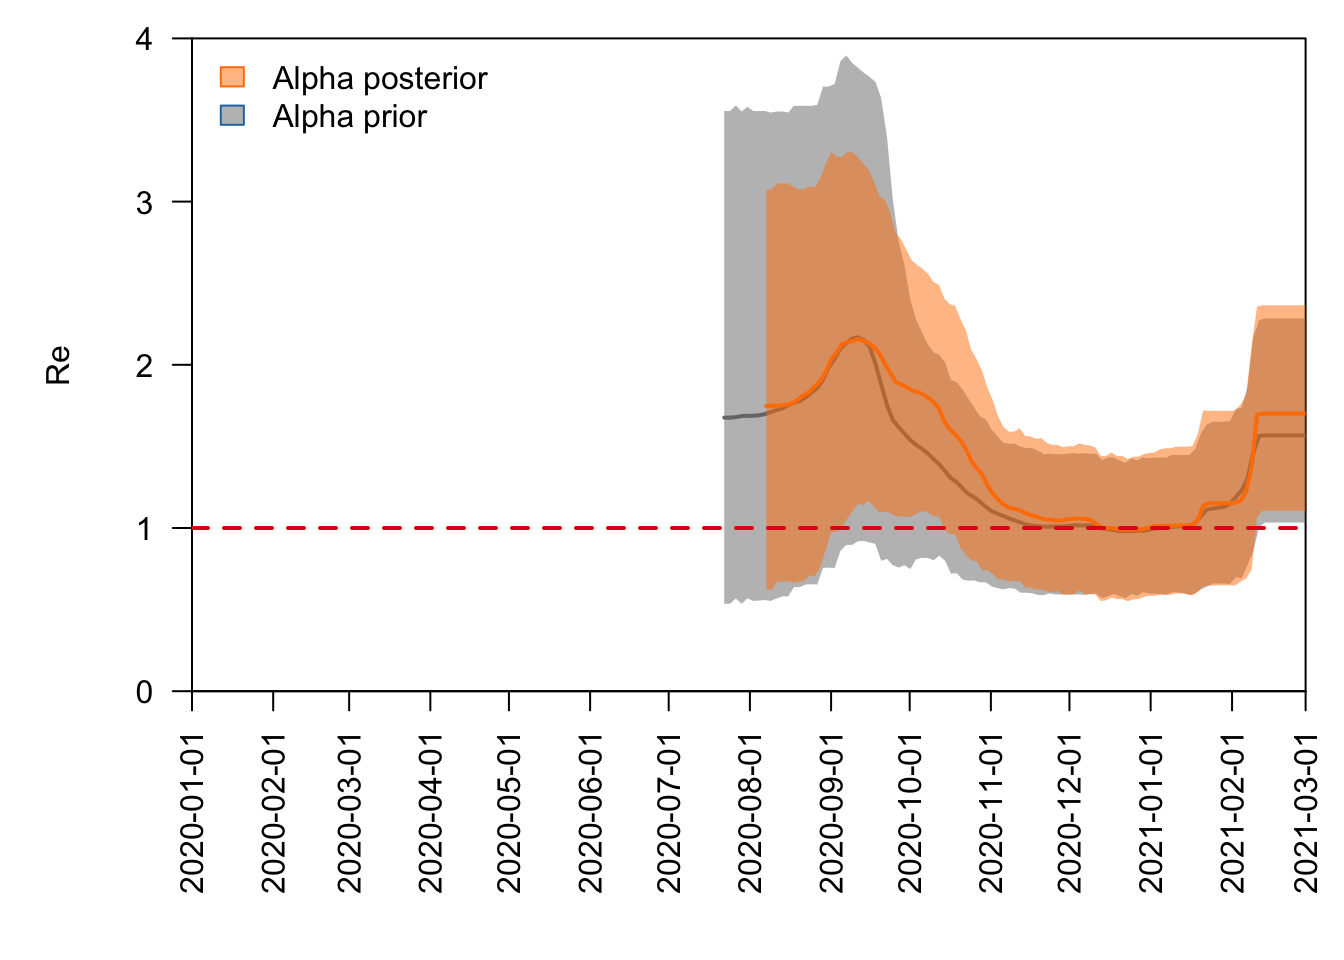
\includegraphics[max width=0.45\textwidth, max height=0.9\textheight]{figures/prior-comparison-1.png}
    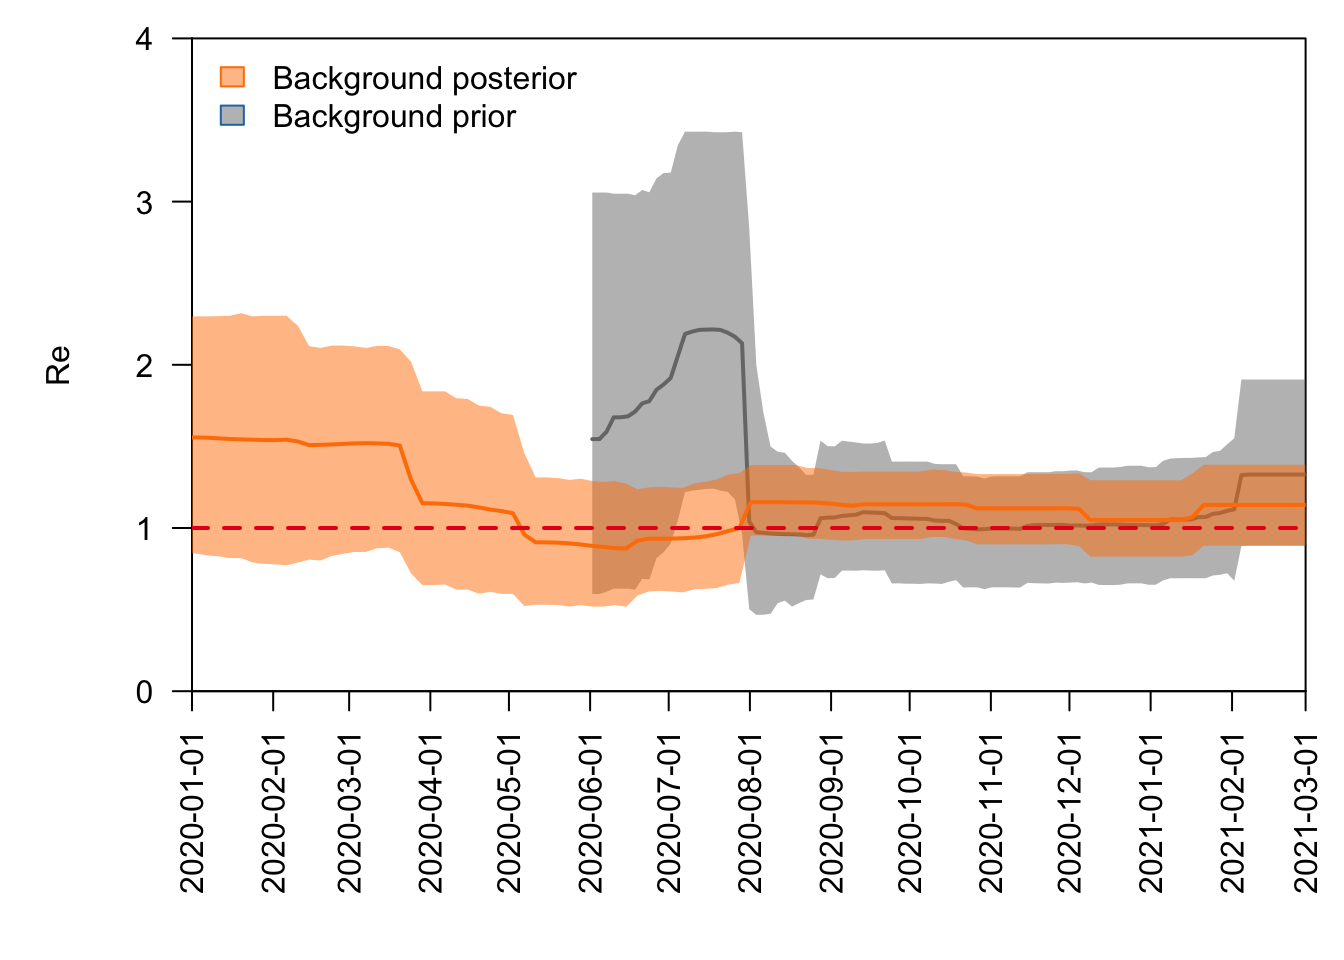
\includegraphics[max width=0.45\textwidth, max height=0.9\textheight]{figures/prior-comparison-2.png}
    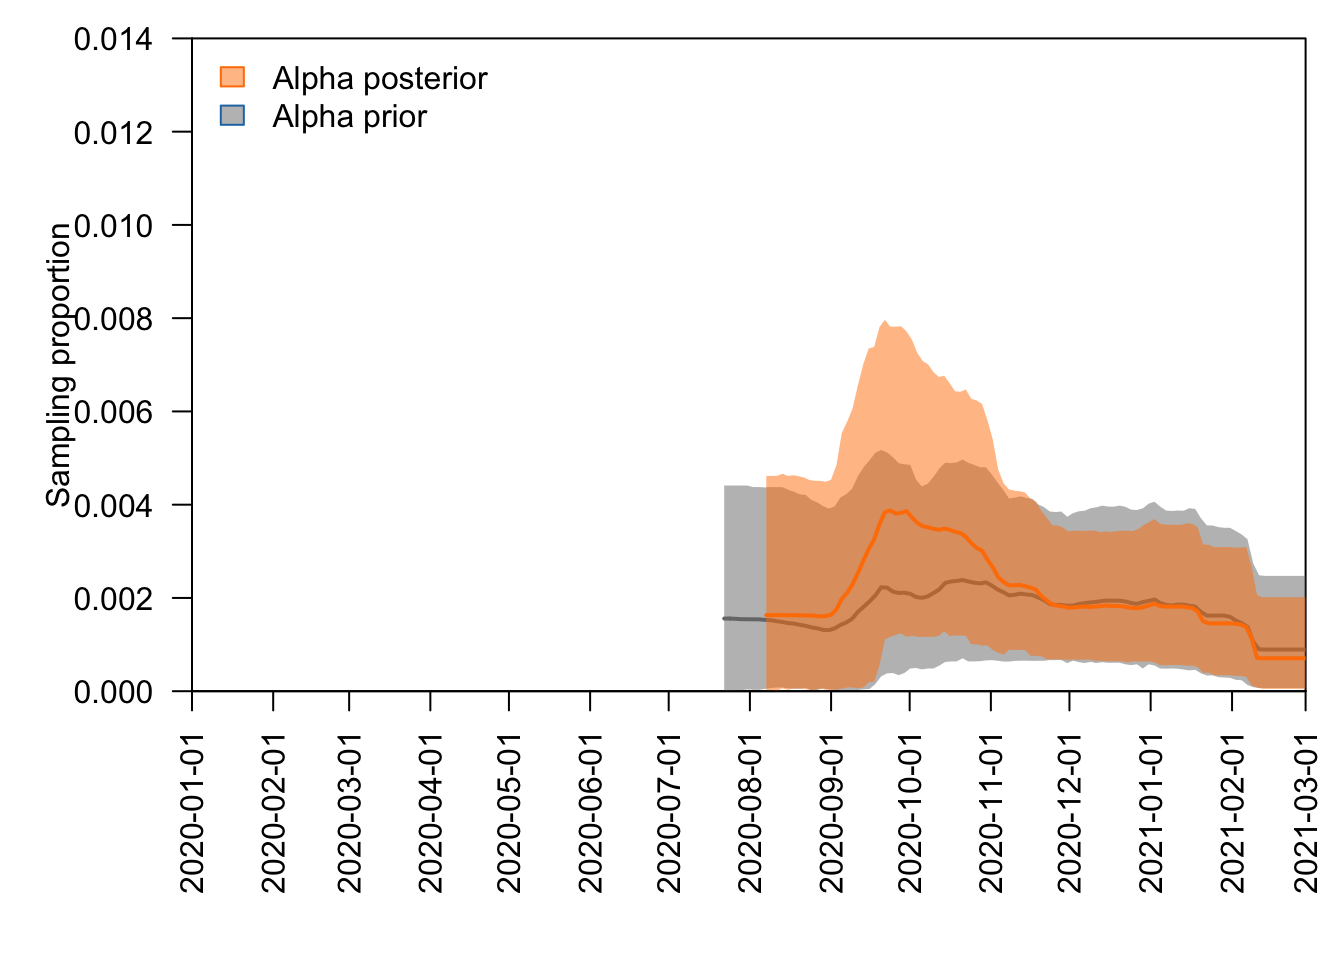
\includegraphics[max width=0.45\textwidth, max height=0.9\textheight]{figures/prior-comparison-3.png}
    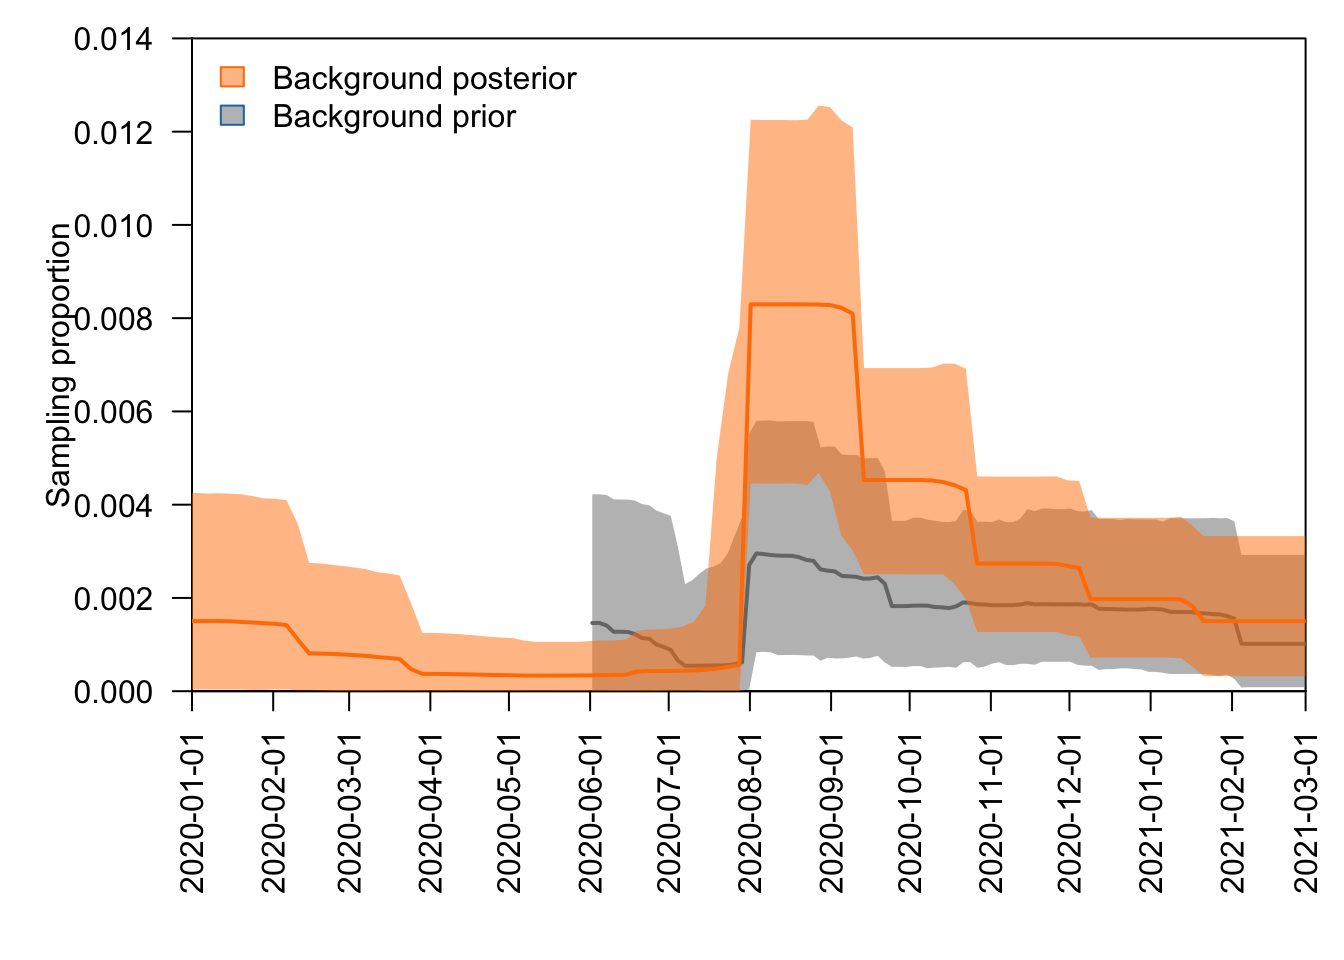
\includegraphics[max width=0.45\textwidth, max height=0.9\textheight]{figures/prior-comparison-4.png}
    \caption{Comparing prior and posterior distributions of the Birth Death Skyline parameters.}
    \label{fig:bdsky_prior_post}
\end{figure}


\clearpage

\subsection{Limitations}

Both the coalescent and the birth-death skylines assume that the
population is well-mixed. That is, they assume that there is no
significant population structure and that the sequences are a random
sample from the population. However, if there is population structure,
for instance sequences were sampled from two different villages and
there is much more contact within than between villages, then the
results will be biased \citep{Heller2013}. Instead a structured model
should then be used to account for these biases.

\begin{figure}
    \centering
    
\includegraphics[max width=\textwidth, max height=0.9\textheight]{figures/bsp_alpha_tree.png}
    \caption{The MCC tree of the Alpha alignment inferred by the Bayesian Skyline Plot.}
    \label{fig:bsp_alpha_tree}
\end{figure}

For the coalescent Bayesian Skyline plot we noticed that both skylines show a constant 
effective population size after November 2020 (Figure~\ref{fig:bsp_combined}). But 
this doesn't agree with what we know about the COVID-19 epidemic in the UK, where cases (especially of 
the Alpha VOC)
increased steeply over December 2020 and then started falling steeply after the New Year with 
the start of a lockdown. 

To understsand why the Bayesian Skyline Plot can't infer these dynamics on our dataset we have
to create the MCC trees in TreeAnnotator. We see that the MCC tree for the Alpha alignment has 
very long terminal branches, and many coalescent events deeper in the tree (Figure~\ref{fig:bsp_alpha_tree}).
This is indicative of fast exponential growth dynamics. When the population is large (in the present), 
the probability of two lineages coalescing is small, resulting in long terminal branches. When the 
population is small (in the past) the opposite is true, and brannch lengths are short, resulting in many
coalescent events. For the The Bayesian Skyline Plot only the coalescent events are informative of $N_e$. 
Therefore, the model detects fast growth during the period of many coalescent events (October/November 2020), 
but has no power to detect any changes in $N_e$ after this time. Because we only have a tiny sample of a 
huge epidemic wave, almost all of the coalescences in our tree occurred in October/November 2020. Had we 
taken a much larger sample it is possible that the model would have been able to infer more recent changes 
in $N_e$. In addition, there are variations of the coalescent model
that either assumes the growth rate remains constant (i.e. $N_e$ will keep growing) \citep{Volz2018} or 
so-called preferential sampling coalescent models that 
uses information from the sampling times to also inform $N_e$ \citep{Karcher2020, Parag2020, Karcher2016}. 

The Birth Death Skyline model uses both coalescent and sampling events to inform itself about the rates.
However, it is apparent that our datasets are not informative enough to allow for tight estimates of 
$R_e$ (Figure~\ref{fig:bdsky_combined}). It is also apparent that most of the information for the Alpha
$R_e$ and sampling proportion estimates come from the sampling times, 
and not the sequences (Figure~\ref{fig:bdsky_prior_post}). 
This is also true to some extent for the background alignment, although the posterior estimates deviate 
more from the prior. 

With the background sampling proportion it is interesting to note that the estimates
include 0 in their HPDs until August 1st, 2020, the time of the oldest sample in our dataset. After that, 
the sampling proportion jumps and then decreases again. This agrees with the situation in the UK at the 
time, where cases were very low during August, but started increasing from September 2020. 
Usually, we would want to set the sampling proportion to 0 before our oldest sample. At the moment this 
requires editing the XML file. See \href{https://github.com/laduplessis/skylinetools/wiki/TreeSlicer}{here}
for more information on how to do this or \textbf{ask me for help}! 

Because SARS-CoV-2 evolves relatively slowly (around 2 \emph{de novo} mutations per month) sequences are 
not that informative over short time scales. That means larger datasets or extra information need to be 
included in order to make accurate inferences. 


\clearpage




%%%%%%%%%%%%%%%%%%%%%%%
% Tutorial disclaimer %
%%%%%%%%%%%%%%%%%%%%%%%
% Please do not change the license
% Add the author names and relevant links
% Add any other aknowledgments here
\href{http://creativecommons.org/licenses/by/4.0/}{
\includegraphics[scale=0.8]{figures/ccby.pdf}} This tutorial was written by Louis du Plessis and is licensed under a \href{http://creativecommons.org/licenses/by/4.0/}{Creative Commons Attribution 4.0 International License}. 


%%%%%%%%%%%%%%%%%%%%
% Do NOT edit this %
%%%%%%%%%%%%%%%%%%%%
Version dated: \today


%%%%%%%%%%%%%%%%
%  REFERENCES  %
%%%%%%%%%%%%%%%%

\printbibliography


\end{document}